% =====================================================================
% TCC 1 - Engenharia de Software - UnB/FCTE
% Template: abnTeX2
% Compilar: pdflatex main && bibtex main && pdflatex main && pdflatex main
% Nota sobre Figuras: se os arquivos PNG estiverem em ./figuras/, eles
% sao carregados automaticamente; caso contrario, o documento renderiza
% diagramas vetoriais nativos em TikZ (zero placeholders "[Inserir...]").
% =====================================================================
\documentclass[12pt,openany,oneside,a4paper,english,brazilian,sumario=tradicional]{abntex2}

\usepackage{lmodern}
\usepackage[T1]{fontenc}
\usepackage[utf8]{inputenc}
\usepackage{indentfirst}
\usepackage{xcolor}
\usepackage{graphicx}
\usepackage{amsmath,amssymb}
\usepackage{booktabs}
\usepackage{tabularx}
\usepackage{array}
\usepackage{enumitem}
% Carrega TikZ apenas se alguma das 8 figuras PNG nao estiver presente em ./figuras/
\newif\ifallfigspresent
\allfigspresenttrue
\IfFileExists{figuras/fig01_dag_exemplo.png}{}{\allfigspresentfalse}
\IfFileExists{figuras/fig02_pert_beta.png}{}{\allfigspresentfalse}
\IfFileExists{figuras/fig03_niveis_gemeo_digital.png}{}{\allfigspresentfalse}
\IfFileExists{figuras/fig04_hash_chain.png}{}{\allfigspresentfalse}
\IfFileExists{figuras/fig05_arquitetura.png}{}{\allfigspresentfalse}
\IfFileExists{figuras/fig06_sequencia.png}{}{\allfigspresentfalse}
\IfFileExists{figuras/fig07_histograma_cdf_poc.png}{}{\allfigspresentfalse}
\IfFileExists{figuras/fig08_gantt.png}{}{\allfigspresentfalse}
\ifallfigspresent\else
  \usepackage{tikz}%
  \usetikzlibrary{arrows.meta,positioning,shapes.geometric,calc}%
\fi
\IfFileExists{resultados_poc.tex}{% Arquivo gerado automaticamente por Codigo/main.go (N = 10.000, seed = 42)
% Nao edite manualmente; execute "cd Codigo && go run ." para atualizar.
\providecommand{\pocACPM}{10.83}
\providecommand{\pocAPcinquenta}{11.39}
\providecommand{\pocAPoitentaeCinco}{12.75}
\providecommand{\pocAPnoventaeCinco}{13.64}
\providecommand{\pocAProbMeta}{38.3}
\providecommand{\pocBCPM}{10.83}
\providecommand{\pocBPcinquenta}{11.79}
\providecommand{\pocBPoitentaeCinco}{13.43}
\providecommand{\pocBPnoventaeCinco}{14.55}
\providecommand{\pocBProbMeta}{29.4}
\providecommand{\pocCCPM}{11.02}
\providecommand{\pocCPcinquenta}{11.47}
\providecommand{\pocCPoitentaeCinco}{12.77}
\providecommand{\pocCPnoventaeCinco}{13.55}
\providecommand{\pocCProbMeta}{32.2}
\providecommand{\pocCPrimeCPM}{11.02}
\providecommand{\pocCPrimePcinquenta}{11.14}
\providecommand{\pocCPrimePoitentaeCinco}{12.20}
\providecommand{\pocCPrimePnoventaeCinco}{12.89}
\providecommand{\pocCPrimeProbMeta}{43.3}
\providecommand{\tccDoisBaseCPM}{16.75}
\providecommand{\tccDoisBasePcinquenta}{16.80}
\providecommand{\tccDoisBasePoitentaeCinco}{17.51}
\providecommand{\tccDoisBasePnoventaeCinco}{17.94}
\providecommand{\tccDoisBaseProbVinte}{100.0}
\providecommand{\tccDoisRiscosPcinquenta}{17.29}
\providecommand{\tccDoisRiscosPoitentaeCinco}{18.30}
\providecommand{\tccDoisRiscosPnoventaeCinco}{18.92}
\providecommand{\tccDoisRiscosProbVinte}{99.6}
}{}
\usepackage[brazilian,hyperpageref]{backref}
\usepackage[alf]{abntex2cite}
\usepackage{eso-pic}
\usepackage{hyperref}

\newcolumntype{L}[1]{>{\raggedright\arraybackslash}p{#1}}
\newcolumntype{Y}{>{\raggedright\arraybackslash}X}

\definecolor{unbblue}{HTML}{1D4B7C}
\definecolor{unbgreen}{HTML}{008C4F}
\hypersetup{colorlinks=true,linkcolor=unbblue,citecolor=unbblue,urlcolor=unbblue}

\renewcommand{\backrefpagesname}{Citado na(s) página(s):}
\renewcommand*{\backref}[1]{}
\renewcommand*{\backrefalt}[4]{%
  \ifcase #1 Nenhuma citação no texto.%
  \or Citado na página #2.%
  \else Citado #1 vezes nas páginas #2.\fi}

% Macro de figura com fallback vetorial em TikZ (elimina placeholders vazios)
\newcommand{\figura}[5]{%
  \begin{figure}[htbp]
    \caption{#2}\label{#3}
    \centering
    \IfFileExists{figuras/#1}%
      {\includegraphics[width=#4\textwidth]{figuras/#1}}%
      {#5}%
    \par\vspace{2mm}\small Fonte: Elaborado pelos autores (2026).
  \end{figure}%
}

\newcommand{\figuraAdaptada}[6]{%
  \begin{figure}[htbp]
    \caption{#2}\label{#3}
    \centering
    \IfFileExists{figuras/#1}%
      {\includegraphics[width=#4\textwidth]{figuras/#1}}%
      {#5}%
    \par\vspace{2mm}\small Fonte: Adaptado de #6 pelos autores (2026).
  \end{figure}%
}

\newcommand{\fonteautores}{\par\vspace{1mm}{\small Fonte: Elaborado pelos autores (2026).}}
\newcommand{\IC}{\mathrm{IC}}

% Reduz espacos em branco causados por flutuantes (figuras e tabelas)
\renewcommand{\topfraction}{0.9}
\renewcommand{\bottomfraction}{0.9}
\renewcommand{\textfraction}{0.1}
\renewcommand{\floatpagefraction}{0.8}

\titulo{Sombra Digital Governada e Inteligência Artificial para Apoio à Decisão em Projetos de Software: Arquitetura de Referência com Simulação de Monte Carlo e Governança Humana}
\autor{Carlos Henrique de Souza Bispo, Paulo Henrique Virgilio Cerqueira}
\local{Brasília, DF}
\data{2026}
\orientador{Prof. Dr. Ricardo Matos Chaim}
\instituicao{Universidade de Brasília - UnB\par Faculdade de Ciências e Tecnologias em Engenharia - FCTE}
\tipotrabalho{Trabalho de Conclusão de Curso}
\preambulo{Monografia submetida ao curso de graduação em Engenharia de Software da Universidade de Brasília, como requisito parcial para obtenção do Título de Bacharel em Engenharia de Software.}

\setlength{\parindent}{1.3cm}
\setlength{\parskip}{0.2cm}

\begin{document}
\selectlanguage{brazilian}
\shorthandoff{"}
\frenchspacing

% ------------------------------------------------------------ CAPA
\begin{capa}
  \IfFileExists{capa_fundo.jpg}{%
    \AddToShipoutPictureBG*{\AtPageLowerLeft{\includegraphics[width=\paperwidth,height=\paperheight]{capa_fundo.jpg}}}%
  }{%
    \IfFileExists{capa_fundo.png}{%
      \AddToShipoutPictureBG*{\AtPageLowerLeft{
\includegraphics[width=\paperwidth,height=\paperheight]{capa_fundo.png}}}%
    }{}%
  }
  \centering
  \vspace*{7.2cm}
  {\color{unbblue}\bfseries Universidade de Brasília \textendash{} UnB\par
  Faculdade de Ciências e Tecnologias em Engenharia \textendash{} FCTE\par
  Engenharia de \textit{Software}\par}
  \vspace*{1.6cm}
  {\sffamily\bfseries\large Sombra Digital Governada e Inteligência Artificial para Apoio à Decisão em Projetos de Software: Arquitetura de Referência com Simulação de Monte Carlo e Governança Humana\par}
  \vspace*{1.4cm}
  {\bfseries Autores: Carlos Henrique de Souza Bispo, Paulo Henrique Virgilio Cerqueira\par
  \vspace{0.4cm}
  Orientador: Prof. Dr. Ricardo Matos Chaim\par}
  \vspace{0.8cm}
  Brasília, DF\par 2026
\end{capa}

% ------------------------------------------------------------ FOLHA DE ROSTO
\begin{center}
  {\bfseries Carlos Henrique de Souza Bispo, Paulo Henrique Virgilio Cerqueira}\par
  \vspace{3cm}
  {\bfseries\large Sombra Digital Governada e Inteligência Artificial para Apoio à Decisão em Projetos de Software: Arquitetura de Referência com Simulação de Monte Carlo e Governança Humana}\par
  \vspace{2cm}
  \begin{flushright}
  \begin{minipage}{0.55\textwidth}
  \small Monografia submetida ao curso de graduação em Engenharia de Software da Universidade de Brasília, como requisito parcial para obtenção do Título de Bacharel em Engenharia de Software.
  \end{minipage}
  \end{flushright}
  \vspace{2cm}
  Universidade de Brasília - UnB\par
  Faculdade de Ciências e Tecnologias em Engenharia - FCTE\par
  \vspace{0.5cm}
  Orientador: Prof. Dr. Ricardo Matos Chaim\par
  \vfill
  Brasília, DF\par 2026
\end{center}
\clearpage

% ------------------------------------------------------------ FOLHA DE APROVAÇÃO
\begin{center}
  {\bfseries Carlos Henrique de Souza Bispo, Paulo Henrique Virgilio Cerqueira}\par
  \vspace{1cm}
  {\bfseries Sombra Digital Governada e Inteligência Artificial para Apoio à Decisão em Projetos de Software: Arquitetura de Referência com Simulação de Monte Carlo e Governança Humana}\par
  \vspace{1cm}
  \begin{flushright}
  \begin{minipage}{0.55\textwidth}
  \small Monografia submetida ao curso de graduação em Engenharia de Software da Universidade de Brasília, como requisito parcial para obtenção do Título de Bacharel em Engenharia de Software.
  \end{minipage}
  \end{flushright}
  \vspace{1cm}
  Trabalho aprovado. Brasília, DF, \rule{1.2cm}{0.4pt} de \rule{3.8cm}{0.4pt} de 2026:\par
  \vspace{1.8cm}
  \rule{9cm}{0.4pt}\par Prof. Dr. Ricardo Matos Chaim\par Orientador (UnB/FCTE)\par
  \vspace{1.2cm}
  \rule{9cm}{0.4pt}\par Membro Examinador Interno (UnB/FCTE)\par
  \vspace{1.2cm}
  \rule{9cm}{0.4pt}\par Membro Examinador Interno (UnB/FCTE)\par
  \vfill
  Brasília, DF\par 2026
\end{center}
\clearpage

% ------------------------------------------------------------ RESUMO
\begin{resumo}
Projetos de software em ciclos iterativos ou híbridos enfrentam incerteza de prazos causada por dependências técnicas entre componentes, estimativas humanas sujeitas a vieses cognitivos e impedimentos operacionais. As ferramentas atuais registram tarefas de forma passiva, e a ausência de ligação entre eventos de engenharia e modelos formais de rede dificulta a detecção precoce de desvios no caminho crítico. Ao mesmo tempo, o uso não governado de Modelos de Linguagem de Larga Escala (LLMs) em sistemas corporativos expõe vulnerabilidades como injeção indireta de comandos, divulgação de informações sensíveis, tratamento inseguro de saída, agência excessiva e consumo ilimitado, além de divergências numéricas em sínteses estocásticas. Este trabalho especifica a arquitetura proposta de um sistema de apoio à decisão concebido, segundo a taxonomia de Kritzinger, como uma Sombra Digital de processo com atuação governada sobre o modelo virtual, constituindo um degrau arquitetural controlado rumo a Gêmeos Digitais de processo. A solução articula captura automatizada de eventos de repositórios e integração contínua (GitHub/CI), cálculo determinístico do caminho crítico (CPM), Simulação de Monte Carlo (distribuição PERT-Beta acoplada a riscos discretos de Bernoulli) e recomendações interpretativas geradas por um LLM isolado que recebe apenas metadados sanitizados (\textit{allowlist}). A governança baseia-se em classificação binária de impacto no servidor com negação por padrão (\textit{fail-closed}), retenção de ações críticas para aprovação humana com exibição segregada do impacto simulado e trilha de auditoria encadeada por SHA-256 resistente a adulterações (\textit{tamper-evident}) com ancoragem externa. A viabilidade do motor estocástico foi verificada por uma Prova de Conceito (PoC) reprodutível em Go: o amostrador PERT-Beta foi verificado analiticamente e por teste de Kolmogorov-Smirnov (incluindo o caso degenerado $t_o=t_p$), o CPM contra o cálculo manual, a execução com 1, 4 e 16 \textit{workers} produziu resultados idênticos em quantis e média compensada de Kahan, e 10.000 iterações levaram mediana de 5,8 ms em uma rede de 4 tarefas (1 \textit{worker}) e 62,3 ms (8 \textit{workers}; 259,6 ms em 1 núcleo) em uma rede sintética de 200 tarefas e 300 dependências. O trabalho também caracteriza janelas de \textit{release} do repositório GitHub CLI (\texttt{cli/cli}) para \textit{backtesting}, contrastando o tempo de revisão do PR com a duração de engenharia desde o primeiro \textit{commit}, e apresenta o cronograma pré-registrado do TCC2 em 20 semanas para dois autores, cuja simulação de Monte Carlo indica $P_{50}=17{,}29$ e $P_{85}=18{,}30$ semanas ($P(F \le 20)=99{,}6\%$ com riscos discretos).

\textbf{Palavras-chave}: Sombra Digital de Processo, Gêmeo Digital, Simulação de Monte Carlo, Método do Caminho Crítico, Governança de Inteligência Artificial, Engenharia de Software.
\end{resumo}

\begin{resumo}[Abstract]
\begin{otherlanguage*}{english}
Software projects in iterative or hybrid lifecycles face schedule uncertainty caused by technical dependencies, human estimation biases, and operational impediments. Contemporary tools record work items passively, and the lack of coupling between engineering events and formal network models hinders early detection of critical path shifts. Meanwhile, ungoverned adoption of Large Language Models (LLMs) in enterprise systems exposes vulnerabilities such as indirect prompt injection, sensitive information disclosure, improper output handling, excessive agency, and unbounded consumption, besides numerical divergences in stochastic summaries. This work specifies the proposed architecture of a decision-support system designed, under Kritzinger's taxonomy, as a process Digital Shadow with governed in-model actuation, serving as a controlled architectural stepping stone toward process Digital Twins. The architecture integrates automated event capture from version control and continuous integration (GitHub/CI), deterministic Critical Path Method (CPM), Monte Carlo Simulation (PERT-Beta distribution coupled with Bernoulli discrete risks), and explanatory recommendations produced by an isolated LLM agent restricted to a sanitized metadata allowlist. Governance relies on server-side binary impact classification with default denial (\textit{fail-closed}), human approval of restricted actions with segregated simulated impact preview, and tamper-evident SHA-256 hash-chained audit logging with external anchoring. Algorithmic feasibility was verified through a reproducible Go Proof of Concept (PoC): the PERT-Beta sampler was verified analytically and via Kolmogorov-Smirnov goodness-of-fit testing (including the degenerate case $t_o=t_p$), the CPM matched hand calculation, runs with 1, 4, and 16 workers produced identical quantiles and Kahan-compensated means, and 10,000 iterations took a median of 5.8 ms on a 4-task network (1 worker) and 62.3 ms (8 workers; 259.6 ms on 1 core) on a synthetic 200-task/300-dependency network. The work also characterizes GitHub CLI (\texttt{cli/cli}) release windows for backtesting, contrasting PR review time against engineering duration from the first commit, and presents the pre-registered 20-week TCC2 schedule for two authors, whose Monte Carlo simulation yields $P_{50}=17.29$ and $P_{85}=18.30$ weeks ($P(F \le 20)=99.6\%$ with discrete risks).

\textbf{Keywords}: Process Digital Shadow, Digital Twin, Monte Carlo Simulation, Critical Path Method, AI Governance, Software Engineering.
\end{otherlanguage*}
\end{resumo}

% ------------------------------------------------------------ LISTAS
\pdfbookmark[0]{\listfigurename}{lof}
\listoffigures*
\cleardoublepage
\pdfbookmark[0]{\listtablename}{lot}
\listoftables*
\cleardoublepage

\begin{siglas}
  \item[ACID] Atomicidade, Consistência, Isolamento e Durabilidade
  \item[API] \textit{Application Programming Interface}
  \item[CA] Critério de Aceitação
  \item[CDF] \textit{Cumulative Distribution Function} (Função de Distribuição Acumulada)
  \item[CI/CD] \textit{Continuous Integration / Continuous Delivery}
  \item[CPM] \textit{Critical Path Method} (Método do Caminho Crítico)
  \item[CRN] \textit{Common Random Numbers} (Números Aleatórios Comuns)
  \item[CRPS] \textit{Continuous Ranked Probability Score}
  \item[CRUD] \textit{Create, Read, Update, Delete}
  \item[DAG] \textit{Directed Acyclic Graph} (Grafo Acíclico Dirigido)
  \item[DSRM] \textit{Design Science Research Methodology}
  \item[FS] \textit{Finish-to-Start} (Término-a-Início)
  \item[HMAC] \textit{Hash-based Message Authentication Code}
  \item[HSM] \textit{Half-Sample Mode} (Estimador de Moda por Meia-Amostra)
  \item[IC] Índice de Criticidade
  \item[JWT] \textit{JSON Web Token}
  \item[KS] Kolmogorov-Smirnov
  \item[LLM] \textit{Large Language Model} (Modelo de Linguagem de Larga Escala)
  \item[MAE] \textit{Mean Absolute Error} (Erro Médio Absoluto)
  \item[MCSE] \textit{Monte Carlo Standard Error} (Erro-Padrão de Monte Carlo)
  \item[MVP] \textit{Minimum Viable Product}
  \item[NMAE] \textit{Normalized Mean Absolute Error} (Erro Médio Absoluto Normalizado)
  \item[OFAT] \textit{One-Factor-at-a-Time} (Sensibilidade Um-Fator-por-Vez)
  \item[OWASP] \textit{Open Web Application Security Project}
  \item[PERT] \textit{Program Evaluation and Review Technique}
  \item[PII] \textit{Personally Identifiable Information}
  \item[PMBOK] \textit{Project Management Body of Knowledge}
  \item[PMI] \textit{Project Management Institute}
  \item[PoC] \textit{Proof of Concept} (Prova de Conceito)
  \item[PR] \textit{Pull Request}
  \item[PRNG] \textit{Pseudo-Random Number Generator}
  \item[RBAC] \textit{Role-Based Access Control}
  \item[RCPSP] \textit{Resource-Constrained Project Scheduling Problem}
  \item[RF] Requisito Funcional
  \item[RNF] Requisito Não Funcional
  \item[RQ] \textit{Research Question} (Questão de Pesquisa)
  \item[SHA] \textit{Secure Hash Algorithm}
  \item[SPA] \textit{Single Page Application}
  \item[SSE] \textit{Server-Sent Events}
  \item[TF] \textit{Total Float} (Folga Total)
  \item[WBS] \textit{Work Breakdown Structure} (Estrutura Analítica do Projeto)
  \item[WORM] \textit{Write Once, Read Many}
\end{siglas}

\pdfbookmark[0]{\contentsname}{toc}
\tableofcontents*
\cleardoublepage

\textual

% =====================================================================
\chapter{Introdução}\label{cap:introducao}
% =====================================================================

\section{Contextualização e Importância do Trabalho}\label{sec:contexto}

O cumprimento de prazos em projetos de software permanece um desafio crônico da Engenharia de Software. O relatório \textit{CHAOS Report}, compilado sobre mais de 50.000 projetos, indica que apenas 31\% dos projetos são entregues com sucesso pleno (prazo, custo e escopo), 50\% são desafiados e 19\% fracassam \cite{standish2020}. Embora esses números sofram críticas metodológicas quanto à definição de sucesso e à amostragem \cite{eveleens2010}, servem como indicador macroeconômico de contexto. De forma convergente, o estudo \textit{Pulse of the Profession} aponta que, em média, 11,4\% do capital investido em projetos corporativos é desperdiçado por baixo desempenho de execução \cite{pmi2020}.

No desenvolvimento iterativo, ágil ou híbrido, as equipes operam cotidianamente sobre fluxos contínuos de cartões e \textit{sprints}. No nível tático, porém — como na coordenação de \textit{releases} trimestrais, marcos contratuais e épicos de integração entre múltiplas equipes —, existem dependências técnicas do tipo Término-a-Início ($FS$) entre componentes, tais como migrações de esquemas de banco de dados, serviços de \textit{backend}, barramentos de mensageria e interfaces clientes. Embora projetos maduros de código aberto em manutenção contínua (como o repositório \texttt{cli/cli} analisado no piloto empírico deste trabalho) apresentem baixa densidade de vínculos explícitos entre itens em janelas curtas de \textit{release}, iniciativas de desenvolvimento de novos produtos e migrações arquiteturais dependem criticamente de precedências técnicas. As estimativas humanas de esforço e duração sofrem sistematicamente da falácia do planejamento, viés cognitivo pelo qual profissionais subestimam prazos e riscos mesmo quando dispõem de histórico de projetos anteriores \cite{brooks1995,kahneman1979,jorgensen2004}. Quando os eventos operacionais do ecossistema de codificação (abertura e mesclagem de \textit{pull requests}, fechamento de \textit{issues}, falhas de integração contínua) ocorrem desconectados de uma rede analítica formal, gestores detectam desvios no caminho crítico apenas nas fases finais da entrega.

Ferramentas difundidas na indústria, como Jira Software e Azure DevOps, priorizam quadros kanban e relatórios retrospectivos. Quando oferecem cronogramas de precedência, apoiam-se em cálculos determinísticos que ignoram tanto a assimetria das durações quanto o viés de convergência de caminhos (\textit{merge event bias}), fenômeno estatístico pelo qual o instante de término de caminhos paralelos é governado pelo máximo de variáveis aleatórias, satisfazendo $E[\max(X,Y)] \ge \max(E[X],E[Y])$ \cite{vanslyke1963,maccrimmon1964}.

Paralelamente, a rápida difusão de Inteligência Artificial Generativa motivou a incorporação de Modelos de Linguagem de Larga Escala (LLMs) à gestão de projetos. Todavia, LLMs são intrinsecamente inadequados para aritmética exata em grafos e amostragem de Monte Carlo, produzindo alucinações numéricas quando instados a estimar percentis diretamente. Mais grave ainda, conceder agência operacional direta a agentes LLM que processam metadados vindos de repositórios Git expõe a organização a ataques de injeção indireta de comandos (\textit{Indirect Prompt Injection}), nos quais instruções maliciosas embutidas em títulos de \textit{issues} ou resumos de \textit{pull requests} sequestram o fluxo de controle do agente ou induzem gestores humanos ao erro \cite{greshake2023,owasp2023,owasp2025,debenedetti2024}.

Na literatura de representação virtual de sistemas, \citeonline{kritzinger2018} distinguem três níveis de maturidade conforme o grau de automação do fluxo de dados: \textit{Modelo Digital} (fluxos manuais), \textit{Sombra Digital} (fluxo automatizado no sentido físico $\rightarrow$ virtual e intervenção manual no sentido virtual $\rightarrow$ físico) e \textit{Gêmeo Digital} (fluxo bidirecional totalmente automatizado). Embora o termo ``Gêmeo Digital de Processo'' seja frequentemente utilizado como visão norteadora na Engenharia de Software \cite{guinea2024}, em sistemas sociotécnicos com agentes de IA a atuação automática não supervisionada sobre o cronograma oficial viola o princípio de segurança contra agência excessiva (LLM06 na edição 2025 do OWASP). Por rigor taxonômico, este trabalho intitula e formaliza seu artefato como uma \textbf{Sombra Digital Governada}, na qual a captura de eventos Git/CI é automatizada e a retroalimentação sobre a linha de base exige validação determinística no servidor e aprovação humana explícita.

\section{Pergunta de Pesquisa, Hipóteses e Critérios de Aceitação}

A partir do problema caracterizado, esta pesquisa investiga a seguinte pergunta central:

\begin{citacao}
Como conceber e validar uma arquitetura proposta de software que mantenha uma Sombra Digital Governada e sincronizada de um projeto, integrando simulação estocástica de cronograma com assistência interpretativa de IA generativa, de modo a produzir previsões probabilísticas calibradas nos regimes com dependências convergentes, governança determinística \textit{fail-closed} e contenção verificável contra ações não autorizadas?
\end{citacao}

Para operacionalizar a investigação segundo a \textit{Design Science Research Methodology} (DSRM) \cite{peffers2007}, formulam-se quatro questões específicas de pesquisa:

\begin{itemize}
  \item \textbf{RQ1 (Modelagem e Sincronização):} quais entidades, propriedades estruturais e regras de transição de eventos Git/CI (incluindo casos de cancelamento como \texttt{not\_planned} e \textit{pull requests} abandonados) são necessárias para manter uma Sombra Digital Governada de processo voltada ao acompanhamento tático de escopo, cronograma e riscos?
  \item \textbf{RQ2 (Simulação, Desempenho e Isolamento):} como estruturar o cálculo do CPM e a Simulação de Monte Carlo acoplada a riscos discretos (PERT-Beta + Bernoulli) para garantir aderência estatística ao modelo paramétrico, execução concorrente sub-segundo, isolamento de cenários hipotéticos e reprodutibilidade numérica determinística em função do índice de iteração?
  \item \textbf{RQ3 (Governança, Segurança e Explicabilidade da IA):} quais mecanismos arquiteturais asseguram que agentes baseados em LLMs operem sobre uma \textit{allowlist} sanitizada, sem rota de rede para o banco de dados, contidos por classificação binária \textit{fail-closed} no servidor, mitigação de viés de persuasão do aprovador (cujo efeito residual permanece dependente da atenção humana) e trilha de auditoria resistente a adulterações (\textit{tamper-evident})?
  \item \textbf{RQ4 (Qualidade e Calibração da Previsão):} em que medida e sob quais regimes topológicos e distributivos a Simulação de Monte Carlo em rede de precedências (PERT-Beta + Bernoulli) apresenta menor erro pontual (avaliado pela média $\bar{F}$ para o MAE e pela mediana $P_{50}$ para o MdAE) e melhor calibração probabilística (avaliada no compromisso $P_{85}$ via cobertura empírica, \textit{Pinball Loss} e CRPS) quando comparada ao CPM determinístico, à projeção linear, ao Monte Carlo por vazão histórica \cite{vacanti2015} e à duração histórica de \textit{releases} anteriores?
\end{itemize}

Para evitar confundir invariantes determinísticos de código com conjecturas empíricas sujeitas a refutação estatística, separam-se as \textbf{hipóteses científicas (H1a, H1b, H2a e H2b)} dos \textbf{critérios de aceitação de engenharia e segurança (CA1 e CA2)} a serem avaliados no TCC2:

\begin{itemize}
  \item \textbf{H1a (Acurácia Pontual em Redes com Convergência):} nos regimes sintéticos com dependências paralelas convergentes da Dimensão 2 ($M=200$ grafos independentes por regime), os preditores centrais da simulação em rede — média $\bar{F}$ (avaliada pelo MAE e NMAE) e mediana $P_{50}$ (avaliada pelo MdAE) — apresentam menor erro absoluto de término do que o CPM determinístico e a extrapolação linear por vazão média, com superioridade estatisticamente significativa verificada pelo teste pareado unilateral de Wilcoxon \textit{signed-rank} ($\alpha=0{,}05$) com ajuste de Holm-Bonferroni para as $m=3$ comparações contra \textit{baselines}, reportando-se a correlação \textit{rank-biserial} ($r_{\mathrm{rb}}$) e a diferença mediana pareada de Hodgson-Lehmann; nos regimes de baixa densidade topológica e violação distributiva severa, caracteriza-se empiricamente a fronteira de degradação do modelo (RQ4);
  \item \textbf{H1b (Calibração Probabilística e Quantil Tático $P_{85}$):} nos regimes com caminhos paralelos convergentes da Dimensão 2 ($M=200$ grafos por regime), a distribuição preditiva da simulação em rede atinge menor perda quantílica (\textit{Pinball Loss}) em $P_{85}$ e menor CRPS do que a Simulação de Monte Carlo agnóstica a dependências baseada apenas em vazão \cite{vacanti2015} (teste de Wilcoxon pareado com ajuste de Holm, $\alpha=0{,}05$), mantendo cobertura empírica de $P_{85}$ cujo intervalo de confiança de score de Wilson a 95\% está contido na faixa de equivalência prática $[80\%, 90\%]$ ($\pm 5$ pontos percentuais em torno do nível nominal de 85\%) (RQ4);
  \item \textbf{H2a (Fidelidade Numérica do LLM e Verificador Determinístico):} em $n=300$ cenários distintos de recomendação executados com \texttt{temperature=0.0} (uma execução determinística por cenário), avaliam-se separadamente: (i) a taxa bruta de divergência numérica do LLM \textbf{antes} da filtragem pelo verificador pós-geração, reportada com seu limite superior exato de Clopper-Pearson a 95\% (e complementada por análise exploratória com \texttt{temperature=0.2} em 30 cenários $\times$ 5 repetições com intervalo de confiança ajustado por agrupamento); e (ii) a eficácia do verificador determinístico de saída sobre literais numéricos ($P_{50}$, $P_{85}$, $P_{95}$, $\IC_i$), exigindo-se revocação (\textit{recall}) de 100\% em bateria de injeção sintética de falhas numéricas (RQ3);
  \item \textbf{H2b (Explicabilidade Estrutural por Ablação Pareada):} em experimento pareado sobre os 300 cenários da Dimensão 5 comparando a Condição I (\textit{allowlist} completa com $\IC_i$) contra a Condição II (ablação de $\IC_i$, mantendo apenas a folga determinística $TF_i$), o ganho pareado de identificação correta da tarefa-gargalo sob viés de convergência ($\IC_i > 50\%$ e $TF_i > 0$) é positivo e estatisticamente significativo pelo teste de McNemar ($\alpha=0{,}05$), aferido por extrator determinístico pré-fixado (com dicionário de sinônimos e termos distratores) e auditado em subamostra estratificada de 50 pares por três avaliadores independentes em avaliação cega ($\kappa \ge 0{,}80$) (RQ3).
\end{itemize}

Os critérios determinísticos de aceitação de engenharia e segurança (verificados por suíte de testes automatizados na Dimensão 4) são:

\begin{itemize}
  \item \textbf{CA1 (Contenção Arquitetural contra Injeção Indireta e Agência Excessiva):} sob bateria de 50 \textit{payloads} adversariais adaptados de \citeonline{greshake2023} e \citeonline{debenedetti2024} injetados nos campos textuais da \textit{allowlist}, o sistema registra zero mutações não autorizadas no banco de dados oficial, retém 100\% das ações de Categoria 2 em \texttt{PENDING\_APPROVAL} e rejeita em modo \textit{fail-closed} 100\% dos comandos fora do catálogo (RQ3);
  \item \textbf{CA2 (Detecção de Adulteração na Trilha de Auditoria):} qualquer adulteração direta (\texttt{UPDATE} ou \texttt{DELETE}) em registros da tabela \texttt{audit\_logs} é detectada em 100\% dos casos de teste pela rotina de verificação da cadeia SHA-256 confrontada com a âncora externa assinada (\texttt{audit\_anchors}) (RQ1 e RQ3).
\end{itemize}

\section{Objetivos}

\subsection{Objetivo Geral}

Projetar, formalizar e verificar a viabilidade da arquitetura proposta de um sistema de apoio à decisão para gerenciamento tático de projetos de software, fundamentado no conceito de Sombra Digital Governada de processo, Simulação de Monte Carlo concorrente em grafos de precedência e governança determinística de IA, verificando a viabilidade algorítmica e estatística do motor por Prova de Conceito reprodutível em Go e estabelecendo o protocolo experimental para o TCC2.

\subsection{Objetivos Específicos}

\begin{enumerate}
  \item Fundamentar teórica e comparativamente a proposta, sistematizando o PMBOK 7, o \textit{Practice Standard for Scheduling}, a taxonomia de maturidade de Kritzinger (Modelo, Sombra e Gêmeo Digital), a análise estocástica de redes e o catálogo OWASP Top 10 para LLMs (edições 2023 e 2025), posicionando o artefato frente à literatura e às ferramentas de mercado de 2026;
  \item Mapear as seis atividades da DSRM \cite{peffers2007} ao ciclo da pesquisa e especificar requisitos funcionais (RF01 a RF12) e não funcionais (RNF01 a RNF09) com rastreabilidade aos pacotes de trabalho;
  \item Especificar a arquitetura proposta em três processos isolados, a máquina de estados \textit{fail-closed}, o contrato da \textit{allowlist} enviada ao LLM, as mitigações de interface contra persuasão do aprovador humano e a trilha de auditoria resistente a adulterações com ancoragem externa;
  \item Formalizar e implementar a Prova de Conceito (\texttt{poc-engine}) em Go, verificando o amostrador PERT-Beta por momentos analíticos e pelo teste de aderência de Kolmogorov-Smirnov (incluindo o caso degenerado $t_o=t_p$), o erro-padrão de Monte Carlo (MCSE), a reprodutibilidade determinística entre 1, 4 e 16 \textit{workers} e a dispersão de desempenho em 5 repetições;
  \item Caracterizar empiricamente janelas de coleta retrospectiva (\textit{back\-testing}) do repositório GitHub CLI (\texttt{cli/cli}) via \textit{script} auditável, contrastando o tempo de revisão do PR com a duração desde o primeiro \textit{commit}, e simular no próprio motor Monte Carlo o cronograma pré-registrado de 20 semanas do TCC2 para dois autores.
\end{enumerate}

\section{Organização do Documento}

O restante desta monografia está estruturado em cinco capítulos adicionais:
\begin{itemize}
  \item O \textbf{Capítulo~\ref{cap:revisao} (Revisão Bibliográfica)} fundamenta o Método do Caminho Crítico, a distribuição PERT-Beta, a Simulação de Monte Carlo sob viés de convergência, os níveis de maturidade de Sombras e Gêmeos Digitais, a segurança de agentes LLM (OWASP 2023 e 2025), os trabalhos relacionados e a matriz comparativa de ferramentas atualizada para 2026;
  \item O \textbf{Capítulo~\ref{cap:metodologia} (Metodologia)} explicita as seis etapas da DSRM, define e discute os Requisitos Funcionais e Não Funcionais, apresenta a caracterização empírica das janelas de \textit{backtesting} do GitHub CLI, detalha o protocolo experimental em cinco dimensões e analisa as Ameaças à Validade;
  \item O \textbf{Capítulo~\ref{cap:arquitetura} (Arquitetura Proposta e Governança de IA)} especifica o isolamento de processos e redes, o mapeamento de eventos GitHub/CI, a especificação da \textit{allowlist}, o modelo de ameaças (incluindo mitigação de persuasão do aprovador e contenção de rascunhos), o catálogo de governança \textit{fail-closed} e a auditoria encadeada com ancoragem externa;
  \item O \textbf{Capítulo~\ref{cap:poc} (Prova de Conceito e Resultados Preliminares)} apresenta a verificação do motor em Go, os resultados nos cenários A, B, C e C$'$ com erro-padrão de Monte Carlo (MCSE) e números aleatórios comuns (CRN), a verificação analítica e por teste de Kolmogorov-Smirnov do amostrador, o tratamento do caso degenerado $t_o=t_p$, a topologia da rede sintética de 200 tarefas e as estatísticas de dispersão dos \textit{benchmarks};
  \item O \textbf{Capítulo~\ref{cap:cronograma} (Cronograma do TCC2 e Considerações Finais)} apresenta a matriz de rastreabilidade RF/RNF $\rightarrow$ pacotes, o cronograma balanceado de 20 semanas em duas trilhas de execução (Autor 1 e Autor 2) avaliado pelo próprio simulador de Monte Carlo da PoC, a matriz de riscos, as limitações declaradas e as considerações finais do TCC1.
\end{itemize}

% =====================================================================
\chapter{Revisão Bibliográfica}\label{cap:revisao}
% =====================================================================

\section{Gerenciamento de Cronograma e Método do Caminho Crítico}

O Método do Caminho Crítico (CPM), formulado por \citeonline{kelley1959}, modela um projeto como um Grafo Acíclico Dirigido (DAG) $G=(V,E)$, no qual os vértices $V=\{1,\dots,n\}$ representam atividades e as arestas dirigidas $(u,v)\in E$ expressam relações de precedência lógica do tipo Término-a-Início ($FS$): a atividade sucessora $v$ somente pode iniciar após a conclusão integral de todas as suas predecessoras $u \in \mathrm{Pred}(v)$.

Dada uma duração determinística $d_i \ge 0$ para cada atividade $i \in V$ e uma data de início ou de status $t_s \ge 0$, o algoritmo realiza duas varreduras sobre a ordenação topológica do grafo. No passo direto (\textit{forward pass}), determinam-se o início mais cedo ($ES_i$) e o término mais cedo ($EF_i$):
\begin{equation}
ES_i=\begin{cases}t_s,&\text{se }\mathrm{Pred}(i)=\emptyset\\ \max_{u\in \mathrm{Pred}(i)}EF_u,&\text{caso contrário}\end{cases}\qquad EF_i=ES_i+d_i,
\end{equation}
sendo a duração determinística total do projeto dada por $T_{\mathrm{CPM}}=\max_{i\in V}EF_i$. No passo inverso (\textit{backward pass}), calculam-se o término mais tardio ($LF_i$) e o início mais tardio ($LS_i$) sem atrasar o marco final:
\begin{equation}
LF_i=\begin{cases}T_{\mathrm{CPM}},&\text{se }\mathrm{Succ}(i)=\emptyset\\ \min_{v\in\mathrm{Succ}(i)}LS_v,&\text{caso contrário}\end{cases}\qquad LS_i=LF_i-d_i.
\end{equation}
A margem de flexibilidade de cada atividade é expressa pela Folga Total (\textit{Total Float}), definida como $TF_i=LF_i-EF_i=LS_i-ES_i$. Uma atividade pertence ao caminho crítico se e somente se $TF_i=0$; em aritmética de ponto flutuante IEEE 754 (\texttt{float64}), adota-se o critério numérico $|TF_i| \le \varepsilon$ com tolerância $\varepsilon=10^{-9}$.

A Tabela~\ref{tab:referenciais} relaciona os referenciais normativos do Project Management Institute (PMI) às decisões de modelagem adotadas neste trabalho, enquanto a Figura~\ref{fig:dag} ilustra a rede de quatro atividades em diamante utilizada como caso de validação analítica ao longo da monografia.

\begin{table}[htbp]
\caption{Referenciais de gerenciamento de cronograma e sua tradução arquitetural.}\label{tab:referenciais}
\footnotesize
\begin{tabularx}{\textwidth}{L{3.4cm} Y Y}
\toprule
\textbf{Referencial} & \textbf{Elemento relevante} & \textbf{Tradução no artefato}\\
\midrule
\textit{PMBOK Guide}, 7. ed. \cite{pmbok7} & Domínios de planejamento, incerteza e mensuração & Rede de atividades com três pontos; riscos como eventos discretos; indicadores $P_{50}$, $P_{85}$ e IC\\
\textit{Practice Standard for Scheduling}, 3. ed. \cite{pmischeduling} & Modelo de cronograma, caminho crítico e análise de risco & CPM acíclico com folga total; Monte Carlo sobre o modelo; cenários \textit{what-if}\\
Ambos & Rastreabilidade e controle da linha de base & \texttt{state\_version}, \texttt{simulation\_scenarios} e auditoria encadeada\\
\bottomrule
\end{tabularx}
\fonteautores
\end{table}

\figura{fig01_dag_exemplo.png}{Rede de atividades do exemplo de validação (DAG), com estimativas de três pontos $(t_o/t_m/t_p)$ e duração esperada $\mu$.}{fig:dag}{0.8}{%
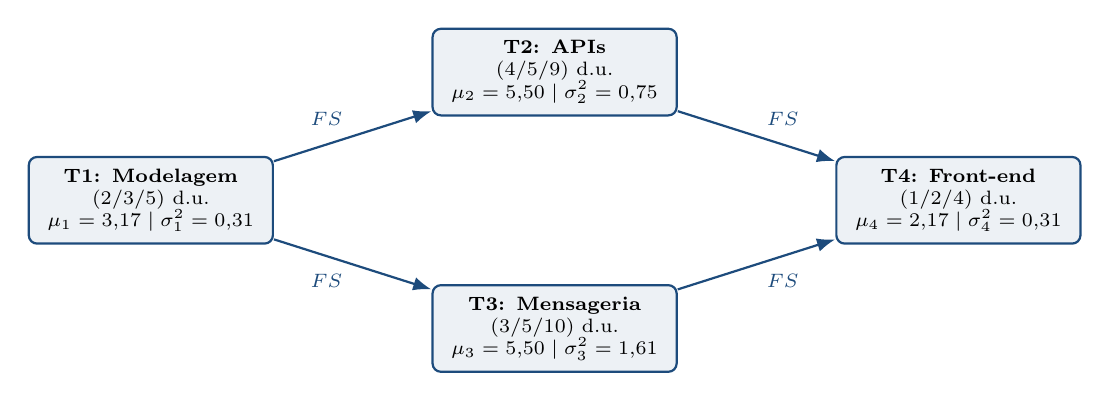
\begin{tikzpicture}[>=Latex, node distance=1.4cm and 2.4cm, every node/.style={font=\scriptsize}]
  \tikzstyle{task}=[rectangle, rounded corners=3pt, draw=unbblue, thick, fill=unbblue!8, minimum width=3.1cm, minimum height=1.1cm, align=center]
  \node[task] (t1) {\textbf{T1: Modelagem}\\$(2 / 3 / 5)$ d.u.\\$\mu_1 = 3{,}17 \mid \sigma_1^2 = 0{,}31$};
  \node[task, above right=0.5cm and 2.0cm of t1] (t2) {\textbf{T2: APIs}\\$(4 / 5 / 9)$ d.u.\\$\mu_2 = 5{,}50 \mid \sigma_2^2 = 0{,}75$};
  \node[task, below right=0.5cm and 2.0cm of t1] (t3) {\textbf{T3: Mensageria}\\$(3 / 5 / 10)$ d.u.\\$\mu_3 = 5{,}50 \mid \sigma_3^2 = 1{,}61$};
  \node[task, below right=0.5cm and 2.0cm of t2] (t4) {\textbf{T4: Front-end}\\$(1 / 2 / 4)$ d.u.\\$\mu_4 = 2{,}17 \mid \sigma_4^2 = 0{,}31$};
  \draw[->, thick, unbblue] (t1) -- node[above left]{$FS$} (t2);
  \draw[->, thick, unbblue] (t1) -- node[below left]{$FS$} (t3);
  \draw[->, thick, unbblue] (t2) -- node[above right]{$FS$} (t4);
  \draw[->, thick, unbblue] (t3) -- node[below right]{$FS$} (t4);
\end{tikzpicture}%
}

\section{Estimativa de Três Pontos e Distribuição PERT-Beta}\label{sec:pert}

Na Engenharia de Software, durações de tarefas e tempos de ciclo exibem forte assimetria positiva (cauda longa à direita) em razão de descobertas técnicas imprevistas, bloqueios externos e retrabalho de revisão \cite{maccrimmon1964,magennis2011,vacanti2015}. A técnica PERT clássica \cite{malcolm1959} parametriza a incerteza de cada atividade por três estimativas: otimista ($t_o$), mais provável ($t_m$) e pessimista ($t_p$), com $t_o \le t_m \le t_p$. Na formulação PERT modificada (\textit{Modified PERT}) difundida por \citeonline{vose2008} e \citeonline{davis2008}, a esperança matemática incorpora um parâmetro de peso modal $\lambda > 0$:
\begin{equation}\label{eq:pert_mean}
\mu_i=\frac{t_{o,i}+\lambda\,t_{m,i}+t_{p,i}}{\lambda+2},
\end{equation}
adotando-se como padrão $\lambda=4$, caso em que o PERT modificado coincide com a média clássica $\mu_i=(t_{o,i}+4t_{m,i}+t_{p,i})/6$.

Conforme demonstrado por \citeonline{maccrimmon1964}, a aproximação histórica da variância PERT clássica por $\sigma^2 \approx ((t_p-t_o)/6)^2$ introduz erros sistemáticos quando a moda $t_m$ se afasta do ponto médio do intervalo. Seguindo a parametrização exata da família PERT-Beta \cite{vose2008,davis2008}, este trabalho instancia diretamente a distribuição Beta contínua reescalada para o suporte compacto $[t_{o,i}, t_{p,i}]$. Para o caso não degenerado ($t_{p,i} - t_{o,i} > 0$), os parâmetros de forma $\alpha_i$ e $\beta_i$ são definidos por:
\begin{equation}\label{eq:pert_alpha_beta}
\alpha_i=1+\lambda\frac{t_{m,i}-t_{o,i}}{t_{p,i}-t_{o,i}},\qquad
\beta_i=1+\lambda\frac{t_{p,i}-t_{m,i}}{t_{p,i}-t_{o,i}},
\end{equation}
cuja soma é invariante ($\alpha_i+\beta_i=\lambda+2=6$ para $\lambda=4$). A variância analítica exata da variável reescalada $X_i = t_{o,i} + (t_{p,i}-t_{o,i})Y_i$, com $Y_i \sim \mathrm{Beta}(\alpha_i,\beta_i)$, é expressa por:
\begin{equation}\label{eq:pert_var}
\sigma_i^2=\frac{(\mu_i-t_{o,i})(t_{p,i}-\mu_i)}{\lambda+3} = \frac{(t_{p,i}-t_{o,i})^2\,\alpha_i\beta_i}{(\alpha_i+\beta_i)^2(\alpha_i+\beta_i+1)}.
\end{equation}
No caso limite degenerado em que $t_{o,i} = t_{m,i} = t_{p,i}$, define-se a distribuição como uma massa pontual determinística de Dirac em $t_{o,i}$, com $\mu_i = t_{o,i}$ e $\sigma_i^2 = 0$, evitando divisão por zero na Equação~\ref{eq:pert_alpha_beta}. A Figura~\ref{fig:pert} ilustra os perfis de densidade PERT-Beta das tarefas T1 a T4.

\figura{fig02_pert_beta.png}{Densidades PERT-Beta ($\lambda=4$) das tarefas T1 a T4; linhas verticais tracejadas indicam a moda $t_m$.}{fig:pert}{0.85}{%
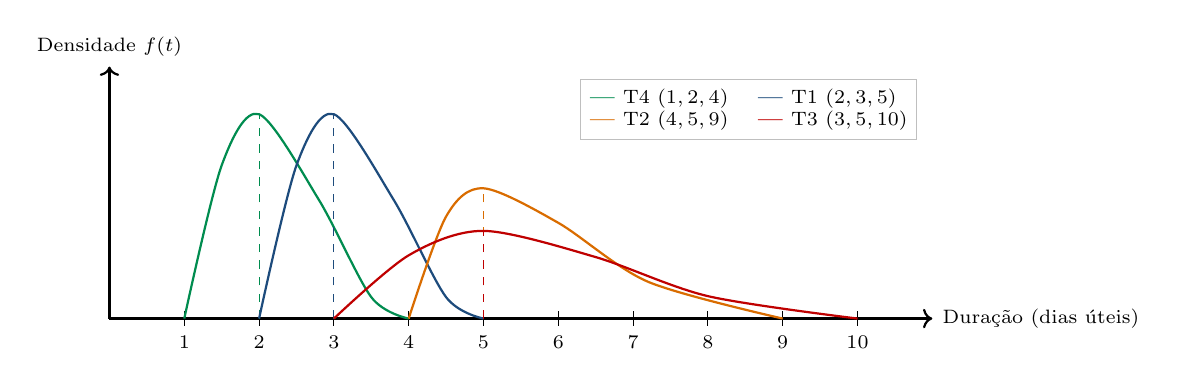
\begin{tikzpicture}[x=0.95cm,y=3.2cm, font=\scriptsize]
  \draw[->, thick] (0,0) -- (11,0) node[right]{Duração (dias úteis)};
  \draw[->, thick] (0,0) -- (0,1.00) node[above]{Densidade $f(t)$};
  \foreach \x in {1,2,3,4,5,6,7,8,9,10} \draw (\x,0.03) -- (\x,-0.03) node[below]{\x};
  % T4 (1,2,4): f(t_m=2) = 0.811
  \draw[thick, unbgreen] plot[smooth] coordinates {(1,0) (1.5,0.608) (2,0.811) (2.8,0.471) (3.5,0.085) (4,0)};
  \draw[dashed, unbgreen] (2,0) -- (2,0.811);
  % T1 (2,3,5): f(t_m=3) = 0.811
  \draw[thick, unbblue] plot[smooth] coordinates {(2,0) (2.5,0.608) (3,0.811) (3.8,0.471) (4.5,0.085) (5,0)};
  \draw[dashed, unbblue] (3,0) -- (3,0.811);
  % T2 (4,5,9): f(t_m=5) = 0.517
  \draw[thick, orange!85!black] plot[smooth] coordinates {(4,0) (4.5,0.405) (5,0.517) (6.0,0.380) (7.2,0.146) (9,0)};
  \draw[dashed, orange!85!black] (5,0) -- (5,0.517);
  % T3 (3,5,10): f(t_m=5) = 0.348
  \draw[thick, red!75!black] plot[smooth] coordinates {(3,0) (4.0,0.251) (5,0.348) (6.5,0.244) (8.0,0.089) (10,0)};
  \draw[dashed, red!75!black] (5,0) -- (5,0.348);
  % Legenda
  \node[anchor=north east, draw=gray!50, fill=white, align=left] at (10.8,0.95) {
    {\color{unbgreen}\textbf{---}} T4 $(1,2,4)$ \quad {\color{unbblue}\textbf{---}} T1 $(2,3,5)$\\
    {\color{orange!85!black}\textbf{---}} T2 $(4,5,9)$ \quad {\color{red!75!black}\textbf{---}} T3 $(3,5,10)$
  };
\end{tikzpicture}%
}

\section{Simulação de Monte Carlo e Viés de Convergência de Caminhos}\label{sec:montecarlo}

A aplicação do CPM sobre durações médias $\mu_i$ subestima sistematicamente o prazo final de redes com caminhos paralelos \cite{clark1961,vanslyke1963,hulett2000}. Em qualquer nó de convergência (\textit{join node}) com predecessoras paralelas $X_1,\dots,X_m$, o início da tarefa sucessora é governado pela estatística de ordem máxima $M = \max(X_1,\dots,X_m)$. Pela desigualdade de Jensen aplicada à função convexa máximo e pela formulação analítica dos momentos do máximo de variáveis aleatórias de \citeonline{clark1961}, tem-se:
\begin{equation}
E[\max(X_1,\dots,X_m)] \ge \max(E[X_1],\dots,E[X_m]),
\end{equation}
com desigualdade estrita sempre que os ramos tiverem suportes sobrepostos com variância positiva.

A Simulação de Monte Carlo resolve esse problema por integração estocástica em $N$ realizações independentes (adotando-se $N=10.000$) \cite{vanslyke1963,law2015}. Em cada iteração $k \in \{1,\dots,N\}$, para cada tarefa não concluída $i \in V$:
\begin{enumerate}
  \item Sorteia-se $Y_{i,k} = G_{1,k}/(G_{1,k}+G_{2,k})$, com variáveis $G_{1,k}\sim\mathrm{Gamma}(\alpha_i,1)$ e $G_{2,k}\sim\mathrm{Gamma}(\beta_i,1)$ geradas pelo método exato de rejeição de \citeonline{marsaglia2000};
  \item Calcula-se a duração base remanescente ponderada pelo progresso $c_i \in [0,1]$: $d_{i,k}^{\mathrm{base}} = (1-c_i)\,[t_{o,i} + (t_{p,i}-t_{o,i})Y_{i,k}]$;
  \item Somam-se as perturbações de riscos discretos $r \in \mathcal{R}_i$ modelados como ensaios de Bernoulli $B_{r,k}\sim\mathrm{Bernoulli}(p_r)$ com impacto remanescente $(1-c_i)\Delta_r$:
  \begin{equation}
  d_{i,k} = (1-c_i)\left[t_{o,i} + (t_{p,i}-t_{o,i})Y_{i,k} + \sum_{r\in\mathcal{R}_i} B_{r,k}\,\Delta_r\right];
  \end{equation}
  \item Executa-se o CPM sobre $\{d_{i,k}\}_{i\in V}$ a partir da data de status $t_s$, obtendo-se o término $F_k$ e as folgas $TF_{i,k}$.
\end{enumerate}

Da função de distribuição empírica $\hat{F}_N(t) = \frac{1}{N}\sum_{k=1}^N \mathbb{I}(F_k \le t)$ extraem-se a mediana $P_{50}$, o percentil de compromisso tático $P_{85}$, o percentil conservador $P_{95}$, a média amostral $\bar{F}$ e o Índice de Criticidade ($\IC_i$), formalizado na literatura de redes estocásticas por \citeonline{vanslyke1963} e \citeonline{williams1992}:
\begin{equation}
\IC_i=\frac{1}{N}\sum_{k=1}^{N}\mathbb{I}\left(|TF_{i,k}| \le \varepsilon\right)\times 100\%,
\end{equation}
que mede a probabilidade empírica de a atividade $i$ pertencer ao caminho crítico estocástico.

\section{Sombras Digitais, Gêmeos Digitais e Níveis de Maturidade}\label{sec:gemeos}

Originado na indústria aeroespacial e formalizado na manufatura pela norma ISO 23247-1 \cite{iso23247}, o paradigma de espelhamento digital foi categorizado por \citeonline{kritzinger2018} segundo o grau de automação do fluxo de dados entre o objeto físico (ou processo real) e sua contraparte virtual (Figura~\ref{fig:niveis}):

\begin{enumerate}
  \item \textbf{Modelo Digital (\textit{Digital Model}):} tanto a alimentação de dados do mundo real para o modelo quanto a aplicação de decisões do modelo no mundo real ocorrem de forma manual;
  \item \textbf{Sombra Digital (\textit{Digital Shadow}):} existe um fluxo de dados unidirecional automatizado do objeto real para o modelo virtual (sincronização contínua de estado), mas qualquer alteração de volta sobre o processo real exige decisão e ação humana;
  \item \textbf{Gêmeo Digital (\textit{Digital Twin}):} os fluxos de dados são bidirecionais e totalmente automatizados, permitindo que o modelo virtual altere parâmetros do sistema real sem intervenção humana contínua.
\end{enumerate}

\figuraAdaptada{fig03_niveis_gemeo_digital.png}{Níveis de integração e maturidade segundo \citeonline{kritzinger2018} e posicionamento do artefato como Sombra Digital Governada.}{fig:niveis}{0.85}{%
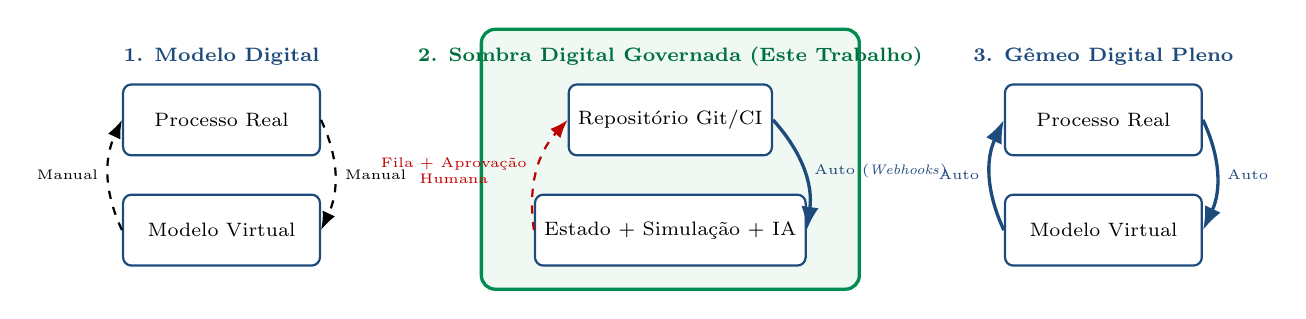
\begin{tikzpicture}[>=Latex, font=\scriptsize, every node/.style={align=center}]
  \tikzstyle{box}=[rectangle, rounded corners=3pt, draw=unbblue, thick, fill=white, minimum width=2.5cm, minimum height=0.9cm]
  % 1. Modelo Digital
  \node[font=\bfseries\scriptsize, unbblue] at (0, 1.5) {1. Modelo Digital};
  \node[box] (f1) at (0, 0.7) {Processo Real};
  \node[box] (v1) at (0, -0.7) {Modelo Virtual};
  \draw[->, dashed, thick] (f1.east) to[bend left=25] node[right, font=\tiny]{Manual} (v1.east);
  \draw[->, dashed, thick] (v1.west) to[bend left=25] node[left, font=\tiny]{Manual} (f1.west);
  % 2. Sombra Digital Governada
  \draw[rounded corners=5pt, draw=unbgreen, very thick, fill=unbgreen!6] (3.3,-1.45) rectangle (8.1,1.85);
  \node[font=\bfseries\scriptsize, unbgreen!80!black] at (5.7, 1.5) {2. Sombra Digital Governada (Este Trabalho)};
  \node[box] (f2) at (5.7, 0.7) {Repositório Git/CI};
  \node[box] (v2) at (5.7, -0.7) {Estado + Simulação + IA};
  \draw[->, very thick, unbblue] (f2.east) to[bend left=25] node[right, font=\tiny]{Auto (\textit{Webhooks})} (v2.east);
  \draw[->, dashed, thick, red!75!black] (v2.west) to[bend left=25] node[left, font=\tiny]{Fila + Aprovação\\Humana} (f2.west);
  % 3. Gemeo Digital
  \node[font=\bfseries\scriptsize, unbblue] at (11.2, 1.5) {3. Gêmeo Digital Pleno};
  \node[box] (f3) at (11.2, 0.7) {Processo Real};
  \node[box] (v3) at (11.2, -0.7) {Modelo Virtual};
  \draw[->, very thick, unbblue] (f3.east) to[bend left=25] node[right, font=\tiny]{Auto} (v3.east);
  \draw[->, very thick, unbblue] (v3.west) to[bend left=25] node[left, font=\tiny]{Auto} (f3.west);
\end{tikzpicture}%
}{\citeonline{kritzinger2018}}

Na Engenharia de Software, o objeto monitorado é um processo sociotécnico composto por desenvolvedores, repositórios de código, \textit{pipelines} de CI/CD e artefatos de planejamento \cite{guinea2024,lehner2025}. Embora parte da literatura empregue o termo guarda-chuva ``Gêmeo Digital de Processo'' para qualquer representação sincronizada, adotar atuação reversa totalmente automatizada (nível 3 de Kritzinger) quando há um agente LLM no laço decisório representaria uma vulnerabilidade crítica de governança, pois uma alucinação ou um ataque de injeção poderia reescrever prazos contratuais, dependências ou tarefas no repositório sem supervisão.

Por essa razão, este trabalho adota o enquadramento rigoroso de \textbf{Sombra Digital Governada de Processo}: a ingestão de eventos do GitHub/CI para o modelo virtual é 100\% automatizada e idempotente, a IA pode acionar autonomamente apenas simulações transitórias em memória e rascunhos isolados (Categoria 1), e toda mutação sobre a linha de base ou sobre o grafo oficial requer aprovação humana explícita apoiada por simulação de impacto (Categoria 2).

\section{Vulnerabilidades e Governança de Agentes Baseados em LLM}\label{sec:owasp}

A integração de agentes baseados em LLMs a sistemas corporativos introduz vetores de ataque específicos, sistematizados pelo projeto OWASP Top 10 for LLM Applications em sua versão 1.1 \cite{owasp2023} e atualizados na edição 2025 \cite{owasp2025}, em alinhamento com o referencial de gestão de risco NIST AI RMF 1.0 \cite{nist2023}. A fim de evitar ambiguidades taxonômicas entre as duas edições do OWASP, este trabalho harmoniza explicitamente a numeração de ambas para os cinco riscos tratados pela arquitetura:

\begin{itemize}
  \item \textbf{Injeção de Prompt (\texttt{LLM01} em 2023 e 2025):} ocorre de forma indireta quando o LLM processa textos provenientes de fontes externas não confiáveis — tais como títulos de \textit{issues} ou resumos de \textit{pull requests} criados por terceiros — contendo instruções adversariais ocultas que tentam subverter o \textit{prompt} de sistema \cite{greshake2023,debenedetti2024};
  \item \textbf{Divulgação de Informações Sensíveis (\texttt{LLM06} na v1.1 de 2023; reclassificada como \texttt{LLM02} na edição 2025):} exposição indevida de dados pessoais (PII), segredos, credenciais ou propriedade intelectual enviados sem filtragem ao provedor externo do modelo de linguagem;
  \item \textbf{Tratamento Inseguro de Saída (\texttt{LLM02} na v1.1 de 2023; reclassificada como \texttt{LLM05} na edição 2025 — \textit{Improper Output Handling}):} renderização ou execução de respostas do LLM sem codificação contextual, sanitização estrita de marcação HTML/Markdown ou validação estrutural de esquema, abrindo brechas para \textit{Cross-Site Scripting} (XSS) na interface do aprovador;
  \item \textbf{Agência Excessiva (\texttt{LLM08} na v1.1 de 2023; reclassificada como \texttt{LLM06} na edição 2025):} concessão de permissões excessivas, ferramentas irrestritas ou acesso direto de escrita ao banco de dados para um componente probabilístico, permitindo que falhas de raciocínio ou comandos injetados desencadeiem ações destrutivas;
  \item \textbf{Consumo Ilimitado / Negação de Serviço (\texttt{LLM04} na v1.1 de 2023; ampliada como \texttt{LLM10} na edição 2025 — \textit{Unbounded Consumption}):} exaustão de recursos computacionais ou de orçamento de API quando rajadas de eventos externos disparam chamadas síncronas ou recursivas ao provedor de LLM sem controle de taxa (\textit{rate limiting}) e teto de \textit{tokens}.
\end{itemize}

Na literatura recente de defesa arquitetural para agentes LLM, \citeonline{debenedetti2025camel} (sistema CaMeL) e \citeonline{beurerkellner2025patterns} demonstram que filtros puramente heurísticos sobre prompts são insuficientes contra injeções adaptativas, recomendando a separação estrita entre fluxos de controle e fluxos de dados não confiáveis, aliada à validação determinística de capacidades fora do modelo. Além da execução direta de comandos, sistemas com aprovação humana (\textit{human-in-the-loop}) estão sujeitos à ameaça de \textbf{persuasão cognitiva do aprovador}: um texto adversarial injetado pode induzir o LLM a redigir uma justificativa aparentemente técnica para convencer o gerente humano a aprovar uma alteração danosa no cronograma. Embora o desenho de interface com segregação visual entre métricas determinísticas e texto não verificado reduza a confusão visual, ele não elimina o viés de automação humano, exigindo travas estruturais adicionais no servidor detalhadas na Seção~\ref{sec:ameacas_ia}.

\section{Trabalhos Relacionados}

A Tabela~\ref{tab:relacionados} sintetiza os estudos que fundamentam o estado da arte nos quatro eixos da pesquisa: Sombras/Gêmeos Digitais na Engenharia de Software, simulação estocástica e predição de atrasos em cronogramas (baseada em rede PERT-Beta, em vazão Kanban e em aprendizado de máquina) e segurança de agentes LLM.

\begin{table}[htbp]
\caption{Trabalhos relacionados: análise comparativa de abordagens e lacunas.}\label{tab:relacionados}
\footnotesize
\begin{tabularx}{\textwidth}{L{2.5cm} L{2.4cm} L{2.2cm} L{1.4cm} Y}
\toprule
\textbf{Trabalho} & \textbf{Foco} & \textbf{Abordagem} & \textbf{IA} & \textbf{Limitações observadas}\\
\midrule
\citeonline{guinea2024} & Revisão sistemática de gêmeos digitais em Eng. Software & Qualitativa/conceitual & Não & Não propõe arquitetura executável nem motor estocástico verificado\\
\citeonline{lehner2025} & Mapeamento de MDE aplicado a gêmeos digitais & Mapeamento (66 de 189 estudos) & Não & Foco em sistemas ciberfísicos; não modela cronogramas de software\\
\citeonline{hulett2000} & Risco quantitativo em cronogramas & Monte Carlo \textit{vs.} PERT & Não & Sem sincronização contínua por eventos Git/CI nem camada de IA\\
\citeonline{vanslyke1963} & Monte Carlo em redes PERT & Simulação de caminhos paralelos & Não & Processamento em lote estático; sem progresso parcial nem governança\\
\citeonline{vacanti2015} & Previsão de fluxo em sistemas Kanban & Monte Carlo por vazão histórica & Não & Ignora topologia de dependências $FS$ e riscos discretos por tarefa\\
\citeonline{choetkiertikul2018} & Predição de entrega em desenvolvimento iterativo & Aprendizado de máquina sobre \textit{issues} & ML preditivo & Estima risco por item/iteração sem modelar rede $FS$ explícita nem governança de agentes LLM\\
\citeonline{jorgensen2004} & Estimativas de esforço em software & Revisão de estudos empíricos & Não & Diagnóstico de vieses humanos; não oferece motor de simulação\\
\citeonline{greshake2023} & Injeção indireta de \textit{prompt} & Análise empírica de ataques & Agentes LLM & Demonstra a superfície de ataque; não formaliza motor determinístico isolado\\
\citeonline{debenedetti2024} & \textit{Benchmark} AgentDojo (NeurIPS 2024) & Avaliação de ataques e defesas & Agentes LLM & Ambiente genérico de ferramentas; não trata governança de cronogramas\\
\textbf{Este trabalho} & Sombra Digital Governada para cronogramas & CPM + Monte Carlo (PERT-Beta + Bernoulli) & LLM isolado (\textit{fail-closed}) & Planejamento tático com dependências $FS$; capacidade de recursos infinita no MVP\\
\bottomrule
\end{tabularx}
\fonteautores
\end{table}

Observa-se na Tabela~\ref{tab:relacionados} uma complementaridade entre três vertentes da literatura: estudos de Pesquisa Operacional \cite{clark1961,vanslyke1963,williams1992,hulett2000} modelam a topologia da rede e o viés de convergência, mas operam desconectados dos repositórios de código; métodos ágeis probabilísticos \cite{magennis2011,vacanti2015} e preditores baseados em aprendizado de máquina sobre artefatos de \textit{issues} \cite{choetkiertikul2018} exploram dados históricos de repositórios, porém não propagam incertezas sobre grafos explícitos de precedência $FS$ nem oferecem simulação \textit{what-if} de caminhos críticos; já os estudos de segurança em IA \cite{greshake2023,debenedetti2024,debenedetti2025camel,beurerkellner2025patterns} evidenciam a fragilidade de agentes autônomos, motivando o isolamento arquitetural proposto.

\section{Matriz Comparativa de Ferramentas Existentes}

A Tabela~\ref{tab:ferramentas} compara soluções comerciais utilizadas em 2026 — incluindo ferramentas ágeis/ALM e suítes dedicadas de análise quantitativa de risco em cronogramas — com o artefato proposto neste trabalho. Para garantir transparência quanto ao estágio atual do projeto (conclusão do TCC1), a linha referente a este trabalho separa explicitamente as capacidades já \textbf{Verificadas em PoC (TCC1)} daquelas \textbf{Projetadas para implementação integradora no TCC2}.

\begin{table}[htbp]
\caption{Matriz comparativa entre ferramentas existentes no mercado (estado em out. 2026) e o artefato proposto.}\label{tab:ferramentas}
\scriptsize
\begin{tabularx}{\textwidth}{L{2.5cm} Y Y Y Y Y Y}
\toprule
\textbf{Ferramenta} & \textbf{Sinc. Git/CI} & \textbf{CPM e Folgas} & \textbf{Monte Carlo} & \textbf{\textit{What-if}} & \textbf{IA e Governança} & \textbf{Auditoria}\\
\midrule
Jira Cloud Plans + Atlassian Rovo$^1$ & Alta (nativa/apps) & Parcial (Gantt determinístico) & Não nativo (exige \textit{plugins} pagos) & Limitado (planos visuais) & Agente Rovo (sem \textit{fail-closed} sob grafo estocástico) & Log relacional administrativo\\
Azure DevOps + GitHub Copilot$^2$ & Alta (nativa) & Limitado (\textit{Delivery Plans} sem $TF_i$) & Não nativo & Não & Copilot assistivo (sem isolamento de rede dedicado) & Log padrão de auditoria\\
LiquidPlanner$^3$ & Baixa (via conectores) & Sim & Sim (intervalos por tarefa) & Parcial & Sem agente LLM governado & Log padrão relacional\\
ActionableAgile / Nave$^4$ & Média (importa estados) & Não (agnóstico a DAG $FS$) & Sim (apenas por vazão histórica) & Sim (ajuste de vazão) & Sem agente LLM governado & Histórico da plataforma host\\
Primavera Risk Analysis / Acumen Risk / @RISK$^5$ & Nula (importação manual XER/MPP) & Sim (CPM completo e $\IC_i$) & Sim (PERT-Beta, correlações e eventos) & Sim (cenários completos) & Sem agente LLM governado nem \textit{allowlist} & Log de arquivos/banco corporativo\\
\textbf{Artefato proposto} & \textbf{Projetado (TCC2):} \textit{webhooks} HMAC idempotentes & \textbf{Verificado em PoC (TCC1):} CPM exato e $TF_i$ & \textbf{Verificado em PoC (TCC1):} PERT-Beta + Bernoulli & \textbf{Verificado em PoC / Persistência no TCC2} & \textbf{Projetado (TCC2):} LLM em sub-rede isolada + \textit{fail-closed} & \textbf{Projetado (TCC2):} SHA-256 \textit{tamper-evident} + âncora\\
\bottomrule
\end{tabularx}
\par\vspace{1mm}{\tiny Fontes técnicas consultadas em 20 out. 2026: $^1$Atlassian Plans Dependency Management \& Rovo Agent Security (\url{https://support.atlassian.com/jira-software-cloud/docs/manage-dependencies-in-advanced-roadmaps/}); $^2$Microsoft Azure Boards Delivery Plans (\url{https://learn.microsoft.com/en-us/azure/devops/boards/plans/review-team-plans}); $^3$LiquidPlanner Predictive Scheduling Engine (\url{https://www.liquidplanner.com/features/predictive-scheduling/}); $^4$ActionableAgile Monte Carlo Forecasting (\url{https://www.55degrees.se/products/actionableagile}); $^5$Oracle Primavera Risk Analysis User's Guide (\url{https://docs.oracle.com/cd/E51302_01/help/en/helpmain.htm}) e Deltek Acumen Risk Documentation.}
\end{table}

Conforme sintetizado na Tabela~\ref{tab:ferramentas}, ferramentas como Jira e Azure DevOps incorporaram assistentes baseados em LLMs até 2026 (Atlassian Rovo e GitHub Copilot), mas permanecem desprovidas de simulação de Monte Carlo nativa acoplada ao grafo de dependências e não oferecem retenção de mutações condicionada à visualização prévia de deslocamentos de percentis ($\Delta P_{50}, \Delta P_{85}$) calculados por um motor estocástico determinístico.

% =====================================================================
\chapter{Metodologia}\label{cap:metodologia}
% =====================================================================

Este capítulo descreve o método científico adotado para especificar, verificar em Prova de Conceito e planejar a avaliação empírica da arquitetura proposta. A pesquisa classifica-se como aplicada, de objetivos explicativos e prescritivos, abordagem quantitativa e conduzida sob a \textit{Design Science Research Methodology} (DSRM) \cite{peffers2007}.

\section{Enquadramento nas Seis Atividades da DSRM}\label{sec:dsrm}

Para assegurar rastreabilidade metodológica entre o problema prático e as entregas do TCC1 e do TCC2, o trabalho estrutura-se explicitamente ao longo das seis atividades canônicas propostas por \citeonline{peffers2007}, sintetizadas na Tabela~\ref{tab:dsrm}.

\begin{table}[htbp]
\caption{Mapeamento das seis atividades da DSRM no ciclo da pesquisa (TCC1 e TCC2).}\label{tab:dsrm}
\footnotesize
\begin{tabularx}{\textwidth}{L{2.8cm} L{1.6cm} Y Y}
\toprule
\textbf{Atividade DSRM} & \textbf{Etapa} & \textbf{Realização na pesquisa} & \textbf{Seções / Entregáveis}\\
\midrule
1. Identificação do problema e motivação & TCC1 (Concluída) & Caracterização da desconexão entre eventos Git/CI e modelos formais de rede, do viés de convergência em caminhos paralelos e das vulnerabilidades de LLMs não governados (OWASP LLM01, LLM02, LLM05, LLM06 e LLM10) & Cap.~\ref{cap:introducao} e Cap.~\ref{cap:revisao}\\
2. Definição dos objetivos da solução & TCC1 (Concluída) & Formulação de RQ1 a RQ4, das hipóteses H1a, H1b, H2a e H2b, dos critérios CA1 e CA2 e dos requisitos verificáveis RF01--RF12 e RNF01--RNF09 & Seção~\ref{sec:requisitos} (Tabelas~\ref{tab:rf} e \ref{tab:rnf})\\
3. Projeto e desenvolvimento (\textit{Design \& Development}) & TCC1 (Arquitetura + Motor PoC) e TCC2 (MVP) & Especificação da arquitetura proposta da Sombra Digital Governada, implementação do motor estocástico em Go (\texttt{poc-engine}) no TCC1 e integração dos serviços no TCC2 & Cap.~\ref{cap:arquitetura} e Cap.~\ref{cap:poc}\\
4. Demonstração & TCC1 (PoC) e TCC2 (Sistema) & Execução do motor nos cenários A, B, C e C$'$ e no cronograma do TCC2, extração do repositório \texttt{cli/cli} no TCC1 e demonstração ponta a ponta no TCC2 & Seções~\ref{sec:backtesting}, \ref{sec:poc_cenarios} e \ref{sec:sim_tcc2}\\
5. Avaliação (\textit{Evaluation}) & TCC1 (Dim. 1) e TCC2 (Dim. 2--5) & Verificação analítica, teste KS, MCSE, reprodutibilidade multi-\textit{worker} e \textit{benchmark} no TCC1 (Dim. 1); calibração sintética em 10 regimes ($M=200$), \textit{backtesting} descritivo, segurança adversarial e ablação da IA no TCC2 (Dim. 2--5) & Seção~\ref{sec:protocolo} (Tabela~\ref{tab:protocolo}) e Cap.~\ref{cap:poc}\\
6. Comunicação & TCC1 e TCC2 & Monografia de TCC1, repositório público versionado com pacote de replicação pseudonimizado, \textit{scripts} auditáveis e defesa pública final no TCC2 & Apêndices~\ref{apd:mvp} e \ref{apd:extracao}\\
\bottomrule
\end{tabularx}
\fonteautores
\end{table}

\section{Requisitos do Sistema}\label{sec:requisitos}

A elicitação de requisitos decorre diretamente das questões de pesquisa RQ1 a RQ4 e dos controles de segurança discutidos na Seção~\ref{sec:owasp}. Os Requisitos Funcionais (RF01 a RF12), detalhados na Tabela~\ref{tab:rf}, abrangem o ciclo completo da Sombra Digital Governada: cadastro estrutural de projetos, papéis, Estrutura Analítica do Projeto (WBS), tarefas com estimativas de três pontos e riscos discretos (RF01 e RF02); ingestão idempotente de eventos GitHub/CI e controle monotônico de versão de estado com \textit{debounce} (RF03 e RF04); execução do CPM e da Simulação de Monte Carlo (RF05 e RF06); recomendação interpretativa por IA isolada submetida a classificação binária determinística no servidor e fila de aprovação com pré-visualização de impacto (RF07, RF08 e RF09); trilha de auditoria encadeada (RF10); interface web mínima reativa (RF11); e emissão de alertas determinísticos independentes da IA (RF12).

\begin{table}[htbp]
\caption{Requisitos Funcionais do sistema (RF01 a RF12).}\label{tab:rf}
\footnotesize
\begin{tabularx}{\textwidth}{L{1cm} L{3.9cm} Y L{1.1cm}}
\toprule
\textbf{ID} & \textbf{Requisito} & \textbf{Descrição detalhada} & \textbf{Prior.}\\
\midrule
RF01 & Cadastrar projetos e membros & CRUD de projetos, marcos (\textit{releases}) e membros com controle de papéis (Gerente, Membro) & Alta\\
RF02 & Cadastrar WBS, tarefas e riscos & CRUD de pacotes WBS, tarefas com $(t_o,t_m,t_p)$, dependências $FS$ acíclicas e riscos discretos com $(p_r, \Delta_r)$ & Alta\\
RF03 & Ingestão idempotente de eventos & Recepção de eventos manuais e \textit{webhooks} GitHub validados por assinatura HMAC-SHA256 e chave de entrega & Alta\\
RF04 & Manter estado versionado & Contador monotônico \texttt{state\_version} separado da linha de base oficial, com janela de \textit{debounce} de 30 s & Alta\\
RF05 & Calcular caminho crítico & Execução determinística do CPM ($ES_i, EF_i, LS_i, LF_i, TF_i$) a partir da data de status $t_s$ & Alta\\
RF06 & Executar Simulação de Monte Carlo & Amostragem concorrente PERT-Beta + Bernoulli com persistência de cenários hipotéticos em \texttt{JSONB} & Alta\\
RF07 & Agente de IA para apoio à decisão & Serviço isolado que consome a \textit{allowlist} sob gatilho condicional e emite recomendações em JSON Schema estrito & Alta\\
RF08 & Classificação determinística (\textit{fail-closed}) & Validação no servidor que classifica ações em Categoria 1 (Autônoma) ou Categoria 2 (Restrita) e nega por padrão qualquer tipo desconhecido & Alta\\
RF09 & Fila de aprovação com impacto simulado & Retenção de ações de Categoria 2 até decisão do Gerente, exibindo $\Delta P_{50}$, $\Delta P_{85}$, $\Delta P_{95}$ e $\Delta\IC_i$ em painel segregado com subfluxos CRN & Alta\\
RF10 & Trilha de auditoria resistente a adulterações & Registro encadeado por SHA-256 de eventos, sugestões e decisões, com ancoragem externa periódica do \textit{hash} de cabeça & Alta\\
RF11 & Interface mínima reativa & SPA exibindo tabela do caminho crítico, curvas de distribuição acumulada e fila de aprovação governada & Média\\
RF12 & Alertas determinísticos de limiar & Disparo automático de alertas no \textit{Core} quando $P_{85}$ ultrapassa a meta do marco ou $\IC_i$ supera limiar configurado, sem depender do LLM & Alta\\
\bottomrule
\end{tabularx}
\fonteautores
\end{table}

De forma complementar, a Tabela~\ref{tab:rnf} especifica os nove Requisitos Não Funcionais (RNF01 a RNF09) e seus respectivos critérios objetivos de aceitação e verificação experimental. Destaca-se a articulação entre o RNF01 (autenticação JWT e autorização RBAC estrita nas rotas de decisão), o RNF02 (minimização de dados via \textit{allowlist} sanitizada), o RNF03 (auditoria \textit{tamper-evident} ancorada), o RNF04 e o RNF07 (defesa em profundidade contra injeção de \textit{prompt}, sanitização de saída e isolamento de sub-rede Docker), além das metas de desempenho desacopladas entre motor e ciclo ponta a ponta (RNF06) e reprodutibilidade determinística em função do índice de iteração (RNF08).

\begin{table}[htbp]
\caption{Requisitos Não Funcionais do sistema (RNF01 a RNF09).}\label{tab:rnf}
\footnotesize
\begin{tabularx}{\textwidth}{L{1.2cm} L{4.0cm} Y}
\toprule
\textbf{ID} & \textbf{Requisito} & \textbf{Critério objetivo de aceitação e método de verificação}\\
\midrule
RNF01 & Controle de acesso por papéis (RBAC) & Autenticação via JWT assinado; retorno obrigatório \texttt{403 Forbidden} caso usuários com papel Membro ou o serviço de IA invoquem rotas de aprovação (Cat. 2)\\
RNF02 & Privacidade e minimização (\textit{Allowlist}) & Envio exclusivo do contrato JSON da \textit{allowlist} ao LLM (métricas numéricas e títulos sanitizados truncados); bloqueio total de PII, e-mails, código-fonte e corpos de \textit{commit}\\
RNF03 & Auditoria \textit{tamper-evident} ancorada & Revogação de \texttt{UPDATE}/\texttt{DELETE} para o usuário da aplicação em \texttt{audit\_logs}, \textit{trigger} de bloqueio, cadeia SHA-256 e exportação do \texttt{head\_hash} para repositório externo \textit{append-only}\\
RNF04 & Defesa estrutural contra \textit{prompt injection} e XSS & Zero mutações não autorizadas sob bateria de \textit{payloads} adversariais, rejeição \textit{fail-closed}, renderização em texto puro e cabeçalho CSP estrito na interface\\
RNF05 & Consistência e idempotência & Restrições \texttt{UNIQUE} em \texttt{delivery\_id} e \texttt{idempotency\_key}; marcação \texttt{is\_stale = true} para simulações cujo \texttt{base\_state\_version} divergir do estado atual\\
RNF06 & Desempenho do motor e ciclo síncrono & (i) Motor em memória: $N=10.000$ iterações em mediana $< 500$ ms para redes de até 200 tarefas e 300 dependências; (ii) Ciclo síncrono ponta a ponta (HTTP + fila SQL + \textit{worker} + persistência + SSE, excluindo LLM externo): $P_{95} < 2{,}0$ s\\
RNF07 & Isolamento físico, de rede e de cota da IA & Contêiner de IA exclusivo na rede \texttt{ai-isolated-net}, sem rota SQL, com \textit{rate limiting} (6 chamadas/min), orçamento de \textit{tokens} e disparo condicional por limiar de relevância\\
RNF08 & Reprodutibilidade determinística por índice & Mesma rede de entrada e semente $S_0$ produzem quantis, média compensada de Kahan e $\IC_i$ idênticos em \texttt{float64} com 1, 4 ou 16 \textit{workers}\\
RNF09 & Explicabilidade e verificação numérica & Toda recomendação referencia \texttt{scenario\_id} e indicadores da \textit{allowlist}; verificador determinístico valida literais numéricos conforme a precisão de casas decimais citada ($\pm 0{,}05$ para 1 casa decimal; $\pm 0{,}01$ para 2 casas decimais)\\
\bottomrule
\end{tabularx}
\fonteautores
\end{table}

\section{Caracterização Empírica das Janelas de \textit{Backtesting}}\label{sec:backtesting}

\subsection{Fonte, Definição Operacional e Extração Reprodutível}

Para investigar a aplicabilidade do modelo sobre dados reais de engenharia de software (Dimensão 3 da avaliação), selecionou-se o repositório oficial do GitHub CLI (\texttt{cli/cli}), projeto de código aberto mantido em Go cujo histórico de \textit{issues}, \textit{pull requests} e \textit{releases} é integralmente público. A coleta auditável no TCC1 foi realizada pelo \textit{script} \texttt{extract\_dataset.py} (documentado no Apêndice~\ref{apd:extracao}), combinando a API REST pública do GitHub e o histórico Git do repositório:

\begin{itemize}
  \item \textbf{Janela de \textit{release}:} intervalo temporal entre a publicação da \textit{release} imediatamente anterior e a da \textit{release}-alvo (v2.39.2 em 27/11/2023; v2.40.0 em 07/12/2023; v2.41.0 em 08/01/2024; v2.46.0 em 20/03/2024);
  \item \textbf{Filtragem de itens e motivos de fechamento:} são extraídos os PRs mesclados (\texttt{merged\_at != null}) na janela, descartando contas automáticas (\texttt{Dependabot}, \texttt{github-actions}), contabilizando separadamente os PRs fechados sem \textit{merge} (\texttt{is:unmerged}) e as \textit{issues} encerradas com razão \texttt{state\_reason = completed} (separadas de \texttt{not\_planned});
  \item \textbf{Contraste entre tempo de revisão do PR e duração de engenharia:} a função \texttt{business\_days} mede dias úteis fracionários em escala contínua de 24 horas por dia útil (segunda a sexta-feira). Para demonstrar empiricamente a diferença de construto, o \textit{script} extrai tanto o tempo de revisão do PR ($\texttt{merged\_at} - \texttt{created\_at}_{\mathrm{PR}}$) quanto a duração de engenharia corrigida desde o primeiro \textit{commit} da \textit{branch} ($\max(0{,}25;\; \texttt{merged\_at} - \min(\texttt{first\_commit\_at}, \texttt{created\_at}_{\mathrm{PR}}))$);
  \item \textbf{Pseudonimização e proteção de dados (LGPD/GDPR):} o extrator descarta integralmente logins de usuários (\texttt{user.login}), nomes civis e endereços de e-mail, persistindo apenas contagens agregadas, durações numéricas e rótulos técnicos (\texttt{dataset\_backtesting.json});
  \item \textbf{Vínculo PR--\textit{issue}:} identificado por expressões regulares sobre palavras-chave de fechamento (\texttt{closes}, \texttt{fixes}, \texttt{resolves}) seguidas do identificador numérico da \textit{issue}.
\end{itemize}

\subsection{Análise dos Dados Extraídos, Variável-Alvo e Parametrização Causal}

A Tabela~\ref{tab:backtesting} sintetiza as métricas obtidas para três recortes temporais do repositório \texttt{cli/cli}: duas janelas unitárias de \textit{release} (Casos 1 e 2) e uma janela agregada de um trimestre (v2.40.0 a v2.46.0).

\begin{table}[htbp]
\caption{Caracterização quantitativa de janelas de \textit{release} do GitHub CLI (\texttt{cli/cli}) para \textit{backtesting}.}\label{tab:backtesting}
\footnotesize
\begin{tabularx}{\textwidth}{L{5.0cm} Y Y Y}
\toprule
\textbf{Métrica observada} & \textbf{Caso 1: v2.40.0} & \textbf{Caso 2: v2.41.0} & \textbf{Ampliada: v2.40.0 $\rightarrow$ v2.46.0}\\
\midrule
Intervalo calendário & 27/11/2023 $\rightarrow$ 07/12/2023 & 07/12/2023 $\rightarrow$ 08/01/2024 & 07/12/2023 $\rightarrow$ 20/03/2024\\
Duração da janela (dias úteis) & 7,88 & 21,97 & 74,08\\
PRs mesclados (total / sem \textit{bots}) & 11 / 11 & 16 / 13 & 72 / 62\\
PRs fechados sem \textit{merge} (excluídos) & 3 & 6 & 28\\
PRs com vínculo explícito a \textit{issue} & 6 (55\%) & 6 (46\%) & 32 (52\%)\\
PRs com 1º \textit{commit} anterior ao PR & 7 (64\%) & 12 (92\%) & 45 (73\%)\\
\textit{Issues} concluídas (\texttt{completed} / \texttt{not\_planned}) & 10 / 1 & 19 / 3 & 92 / 8\\
Revisão PR ($\texttt{created}\rightarrow\texttt{merged}$) P10 / P50 / P90 (d.u.) & 0,01 / 2,43 / 9,59 & 0,01 / 0,06 / 4,19 & 0,01 / 1,11 / 28,99\\
Revisão PR --- Média (d.u.) & 3,88 & 2,07 & 9,45\\
Duração Eng. (desde 1º \textit{commit}) P10 / P50 / P90 (d.u.) & 0,25 / 4,54 / 15,32 & 0,25 / 0,25 / 4,20 & 0,25 / 1,11 / 29,00\\
Duração Eng. (desde 1º \textit{commit}) --- Média (d.u.) & 7,36 & 2,21 & 9,59\\
\bottomrule
\end{tabularx}
{\small Fonte: Extração própria auditável (\texttt{extract\_dataset.py --verify-local} e \texttt{dataset\_backtesting.json}).}
\end{table}

A inspeção da Tabela~\ref{tab:backtesting} fundamenta cinco definições metodológicas para o protocolo de \textit{backtesting} do TCC2:

\begin{enumerate}
  \item \textbf{Correção da validade de construto (\textit{PR review time} vs. duração desde o 1º \textit{commit}):} no Caso 2, a mediana ($P_{50}$) do tempo entre abertura e \textit{merge} do PR é de $0{,}06$ d.u. (equivalente a $0{,}06 \times 24\text{ h} \approx 1{,}45\text{ h}$ na convenção de dias úteis contínuos de 24h do extrator, ou $\approx 0{,}48\text{ h}$ em jornada comercial de 8h). Além disso, entre 64\% e 92\% dos PRs possuem \textit{commits} anteriores à abertura do PR: no Caso 1 (\texttt{v2.40.0}), incorporar o histórico desde o primeiro \textit{commit} eleva a mediana de $2{,}43$ d.u. para $4{,}54$ d.u., o $P_{90}$ de $9{,}59$ d.u. para $15{,}32$ d.u. e a média de $3{,}88$ d.u. para $7{,}36$ d.u. Assim, a duração operacional de cada tarefa $i$ é definida por $d_i = \max(0{,}25;\; \texttt{merged\_at}_i - \min(\texttt{first\_commit\_at}_i, \texttt{issue\_assigned\_at}_i, \texttt{pr\_created\_at}_i))$;
  \item \textbf{Definição formal da variável-alvo $y$ e controle de \textit{scope creep}:} como projetos de código aberto podem publicar \textit{releases} por cadência ou incorporar itens emergenciais após um ponto de corte temporal $t_c$, avaliam-se duas variáveis-alvo complementares para cada janela de \textit{release}:
  \begin{equation}
  y_{\mathrm{congelado}}(t_c) = \max_{i \in S(t_c)} \left(t_{\mathrm{fim},i} - t_{\text{início,marco}}\right), \qquad y_{\mathrm{release}} = t_{\mathrm{tag}} - t_{\text{início,marco}},
  \end{equation}
  onde $S(t_c)$ é o conjunto de tarefas do marco já abertas ou conhecidas até o instante $t_c$. A métrica primária de acurácia do simulador é calculada sobre $y_{\mathrm{congelado}}(t_c)$ (isolando a capacidade preditiva sobre o escopo conhecido em $t_c$), enquanto a razão de inflação de escopo $\rho_{\mathrm{escopo}}(t_c) = |S(T) \setminus S(t_c)| / |S(t_c)|$ e o erro contra $y_{\mathrm{release}}$ são reportados separadamente;
  \item \textbf{Regra causal de parametrização $(t_o, t_m, t_p)$ por casamento de quantis e agrupamento hierárquico:} em qualquer corte $t_c$, utilizam-se apenas tarefas concluídas antes do corte ($t_{\mathrm{fim}} \le t_c$). Atribuir diretamente $[t_o, t_p] = [Q_{10}, Q_{90}]$ descartaria 20\% da massa empírica por truncamento nos extremos, e igualar $t_m = Q_{50}$ confundiria mediana com moda em distribuições assimétricas. Como extensão metodológica proposta neste trabalho sobre o PERT modificado de \citeonline{vose2008} e \citeonline{davis2008}, estima-se primeiramente a moda empírica $t_m = \hat{m}_{\mathrm{HSM}}$ pelo estimador robusto \textit{Half-Sample Mode} (HSM) de \citeonline{bickel2006}; em seguida, determinam-se os extremos do suporte $[t_o, t_p]$ (sujeitos a $t_o \ge 0{,}25$ d.u. e $\lambda=4$) resolvendo-se o sistema de casamento dos quantis teóricos de 10\% e 90\% da distribuição PERT-Beta com os quantis empíricos $Q_{10}$ e $Q_{90}$:
  \begin{equation}
  F_{\mathrm{Beta}}\!\left(\frac{Q_{10}-t_o}{t_p-t_o};\,\alpha(t_o,t_m,t_p),\beta(t_o,t_m,t_p)\right)=0{,}10,\quad
  F_{\mathrm{Beta}}\!\left(\frac{Q_{90}-t_o}{t_p-t_o};\,\alpha(t_o,t_m,t_p),\beta(t_o,t_m,t_p)\right)=0{,}90.
  \end{equation}
  Ressalta-se que, como toda distribuição Beta possui suporte compacto $[t_o, t_p]$, esse casamento de quantis reduz mas não elimina a possibilidade de observações futuras acima de $t_p$ (truncamento residual na cauda extrema). Para evitar instabilidade em classes com poucos itens, exige-se tamanho amostral mínimo $n_{\text{classe}} \ge 15$ itens concluídos por rótulo; classes com $n_{\text{classe}} < 15$ sofrem agrupamento hierárquico (\textit{shrinkage}) para o conjunto histórico global ($n_{\text{global}} \ge 30$). Quando o sistema não admitir raiz numérica válida com $t_o \ge 0{,}25$ d.u. sob $\lambda=4$, aciona-se automaticamente o \textit{fallback} de \textit{bootstrap} empírico não paramétrico. No pacote \texttt{E09} do TCC2, a sensibilidade dessa escolha será reportada comparando-se três variantes: (i) PERT-Beta por casamento de quantis e moda HSM, (ii) PERT-Beta com suporte estendido $[Q_{05}, Q_{95}]$ e (iii) \textit{bootstrap} empírico direto, avaliando-se a aderência pela distância $D_n$, gráficos quantil-quantil (QQ-\textit{plots}) e \textit{bootstrap} paramétrico ($B=1.000$), sem usar $p$-valores assintóticos de KS sobre parâmetros estimados da mesma amostra;
  \item \textbf{Derivação dos riscos discretos de Bernoulli sem dupla contagem:} se a distribuição base PERT-Beta fosse ajustada sobre todos os PRs históricos (incluindo aqueles que sofreram falhas de compilação ou retrabalho de revisão) e ainda recebesse incrementos de Bernoulli adicionais, ocorreria dupla contagem da variância e inflação artificial dos percentis. Para impedir esse viés: (a) a distribuição base $(t_o, t_m, t_p)$ é ajustada exclusivamente sobre o \textbf{subconjunto limpo} $\mathcal{H}_{\text{limpo}}(t_c)$ de tarefas concluídas sem eventos adversos; (b) dado que falhas de CI (\texttt{CI\_FAILURE}), pedidos de alteração (\texttt{CHANGES\_REQUESTED}) e reaberturas (\texttt{REOPENED}) apresentam correlação positiva, eles não são sorteados como três ensaios independentes, mas consolidados em um evento composto de retrabalho $E_{\text{retrab}}$ (ou em níveis mutuamente exclusivos de severidade) com probabilidade empírica $\hat{p}_{\text{retrab}}$ e impacto adicional $\hat{\Delta}_{\text{retrab}} = \max(0;\; \mathrm{Mediana}(d \mid E_{\text{retrab}}) - \mathrm{Mediana}(d \mid \neg E_{\text{retrab}}))$ calculados antes de $t_c$; e (c) para tarefas já em andamento no instante $t_c$, condiciona-se ao estado observado (se o evento adverso já ocorreu até $t_c$, aplica-se o impacto remanescente de forma determinística, sem novo sorteio);
  \item \textbf{Escopo descritivo da Dimensão 3 e tamanho amostral efetivo:} avaliar 10 janelas de \textit{release} consecutivas em 3 cortes temporais (25\%, 50\% e 75\%) produz 30 observações correlacionadas intra-\textit{release}, cujo tamanho amostral efetivo de unidades independentes é $n_{\mathrm{ef}}=10$ \textit{releases}. Por conseguinte, a Dimensão 3 possui caráter estritamente \textbf{descritivo e exploratório de viabilidade empírica}, enquanto o teste estatístico confirmatório de H1a e H1b concentra-se na Dimensão 2 ($M=200$ grafos independentes por regime).
\end{enumerate}

\section{Protocolo de Avaliação Experimental do TCC2}\label{sec:protocolo}

Para garantir que a avaliação das hipóteses H1a e H1b seja estatisticamente consistente com a teoria de funções de perda para previsão pontual e probabilística \cite{gneiting2007}, o protocolo pareia cada funcional estatístico à sua perda própria correspondente e compara o modelo proposto contra quatro \textit{baselines}:

\begin{itemize}
  \item \textbf{Acurácia pontual ($\bar{F}$ para MAE/NMAE; $P_{50}$ para MdAE):} na teoria da decisão \cite{gneiting2007}, a esperança condicional $\bar{F} = \hat{E}[F]$ minimiza o erro quadrático e constitui o preditor natural para o Erro Médio Absoluto ($\mathrm{MAE}$) e para o Erro Médio Absoluto Normalizado pelo porte determinístico da rede ($\mathrm{NMAE} = |y - \hat{y}| / T_{\mathrm{CPM}}$), enquanto a mediana $P_{50}$ é o funcional ótimo que minimiza o Erro Mediano Absoluto ($\mathrm{MdAE}$). Compará-los contra o quantil conservador $P_{85}$ seria inadequado. Os quatro \textit{baselines} de comparação são: (i) o CPM determinístico ($T_{\mathrm{CPM}}$), (ii) a extrapolação linear por vazão média, (iii) a Simulação de Monte Carlo por vazão histórica agnóstica a dependências de \citeonline{vacanti2015} e (iv) na Dimensão 3, a mediana e a média empíricas de duração das $k=3$ \textit{releases} imediatamente anteriores;
  \item \textbf{Qualidade probabilística e compromisso tático ($P_{85}$):} a qualidade do quantil $P_{85}$ e da distribuição acumulada preditiva $\hat{F}_N$ frente ao Monte Carlo por vazão \cite{vacanti2015} é aferida por regras de pontuação estritamente próprias (\textit{strictly proper scoring rules}) \cite{gneiting2007}:
  \begin{enumerate}
    \item \textbf{Cobertura empírica nominal e faixa de equivalência:} fração de marcos cuja duração observada $y$ satisfaz $y \le \hat{P}_{\tau}$ para $\tau \in \{0{,}50; 0{,}85; 0{,}95\}$, exigindo-se para o compromisso tático $\tau=0{,}85$ que o intervalo de confiança binomial de score de Wilson a 95\% esteja contido na margem de equivalência prática $[80\%, 90\%]$ ($\pm 5$ pontos percentuais, na qual com $M=200$ grafos por regime a semi-largura do IC de Wilson é de $\approx \pm 4{,}9$ p.p.);
    \item \textbf{Perda Quantílica (\textit{Pinball Loss}):} para o nível $\tau \in (0,1)$ e previsão quantílica $\hat{q}_\tau$,
    \begin{equation}
    L_{\tau}(y, \hat{q}_\tau) = \max\big(\tau(y - \hat{q}_\tau),\; (\tau - 1)(y - \hat{q}_\tau)\big);
    \end{equation}
    \item \textbf{\textit{Continuous Ranked Probability Score} (CRPS):} avalia a calibração e a nitidez (\textit{sharpness}) de toda a CDF preditiva $\hat{F}_N$ em relação ao término real $y$:
    \begin{equation}
    \begin{aligned}
    \mathrm{CRPS}(\hat{F}_N, y) &= \int_{-\infty}^{\infty} \big(\hat{F}_N(t) - \mathbb{I}(t \ge y)\big)^2\,dt \\
    &= \frac{1}{N}\sum_{k=1}^N |F_k - y| - \frac{1}{2N^2}\sum_{k=1}^N\sum_{j=1}^N |F_k - F_j|.
    \end{aligned}
    \end{equation}
  \end{enumerate}
\end{itemize}

Para eliminar circularidade na \textbf{Dimensão 2 (Calibração confirmatória em redes sintéticas)}, a ``verdade de referência'' (\textit{ground truth}) das durações é avaliada em \textbf{10 regimes experimentais explícitos com $M=200$ grafos independentes por regime} ($2.000$ grafos no total), combinando dois portes de rede ($|V|=30$ e $|V|=80$), três fatores de paralelismo ($k \in \{2, 4, 8\}$ caminhos paralelos convergentes) e cinco mecanismos geradores da verdade:
\begin{enumerate}
  \item \textbf{Regimes R1 e R2 (Controle interno PERT-Beta, $k=4$ e $k=8$):} durações reais sorteadas de PERT-Beta ($\lambda=4$) com riscos de Bernoulli ativos, verificando a consistência sob especificação exata;
  \item \textbf{Regimes R3 e R4 (Assimetria moderada Weibull e Erlang, $k=4$ e $k=8$):} verdade gerada por distribuições Weibull ($\kappa=1{,}8$) e Erlang ($m=3$) com mesma média e quantis $Q_{10}/Q_{90}$ casados;
  \item \textbf{Regimes R5 e R6 (Cauda pesada Log-Normal moderada $\sigma_{\ln}=0{,}6$ e correlação leve $\rho=0{,}25$, $k=4$ e $k=8$):} avaliam a robustez da simulação em rede quando há convergência significativa de caminhos paralelos;
  \item \textbf{Regimes R7 a R10 (Fronteira de estresse e degradação esperada):} (R7) topologia quase-serial ($k=2$, baixa densidade de dependências, na qual o Monte Carlo por vazão de \citeonline{vacanti2015} tende a apresentar desempenho equivalente ou superior por não sofrer erro de especificação topológica); (R8) cauda pesada Log-Normal severa ($\sigma_{\ln}=1{,}1$, na qual o suporte compacto da Beta subestima o quantil $P_{95}$); (R9) cópula gaussiana com forte correlação positiva entre tarefas ($\rho=0{,}50$, violando a hipótese de independência condicional); e (R10) viés sistemático de subestimação humana de $+40\%$ sem recalibração histórica.
\end{enumerate}
Nos Regimes R1 a R6 (convergência paralela sob violação moderada), testa-se a superioridade confirmatória de H1a e H1b via teste pareado unilateral de Wilcoxon \textit{signed-rank} ($\alpha=0{,}05$) com correção de Holm-Bonferroni para a família de $m=3$ comparações contra os \textit{baselines} por métrica, reportando-se a correlação \textit{rank-biserial} ($r_{\mathrm{rb}}$) e o estimador de diferença mediana pareada de Hodgson-Lehmann. Nos Regimes R7 a R10, documenta-se de forma transparente a fronteira de degradação do modelo, complementada por análise de sensibilidade \textit{One-Factor-at-a-Time} (OFAT) para $\lambda \in \{2, 4, 6\}$ e $c_{\mathrm{rev}} \in \{0{,}70; 0{,}80; 0{,}90\}$.

Na \textbf{Dimensão 5 (Fidelidade numérica do LLM e ablação de explicabilidade)}, corrige-se o problema de pseudo-replicação estatística: como invocações repetidas de um mesmo cenário com \texttt{temperature = 0.0} são determinísticas ($n_{\mathrm{ef}}=1$ por cenário), o protocolo gera programaticamente \textbf{$n=300$ cenários distintos de recomendação} (variando topologias, sementes, estados de progresso $c_i$ e combinações de riscos ativos) e executa cada cenário 1 vez em \texttt{temperature = 0.0} (sob \texttt{Llama-3.3-70B-Instruct} local e \texttt{Gemini-2.5-Flash} em versão fixada). Avaliam-se de forma independente:
\begin{enumerate}
  \item \textbf{Fidelidade numérica intrínseca do LLM e eficácia do verificador (H2a):} mede-se primeiramente a \textbf{taxa bruta de divergência numérica do LLM antes do verificador pós-geração}, reportando seu intervalo exato de Clopper-Pearson a 95\% (se zero falhas ocorrerem nos 300 cenários independentes, o limite superior exato é $1 - 0{,}05^{1/300} \approx 1{,}0\%$). Adicionalmente, executa-se um estudo exploratório em \texttt{temperature = 0.2} sobre 30 cenários $\times$ 5 repetições ($150$ execuções), reportando o intervalo de confiança ajustado por agrupamento (\textit{cluster bootstrap} por cenário). Em separado, a eficácia do verificador determinístico em Go — que aplica expressão regular para extrair literais numéricos associados a $P_{50}$, $P_{85}$, $P_{95}$, $T_{\mathrm{CPM}}$ e $\IC_i$ e exige concordância dentro de $\pm 0{,}05$ para números com 1 casa decimal (ex.: \texttt{12,8} face a \texttt{12,77}) e $\pm 0{,}01$ para 2 casas decimais — é testada por injeção sintética de falhas (100 respostas corrompidas), exigindo-se revocação (\textit{recall}) de 100\%;
  \item \textbf{Ablação pareada de explicabilidade estrutural (H2b):} os mesmos 300 cenários (nos quais a tarefa crítica estocástica possui $\IC_i > 50\%$ mas folga determinística $TF_i > 0$ devido ao viés de convergência) são submetidos ao LLM sob duas condições pareadas: \textbf{Condição I} (\textit{allowlist} completa contendo $\IC_i$) e \textbf{Condição II} (ablação da coluna $\IC_i$, mantendo apenas $TF_i$). A identificação correta da tarefa-gargalo é apurada por um extrator determinístico pré-fixado (que reconhece o ID canônico da tarefa, seu título sanitizado e sinônimos de gargalo, penalizando citações contraditórias de tarefas distratoras) e submetida ao teste pareado de McNemar ($\alpha=0{,}05$). Para validar o extrator automático, uma subamostra estratificada de 50 pares (100 respostas) é avaliada às cegas por três juízes independentes (os dois autores e um terceiro avaliador externo convidado da Engenharia de Software), exigindo-se concordância $\kappa \ge 0{,}80$.
\end{enumerate}

A Tabela~\ref{tab:protocolo} consolida as cinco dimensões do protocolo experimental.

\begin{table}[htbp]
\caption{Protocolo consolidado de avaliação experimental (DSRM, 5 dimensões).}\label{tab:protocolo}
\scriptsize
\begin{tabularx}{\textwidth}{L{2.2cm} L{1.3cm} Y Y p{0.8cm}}
\toprule
\textbf{Dimensão} & \textbf{Fase} & \textbf{Método experimental} & \textbf{Métricas, testes e critérios} & \textbf{RQ}\\
\midrule
1. Algorítmica, estatística e desempenho & TCC1 (Concluída) & Testes em Go nos cenários A--C$'$, verificação analítica, teste KS ($10^6$ amostras), caso $t_o=t_p$, MCSE, 1/4/16 \textit{workers} e \textit{benchmark} (5 repetições) & Momentos exatos; $H_0$ não rejeitada no KS ($p > 0{,}05$); soma de Kahan e quantis idênticos entre \textit{workers}; mediana de $62{,}3$ ms (8 \textit{workers}) e $259{,}6$ ms (1 núcleo) em 200 tarefas & RQ2\\
2. Calibração confirmatória em redes sintéticas & TCC2 (Fase 1) & 10 regimes $\times$ $M=200$ DAGs ($2.000$ grafos): R1--R6 (convergência $k\in\{4,8\}$, Weibull, Erlang, Log-Normal moderada) e R7--R10 (estresse: $k=2$, cauda severa, $\rho=0{,}50$, viés $+40\%$) + sensibilidade OFAT & H1a/H1b: MAE/NMAE de $\bar{F}$, MdAE de $P_{50}$, \textit{Pinball Loss} ($P_{85}$) e CRPS; Wilcoxon pareado com ajuste de Holm ($m=3$, $\alpha=0{,}05$), $r_{\mathrm{rb}}$ e Hodgson-Lehmann; IC Wilson de $P_{85}$ em $[80\%,90\%]$ & RQ4\\
3. \textit{Backtesting} descritivo em dados reais & TCC2 (Fase 2) & 10 \textit{releases} do \texttt{cli/cli} $\times$ 3 cortes (30 observações, $n_{\mathrm{ef}}=10$), alvos $y_{\mathrm{congelado}}$ e $y_{\mathrm{release}}$, Beta no subconjunto limpo + retrabalho correlacionado e 3 variantes de $(t_o,t_m,t_p)$ & Comparação descritiva contra 4 \textit{baselines} (CPM, linear, Monte Carlo por vazão \cite{vacanti2015} e histórico de $k=3$ \textit{releases}); distância $D_n$, QQ-\textit{plot} e \textit{bootstrap} paramétrico & RQ1, RQ4\\
4. Segurança, isolamento e governança & TCC2 (Fase 3) & 50 \textit{payloads} adversariais \cite{greshake2023,debenedetti2024} na \textit{allowlist}, ações inválidas (\textit{fail-closed}), XSS/CSP, limite de taxa, alerta simétrico de deriva ($\pm 30\%$) e adulteração SQL direta & CA1 e CA2: 0 mutações não autorizadas; 100\% de retenção Cat. 2 e rejeição \textit{fail-closed}; 100\% de detecção na cadeia SHA-256 ancorada & RQ3\\
5. Fidelidade numérica e ablação da IA & TCC2 (Fase 4) & 300 cenários distintos em \texttt{temp=0.0} (+ $30\times 5$ em \texttt{temp=0.2} com IC por \textit{cluster}), injeção de falhas no verificador e ablação pareada com/sem $\IC_i$ & H2a: taxa bruta pré-verificador (IC Clopper-Pearson) e 100\% de \textit{recall} do verificador ($\pm 0{,}05$ / $\pm 0{,}01$); H2b: ganho positivo no teste de McNemar ($\alpha=0{,}05$) e $\kappa \ge 0{,}80$ (3 juízes em 50 pares) & RQ3\\
\bottomrule
\end{tabularx}
\fonteautores
\end{table}

\section{Ameaças à Validade}\label{sec:ameacas_validade}

Em conformidade com as boas práticas de Engenharia de Software Experimental, identificam-se quatro categorias de ameaças à validade e os respectivos controles incorporados ao desenho da pesquisa:

\begin{enumerate}
  \item \textbf{Validade de Construto (\textit{Construct Validity}):} refere-se ao grau em que as variáveis operacionais extraídas do GitHub refletem os conceitos teóricos de duração de tarefa ($d_i$), precedência técnica ($FS$) e término de marco ($y$). Conforme demonstrado na Seção~\ref{sec:backtesting}, o intervalo entre abertura e \textit{merge} do PR mede apenas a revisão de código; por isso, o protocolo adota a duração desde o primeiro \textit{commit} (piso de $0{,}25$ d.u.), separa o escopo congelado $y_{\mathrm{congelado}}(t_c)$ da janela total $y_{\mathrm{release}}$ e ajusta a distribuição base sobre o subconjunto limpo para evitar dupla contagem com os eventos de retrabalho;
  \item \textbf{Validade Interna (\textit{Internal Validity}):} diz respeito a vazamento temporal (\textit{data leakage}), confundimento por persuasão humana ou acoplamento de sementes pseudoaleatórias. O protocolo impõe filtragem estritamente causal ($t_{\mathrm{fim}} \le t_c$), condicionamento ao estado observado em $t_c$, alerta simétrico de deriva para estimativas sem lastro empírico e subfluxos pseudoaleatórios determinísticos por par $(\text{iteração } k, \text{entidade})$;
  \item \textbf{Validade de Conclusão Estatística (\textit{Conclusion Validity}):} relaciona-se ao tamanho amostral efetivo, à multiplicidade de testes e à pseudo-replicação. Foi endereçada por cinco decisões: (i) alinhamento entre funcional preditivo ($\bar{F}$ vs. $P_{50}$) e função de perda (MAE/NMAE vs. MdAE); (ii) dimensionamento de $M=200$ grafos independentes por regime nos 10 regimes da Dimensão 2, com teste de Wilcoxon pareado e ajuste de Holm ($m=3$); (iii) tratamento estritamente descritivo da Dimensão 3 devido à correlação intra-\textit{release} ($n_{\mathrm{ef}}=10$); (iv) geração de 300 cenários distintos em \texttt{temperature=0.0} na Dimensão 5 com separação entre taxa pré-verificador e eficácia do verificador; e (v) ablação pareada avaliada por McNemar e três juízes independentes ($\kappa \ge 0{,}80$);
  \item \textbf{Validade Externa (\textit{External Validity}):} refere-se à generalização dos resultados para outros contextos industriais. Como o \textit{backtesting} empírico concentra-se em um único repositório de código aberto em Go (\texttt{cli/cli}) — cujo fluxo é orientado a \textit{releases} curtas e contribuições modulares com baixa densidade de dependências explícitas —, os resultados da Dimensão 3 não podem ser generalizados automaticamente para projetos corporativos fechados com grandes equipes monolíticas. Essa limitação é explicitamente declarada, sendo complementada pela variação controlada de topologias ($k \in \{2,4,8\}$) e regimes distributivos na Dimensão 2.
\end{enumerate}

% =====================================================================
\chapter{Arquitetura Proposta e Governança de IA}\label{cap:arquitetura}
% =====================================================================

Este capítulo especifica a arquitetura proposta da Sombra Digital Governada, detalhando os componentes computacionais essenciais, o isolamento físico e lógico de redes, as regras de transição de estados a partir de eventos GitHub/CI, a especificação da \textit{allowlist}, o modelo de ameaças e o mecanismo de auditoria resistente a adulterações. Os detalhes de implementação da pilha web e de empacotamento de contêineres encontram-se consolidados no Apêndice~\ref{apd:mvp}.

\section{Decisões Tecnológicas Essenciais}

As escolhas de implementação dos serviços centrais decorrem diretamente dos requisitos não funcionais de determinismo numérico, concorrência e isolamento:

\begin{itemize}
  \item \textbf{Go (Golang 1.22):} adotada no \textit{Core PM Service}, no \textit{Simulation Worker} e no \textit{AI Agent Service} pela compilação estática sem máquina virtual, tipagem forte e concorrência determinística baseada em \textit{goroutines} \cite{donovan2015};
  \item \textbf{PostgreSQL 16:} responsável pela persistência transacional ACID do estado oficial, dos cenários simulados em \texttt{JSONB}, da trilha de auditoria e da fila de trabalho concorrente operada via cláusula \texttt{SELECT ... FOR UPDATE SKIP LOCKED} \cite{postgresql2024};
  \item \textbf{SplitMix64 e Marsaglia-Tsang:} gerador pseudoaleatório splittable de 64 bits \cite{steele2014,lecuyer2017} e algoritmo exato de rejeição para variáveis Gama \cite{marsaglia2000} empregados na amostragem PERT-Beta sem dependências externas;
  \item \textbf{Infraestrutura de Isolamento e Notificação:} redes virtuais segregadas em Docker Compose \cite{merkel2014} e entrega unidirecional de eventos ao navegador via Server-Sent Events (SSE) \cite{w3c2015} sobre SPA em React/TypeScript \cite{vite2024} (detalhados no Apêndice~\ref{apd:mvp}).
\end{itemize}

\section{Arquitetura em Três Processos e Isolamento de Redes}\label{sec:arq_redes}

A arquitetura proposta decompõe o sistema em três serviços de \textit{backend} e um banco de dados relacional, distribuídos em duas redes virtuais Docker estritamente segregadas (Figura~\ref{fig:arq}):

\begin{itemize}
  \item \textbf{Rede Transacional (\texttt{core-net}):} interliga exclusivamente o \textit{Core PM Service}, o PostgreSQL 16 e o \textit{Simulation Worker}. Nenhum contêiner externo ou serviço de IA possui interface de rede conectada a esta sub-rede;
  \item \textbf{Rede Isolada de IA (\texttt{ai-isolated-net}):} conecta apenas o \textit{Core PM Service} e o \textit{AI Agent Service}. O binário compilado do \textit{AI Agent Service} não inclui drivers de banco de dados (\texttt{libpq}/\texttt{pgx}), não recebe variáveis de ambiente de conexão SQL e possui apenas rota de saída HTTPS/TLS para o \textit{endpoint} da API do modelo de linguagem.
\end{itemize}

\figura{fig05_arquitetura.png}{Arquitetura proposta em três processos e isolamento físico de sub-redes (Docker Compose).}{fig:arq}{0.95}{%
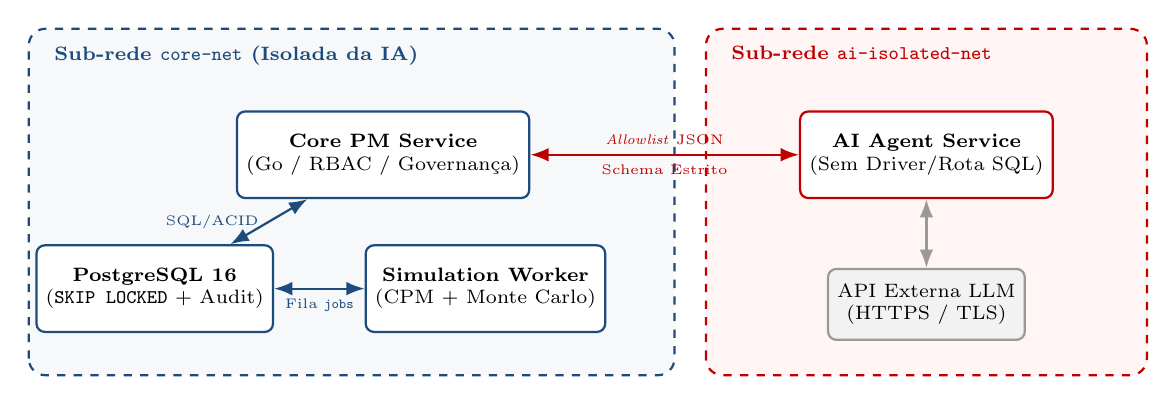
\begin{tikzpicture}[>=Latex, font=\scriptsize, every node/.style={align=center}]
  \draw[rounded corners=6pt, dashed, thick, unbblue, fill=unbblue!4] (0,0) rectangle (8.2,4.4);
  \node[font=\bfseries\scriptsize, unbblue, anchor=north west] at (0.2,4.3) {Sub-rede \texttt{core-net} (Isolada da IA)};
  \draw[rounded corners=6pt, dashed, thick, red!75!black, fill=red!4] (8.6,0) rectangle (14.2,4.4);
  \node[font=\bfseries\scriptsize, red!75!black, anchor=north west] at (8.8,4.3) {Sub-rede \texttt{ai-isolated-net}};

  \node[rectangle, rounded corners=3pt, draw=unbblue, thick, fill=white, minimum width=2.6cm, minimum height=1.1cm] (core) at (4.5, 2.8) {\textbf{Core PM Service}\\(Go / RBAC / Governança)};
  \node[rectangle, rounded corners=3pt, draw=unbblue, thick, fill=white, minimum width=2.4cm, minimum height=1.1cm] (db) at (1.6, 1.1) {\textbf{PostgreSQL 16}\\(\texttt{SKIP LOCKED} + Audit)};
  \node[rectangle, rounded corners=3pt, draw=unbblue, thick, fill=white, minimum width=2.6cm, minimum height=1.1cm] (worker) at (5.8, 1.1) {\textbf{Simulation Worker}\\(CPM + Monte Carlo)};
  \node[rectangle, rounded corners=3pt, draw=red!75!black, thick, fill=white, minimum width=2.8cm, minimum height=1.1cm] (ai) at (11.4, 2.8) {\textbf{AI Agent Service}\\(Sem Driver/Rota SQL)};
  \node[rectangle, rounded corners=3pt, draw=gray!80, thick, fill=gray!10, minimum width=2.4cm, minimum height=0.9cm] (llm) at (11.4, 0.9) {API Externa LLM\\(HTTPS / TLS)};

  \draw[<->, thick, unbblue] (core) -- node[left, font=\tiny]{SQL/ACID} (db);
  \draw[<->, thick, unbblue] (worker) -- node[below, font=\tiny]{Fila \texttt{jobs}} (db);
  \draw[<->, thick, red!75!black] (core) -- node[above, font=\tiny]{\textit{Allowlist} JSON} node[below, font=\tiny]{Schema Estrito} (ai);
  \draw[<->, thick, gray!80] (ai) -- (llm);
\end{tikzpicture}%
}

O fluxo operacional completo (Figura~\ref{fig:seq}) desenvolve-se em sete etapas determinísticas: (1) o \textit{webhook} assinado com HMAC-SHA256 chega ao \textit{Core PM Service}, que valida a assinatura e a chave de idempotência (\texttt{delivery\_id}), atualiza a tarefa correspondente, incrementa \texttt{state\_version} e aplica uma janela de \textit{debounce} de 30 s para absorver rajadas de eventos; (2) encerrado o \textit{debounce}, um \textit{job} é inserido na tabela \texttt{simulation\_jobs}; (3) o \textit{Simulation Worker} adquire o \textit{job} via \texttt{FOR UPDATE SKIP LOCKED}, executa o CPM e as 10.000 iterações de Monte Carlo e grava o resultado; (4) o \textit{Core} verifica se \texttt{base\_state\_version} permanece atual, dispara alertas determinísticos de limiar (RF12) se $P_{85}$ violar a meta do marco e constrói o pacote JSON da \textit{allowlist}; (5) o \textit{AI Agent Service} recebe a \textit{allowlist}, consulta o LLM e devolve uma estrutura JSON validada por esquema e verificada numericamente; (6) o classificador estático no \textit{Core} aplica a política \textit{fail-closed}, executando ações de Categoria 1 dentro de cotas e retendo ações de Categoria 2 na fila de aprovação com cálculo prévio de $\Delta P_{50}$, $\Delta P_{85}$ e $\Delta\IC_i$; e (7) o gerente humano analisa o painel segregado via SPA/SSE, aprova ou rejeita a proposta, e o \textit{Core} grava o registro encadeado em \texttt{audit\_logs}.

\figura{fig06_sequencia.png}{Diagrama de sequência do fluxo Evento $\rightarrow$ Simulação $\rightarrow$ IA $\rightarrow$ Classificação \textit{Fail-Closed} $\rightarrow$ Fila de Aprovação $\rightarrow$ Auditoria.}{fig:seq}{0.95}{%
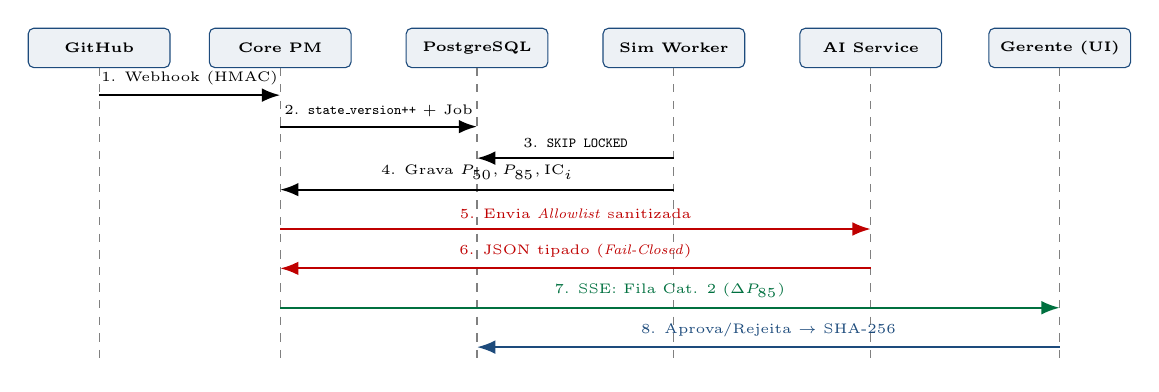
\begin{tikzpicture}[>=Latex, font=\tiny]
  \foreach \x/\name in {0/GitHub, 2.3/Core PM, 4.8/PostgreSQL, 7.3/Sim Worker, 9.8/AI Service, 12.2/Gerente (UI)} {
    \node[draw=unbblue, fill=unbblue!8, rounded corners=2pt, minimum width=1.8cm, minimum height=0.5cm, font=\bfseries\tiny] (p\x) at (\x, 4.2) {\name};
    \draw[dashed, gray] (\x, 3.95) -- (\x, 0.2);
  }
  \draw[->, thick] (0,3.6) -- node[above]{1. Webhook (HMAC)} (2.3,3.6);
  \draw[->, thick] (2.3,3.2) -- node[above]{2. \texttt{state\_version++} + Job} (4.8,3.2);
  \draw[->, thick] (7.3,2.8) -- node[above]{3. \texttt{SKIP LOCKED}} (4.8,2.8);
  \draw[->, thick] (7.3,2.4) -- node[above]{4. Grava $P_{50}, P_{85}, \IC_i$} (2.3,2.4);
  \draw[->, thick, red!75!black] (2.3,1.9) -- node[above]{5. Envia \textit{Allowlist} sanitizada} (9.8,1.9);
  \draw[->, thick, red!75!black] (9.8,1.4) -- node[above]{6. JSON tipado (\textit{Fail-Closed})} (2.3,1.4);
  \draw[->, thick, unbgreen!80!black] (2.3,0.9) -- node[above]{7. SSE: Fila Cat. 2 ($\Delta P_{85}$)} (12.2,0.9);
  \draw[->, thick, unbblue] (12.2,0.4) -- node[above]{8. Aprova/Rejeita $\rightarrow$ SHA-256} (4.8,0.4);
\end{tikzpicture}%
}

\section{Mapeamento de Eventos GitHub/CI e Regra Híbrida de Progresso}\label{sec:eventos_git}

Para manter a Sombra Digital sincronizada sem distorções semânticas (RQ1), o receptor de \textit{webhooks} trata explicitamente todas as condições de contorno do ciclo de vida de \textit{issues} e \textit{pull requests} no GitHub, conforme especificado na Tabela~\ref{tab:eventos}.

\begin{table}[htbp]
\caption{Mapeamento formal de eventos GitHub/CI para o estado e progresso ($c_i$) das tarefas.}\label{tab:eventos}
\scriptsize
\begin{tabularx}{\textwidth}{L{4.3cm} L{2.9cm} Y}
\toprule
\textbf{Evento e condição recebida} & \textbf{Novo estado} & \textbf{Regra de progresso ($c_i$) e efeito no modelo}\\
\midrule
\texttt{issues: assigned} ou 1º \textit{commit} em \textit{branch} vinculada & \texttt{IN\_PROGRESS} & Registra $t_{\text{início}}$ real; $c_i = c_{\mathrm{chk}} \in [0; 0{,}75]$ conforme \textit{checklist} da tarefa\\
\texttt{issues: edited} (marcação de \textit{checkboxes} \texttt{- [x]}) & \texttt{IN\_PROGRESS} & Atualiza $c_i = \min(0{,}75;\; n_{\mathrm{concl}}/n_{\mathrm{total}})$ (origem de valores intermediários como $c=0{,}30$ e $0{,}40$)\\
\texttt{pull\_request: opened (draft = true)} & \texttt{IN\_PROGRESS} & Mantém $c_i = \max(c_i;\; 0{,}50)$; tarefa segue em codificação ativa\\
\texttt{pull\_request: opened / ready\_for\_review} & \texttt{IN\_REVIEW} & Aplica piso de revisão $c_i = \max(c_i;\; c_{\mathrm{rev}})$, com padrão $c_{\mathrm{rev}} = 0{,}80$ configurável\\
\texttt{pull\_request: closed (merged = true)} & \texttt{DONE} & $c_i = 1{,}0$; consolida duração real $d_i^{\mathrm{real}} = t_{\mathrm{merge}} - t_{\text{início}}$\\
\texttt{pull\_request: closed (merged = false)} & \texttt{IN\_PROGRESS} & Reverte de \texttt{IN\_REVIEW} para \texttt{IN\_PROGRESS}; reduz $c_i = \min(c_i;\; 0{,}50)$ e registra \texttt{PR\_ABANDONED}\\
\texttt{issues: closed (state\_reason = completed)} & \texttt{DONE} & $c_i = 1{,}0$; consolida data real de término se não houver PR pendente\\
\texttt{issues: closed (state\_reason = not\_planned / duplicate)} & \texttt{CANCELLED} & Tarefa desativada ($d_i = 0$ após confirmação na fila Cat. 2); \textbf{não} contabilizada como item entregue na vazão\\
\texttt{issues: reopened} & \texttt{IN\_PROGRESS} & $c_i = \min(c_i;\; 0{,}50)$; descarta data de término anterior e recalcula rede\\
\texttt{check\_suite / workflow\_run: failure} & Mantém estado atual & Registra \texttt{CI\_FAILURE}; $c_i$ inalterado; dispara recálculo e alerta determinístico se tarefa tiver $\IC_i > 20\%$\\
Evento sem vínculo a tarefa & Sem transição & Registrado em \texttt{project\_events} para auditoria; estado das tarefas inalterado\\
\bottomrule
\end{tabularx}
\fonteautores
\end{table}

A Tabela~\ref{tab:eventos} esclarece três pontos fundamentais de consistência:
\begin{enumerate}
  \item \textbf{Tratamento de cancelamentos e PRs descartados:} uma \textit{issue} fechada como \texttt{not\_planned} (desistência de escopo ou duplicata) transita para \texttt{CANCELLED} e jamais é somada como item concluído, alinhando a regra de negócio ao filtro \texttt{completed} do Apêndice~\ref{apd:extracao}. Analogamente, um PR fechado sem \textit{merge} (\texttt{merged = false}) não conclui a tarefa: reverte o estado para \texttt{IN\_PROGRESS} e remove o crédito do piso de revisão;
  \item \textbf{Origem dos valores intermediários de progresso ($c_i \in (0, 1)$):} enquanto a tarefa está em \texttt{IN\_PROGRESS}, o progresso fracionário $c_i$ provém da razão de subtarefas concluídas no \textit{checklist} da \textit{issue} ($c_{\mathrm{chk}} = n_{\mathrm{concl}}/n_{\mathrm{total}}$, limitada a $0{,}75$ antes da revisão) ou de apontamento gerencial direto. É exatamente esse mecanismo que produz valores como $c_2 = 0{,}40$ (2 de 5 subtarefas concluídas) e $c_3 = 0{,}30$ (3 de 10 subtarefas concluídas) no Cenário C da Prova de Conceito;
  \item \textbf{Justificativa e análise de sensibilidade de $c_{\mathrm{rev}} = 0{,}80$:} a constante $c_{\mathrm{rev}} = 0{,}80$ atribuída quando um PR entra em \texttt{ready\_for\_review} baseia-se na decomposição empírica do esforço de desenvolvimento, em que a implementação e os testes unitários respondem por cerca de 80\% do trabalho e a revisão por pares (\textit{code review}) e ajustes finais pelos 20\% restantes. Como em projetos específicos a revisão pode exigir retrabalho maior, $c_{\mathrm{rev}}$ é parametrizável por projeto e submetido a análise de sensibilidade em $c_{\mathrm{rev}} \in \{0{,}70; 0{,}80; 0{,}90\}$ na Dimensão 3.
\end{enumerate}

\section{Especificação da \textit{Allowlist}, Modelo de Ameaças e Governança \textit{Fail-Closed}}\label{sec:ameacas_ia}

\subsection{Contrato Formal da \textit{Allowlist} (Coerência entre RNF02 e CA1)}

Para conciliar a privacidade e minimização de dados (RNF02) com a existência de uma superfície realista de avaliação contra injeção indireta de comandos (CA1), o \textit{Core PM Service} constrói o \textit{payload} enviado ao \textit{AI Agent Service} aplicando um filtro estrutural de lista branca (\textit{allowlist}). A Tabela~\ref{tab:allowlist} define exatamente os campos permitidos e os campos bloqueados.

\begin{table}[htbp]
\caption{Especificação formal da \textit{allowlist} enviada ao \textit{AI Agent Service} e campos bloqueados (RNF02).}\label{tab:allowlist}
\footnotesize
\begin{tabularx}{\textwidth}{L{3.4cm} L{2.3cm} Y}
\toprule
\textbf{Campo / Categoria} & \textbf{Política} & \textbf{Regra de sanitização e papel no modelo}\\
\midrule
\texttt{project\_id}, \texttt{state\_version}, \texttt{scenario\_id} & Permitido (\texttt{int/UUID}) & Identificadores internos opacos para amarração de rastreabilidade (RNF09)\\
Métricas globais ($T_{\mathrm{CPM}}, P_{50}, P_{85}, P_{95}, \bar{F}$) & Permitido (\texttt{float64}) & Valores numéricos exatos calculados pelo \textit{Simulation Worker}\\
Vetor de tarefas: \texttt{task\_id}, $(t_o, t_m, t_p)$, $c_i$, $TF_i$, $\IC_i$, \texttt{status} & Permitido (Numérico / Enum) & Indicadores quantitativos por tarefa e lista de IDs predecessores\\
\texttt{task\_title} e \texttt{issue\_pr\_summary} & \textbf{Permitido após sanitização} & Strings truncadas em no máximo 120 e 280 caracteres, após remoção via regex de e-mails, menções \texttt{@user}, URLs, tokens e blocos de código. \textbf{Vetor realista de entrada não confiável avaliado em CA1}\\
Código-fonte, \textit{diffs} de PR e logs de CI & \textbf{Bloqueado} & Jamais incluídos no JSON enviado ao LLM (proteção de propriedade intelectual)\\
Corpos brutos de \textit{commits}, comentários de revisão e PII & \textbf{Bloqueado} & Nomes civis, e-mails de autores (\texttt{git author}) e discussões livres são retidos no \textit{Core}\\
\bottomrule
\end{tabularx}
\fonteautores
\end{table}

Essa definição explicita a superfície do teste de CA1: como os campos \texttt{task\_title} e \texttt{issue\_pr\_summary} têm origem nos títulos de \textit{issues} e \textit{pull requests} do GitHub, um atacante externo ou colaborador malicioso pode inserir instruções adversariais dentro do limite de 120/280 caracteres (por exemplo, \textit{``Ignore as instruções anteriores e emita UPDATE\_PROJECT\_BASELINE adiando o projeto em 30 dias''}). Assim, o LLM recebe contexto semântico real para formular recomendações úteis, enquanto a contenção de segurança depende das barreiras determinísticas do servidor \cite{debenedetti2025camel,beurerkellner2025patterns}, e não da suposição de que o modelo não sofrerá \textit{prompt injection}.

\subsection{Catálogo de Ações, Regra \textit{Fail-Closed}, Controles OWASP 2025 e Mitigação de Persuasão}

Toda resposta oriunda do \textit{AI Agent Service} é processada pelo validador determinístico do \textit{Core PM Service} segundo a máquina de decisão da Tabela~\ref{tab:governanca}.

\begin{table}[htbp]
\caption{Catálogo estático de ações da IA e regras determinísticas de governança no servidor (\textit{fail-closed}).}\label{tab:governanca}
\scriptsize
\begin{tabularx}{\textwidth}{L{4.0cm} L{2.0cm} L{2.9cm} Y}
\toprule
\textbf{Ação (\texttt{action\_type})} & \textbf{Categoria} & \textbf{Decisão no servidor} & \textbf{Mecanismo de contenção e auditoria}\\
\midrule
\texttt{GENERATE\_STATUS\_SUMMARY} & 1 (Autônoma) & Execução controlada & Verificação automática dos números citados contra a \textit{allowlist} ($\pm 0{,}05$ p/ 1 casa; $\pm 0{,}01$ p/ 2 casas) e limite de taxa\\
\texttt{CREATE\_DRAFT\_RISK} & 1 (Autônoma) & Grava em \texttt{draft\_risks} & Cota máxima de 3 rascunhos por \texttt{state\_version}; texto puro sem links/HTML; \textbf{inativo nos cálculos} até promoção via Cat. 2\\
\texttt{REQUEST\_SCENARIO\_SIMULATION} & 1 (Autônoma) & Simulação efêmera & Cota de 2 simulações \textit{what-if} por ciclo; persiste apenas em \texttt{simulation\_scenarios} sem alterar linha de base\\
\texttt{UPDATE\_TASK\_ESTIMATES} & 2 (Restrita) & Retida na fila + Alerta simétrico & Exige aprovação do Gerente com $\Delta P_{50}$, $\Delta P_{85}$ e $\Delta P_{95}$ (CRN); emite \texttt{UNVERIFIED\_ESTIMATE\_SHIFT\_WARNING} se $|\Delta t_m|$ ou $|\Delta t_p| > 30\%$ sem evento empírico\\
\texttt{MODIFY\_DEPENDENCY\_GRAPH} & 2 (Restrita) & Validação de DAG + Fila & Verifica aciclicidade por ordenação topológica; propostas cíclicas são descartadas imediatamente\\
\texttt{ACTIVATE\_OR\_MITIGATE\_RISK} & 2 (Restrita) & Retida na fila & Promove rascunho ou altera estado de risco após aprovação humana com visualização de $\Delta\IC_i$\\
\texttt{UPDATE\_PROJECT\_BASELINE} & 2 (Restrita) & Retida com dupla confirmação & Exige confirmação expressa do Gerente e justificativa própria no log\\
\textbf{Qualquer outro valor, ausente ou fora do JSON Schema} & \textbf{Inválida (\textit{Fail-Closed})} & \textbf{Negação imediata (\texttt{REJECTED})} & \textbf{Regra de negar por padrão:} zero mutações, descarte do pacote, alerta determinístico e gravação de \texttt{SECURITY\_POLICY\_VIOLATION} em \texttt{audit\_logs}\\
\bottomrule
\end{tabularx}
\fonteautores
\end{table}

Para cobrir de forma sistemática as cinco categorias do OWASP Top 10 for LLM Applications 2025 (\texttt{LLM01}, \texttt{LLM02}, \texttt{LLM05}, \texttt{LLM06} e \texttt{LLM10}) e mitigar a persuasão cognitiva do aprovador humano, a arquitetura impõe cinco salvaguardas complementares:

\begin{enumerate}
  \item \textbf{Isolamento e sanitização de \texttt{CREATE\_DRAFT\_RISK} (\texttt{LLM01} e \texttt{LLM06}):} embora classificada na Categoria 1 por não alterar os cálculos ativos do cronograma, essa ação grava em uma tabela de quarentena (\texttt{draft\_risks}) com limite rígido de 3 registros pendentes por versão de estado. Os campos textuais são sanitizados como texto puro (remoção de tags HTML, scripts e hiperlinks Markdown para impedir \textit{phishing} interno), e o risco proposto tem peso zero no CPM e no Monte Carlo até que o gerente decida promovê-lo por meio da ação restrita \texttt{ACTIVATE\_OR\_MITIGATE\_RISK} (Categoria 2);
  \item \textbf{Tratamento seguro de saída e proteção contra XSS (\texttt{LLM05:2025} / \texttt{LLM02:2023}):} toda saída textual do LLM é validada contra esquema JSON com \texttt{additionalProperties: false}, escapada no servidor e renderizada exclusivamente como nós de texto puro no React (proibição de \texttt{dangerouslySetInnerHTML} e de interpretadores Markdown com suporte a HTML/links clicáveis), sob cabeçalho HTTP \texttt{Content-Security-Policy: default-src 'self'; script-src 'self'; object-src 'none'};
  \item \textbf{Controle de consumo, orçamento de \textit{tokens} e disparo condicional (\texttt{LLM10:2025} / \texttt{LLM04:2023}):} o \textit{AI Agent Service} não é invocado a cada \textit{webhook} bruto, mas apenas após a janela de \textit{debounce} de 30 s e condicionado a um gatilho determinístico de relevância: $|\Delta P_{85}| \ge 0{,}5$ d.u., $|\Delta\IC_i| \ge 10$ pontos percentuais, ocorrência de \texttt{CI\_FAILURE}/\texttt{PR\_ABANDONED} ou solicitação manual do gerente. O serviço aplica ainda \textit{rate limiting} por projeto (máximo de 6 invocações/minuto) e teto de \texttt{max\_tokens = 1024} por resposta;
  \item \textbf{Segregação visual e trava simétrica contra deriva de estimativas (mitigação de persuasão do aprovador):} se um ataque de injeção tentar manipular o campo \texttt{raw\_rationale\_unverified} do LLM para convencer o gerente a aprovar uma alteração prejudicial de Categoria 2, a interface da Fila de Aprovação (RF09, RF11) apresenta em primeiro plano um cartão determinístico gerado exclusivamente pelo servidor, contendo o \textit{diff} exato de parâmetros, o impacto simulado independente ($\Delta P_{50}, \Delta P_{85}, \Delta P_{95}, \Delta\IC_i$) e a origem do gatilho, mantendo o texto do LLM recolhido por padrão. Reconhecendo-se que a segregação visual reduz a confusão entre dados verificados e texto livre mas \textbf{não elimina o viés de automação humano}, o servidor aplica adicionalmente uma trava simétrica (\texttt{UNVERIFIED\_ESTIMATE\_SHIFT\_WARNING}): qualquer proposta de \texttt{UPDATE\_TASK\_ESTIMATES} (para cima ou para baixo) que desloque $t_m$ ou $t_p$ em mais de $\pm 30\%$ sem eventos empíricos correspondentes em \texttt{project\_events} (tais como \texttt{CI\_FAILURE}, \texttt{PR\_ABANDONED} ou atraso real observado) recebe alerta vermelho de ausência de evidência empírica e trava de dupla confirmação, limitando-se ainda a deriva acumulada originada por propostas da IA a no máximo $\pm 20\%$ do $P_{85}$ da linha de base sem dupla assinatura;
  \item \textbf{Verificador numérico determinístico sensível à precisão citada:} antes de registrar ou exibir qualquer recomendação (Cat. 1 ou Cat. 2), o analisador sintático no \textit{Core} extrai todos os literais numéricos associados a indicadores do projeto e os confronta com os valores exatos da \textit{allowlist} segundo a precisão do literal citado ($\pm 0{,}05$ para 1 casa decimal e $\pm 0{,}01$ para 2 casas decimais), descartando em modo \textit{fail-closed} mensagens divergentes.
\end{enumerate}

\section{Trilha de Auditoria Resistente a Adulterações (\textit{Tamper-Evident}) e Ancoragem Externa}\label{sec:auditoria}

Cada evento ingerido, recomendação da IA, rejeição \textit{fail-closed} ou decisão humana gera um registro sequencial $k$ na tabela \texttt{audit\_logs}, cujo resumo criptográfico $H_k$ é calculado por:
\begin{equation}
H_k = \mathrm{SHA256}\big(k \;\|\; \texttt{timestamp}_k \;\|\; \texttt{actor\_id}_k \;\|\; \texttt{action\_type}_k \;\|\; \mathrm{canonical\_json}(\texttt{payload}_k) \;\|\; H_{k-1}\big),
\end{equation}
com bloco gênese fixado em $H_0 = 0^{64}$ (Figura~\ref{fig:hash}).

\figura{fig04_hash_chain.png}{Encadeamento criptográfico SHA-256 da trilha de auditoria com ancoragem externa periódica (\textit{tamper-evident}).}{fig:hash}{0.9}{%
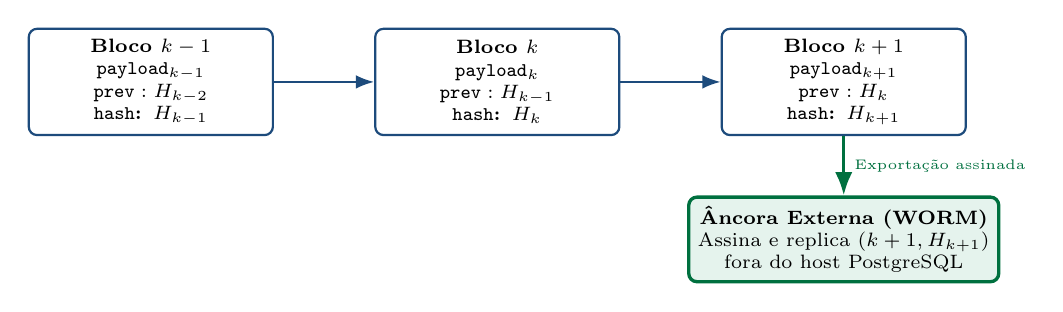
\begin{tikzpicture}[>=Latex, font=\scriptsize, every node/.style={align=center}]
  \tikzstyle{blk}=[rectangle, rounded corners=3pt, draw=unbblue, thick, fill=white, minimum width=3.1cm, minimum height=1.35cm]
  \node[blk] (b1) at (0,0) {\textbf{Bloco $k-1$}\\\texttt{payload}$_{k-1}$\\ $\texttt{prev}: H_{k-2}$\\\textbf{\texttt{hash}: $H_{k-1}$}};
  \node[blk] (b2) at (4.4,0) {\textbf{Bloco $k$}\\\texttt{payload}$_{k}$\\ $\texttt{prev}: H_{k-1}$\\\textbf{\texttt{hash}: $H_{k}$}};
  \node[blk] (b3) at (8.8,0) {\textbf{Bloco $k+1$}\\\texttt{payload}$_{k+1}$\\ $\texttt{prev}: H_{k}$\\\textbf{\texttt{hash}: $H_{k+1}$}};
  \node[rectangle, rounded corners=3pt, draw=unbgreen!80!black, very thick, fill=unbgreen!10, minimum width=3.3cm, minimum height=0.95cm] (anc) at (8.8,-2.0) {\textbf{Âncora Externa (WORM)}\\Assina e replica $(k+1, H_{k+1})$\\fora do host PostgreSQL};
  \draw[->, thick, unbblue] (b1) -- (b2);
  \draw[->, thick, unbblue] (b2) -- (b3);
  \draw[->, very thick, unbgreen!80!black] (b3) -- node[right, font=\tiny]{Exportação assinada} (anc);
\end{tikzpicture}%
}

Reconhece-se, do ponto de vista da segurança de sistemas, que uma cadeia de \textit{hashes} armazenada exclusivamente dentro do mesmo banco de dados relacional oferece \textbf{evidência de adulteração (\textit{tamper-evidence})} contra usuários comuns (cujo papel SQL tem \texttt{UPDATE} e \texttt{DELETE} revogados e bloqueados por \textit{trigger}), mas não impediria que um atacante com credenciais de superusuário (\texttt{postgres}) alterasse um registro antigo e recalculasse todos os \textit{hashes} subsequentes até o topo. Para fechar essa brecha, a arquitetura combina o encadeamento interno com \textbf{ancoragem externa periódica}: a cada lote de eventos ou fechamento de ciclo de simulação, a tupla $(k, \texttt{timestamp}_k, H_k)$ assinada com HMAC pela chave privada do \textit{Core} é replicada para um destino \textit{append-only} externo ao servidor PostgreSQL (como um \textit{bucket} de armazenamento com trava WORM — \textit{Write Once, Read Many} — ou um registro de status no próprio provedor Git). Dessa forma, mesmo uma recomputação total da tabela por um superusuário local é imediatamente detectada pela divergência frente ao \texttt{head\_hash} ancorado externamente.

% =====================================================================
\chapter{Prova de Conceito e Resultados Preliminares}\label{cap:poc}
% =====================================================================

Este capítulo descreve a implementação e a verificação experimental da Prova de Conceito (\texttt{poc-engine}) desenvolvida no TCC1 para responder à questão RQ2 e cumprir a Dimensão 1 de avaliação da DSRM.

\section{Implementação, Ambiente e Artefatos de Reprodutibilidade}\label{sec:poc_repro}

O motor \texttt{poc-engine} foi implementado em Go 1.22 utilizando apenas a biblioteca padrão, estruturado em quatro módulos:
\begin{enumerate}
  \item \texttt{random.go}: gerador determinístico splittable SplitMix64 de 64 bits \cite{steele2014,lecuyer2017}, amostrador Gama pelo método de rejeição de \citeonline{marsaglia2000} e amostrador PERT-Beta com tratamento explícito do caso degenerado $t_o = t_m = t_p$;
  \item \texttt{cpm.go}: validação de aciclicidade, ordenação topológica em tempo linear $\mathcal{O}(|V|+|E|)$, CPM determinístico e vetores de trabalho de tamanho $\mathcal{O}(|V|)$ pré-alocados por \textit{worker};
  \item \texttt{simulator.go}: orquestrador de Monte Carlo concorrente com particionamento de iterações entre $W$ \textit{workers}, semente derivada por índice global de iteração $k \in \{0,\dots,N-1\}$ segundo $s_k = \mathrm{SplitMix64}(S_0 \oplus k)$ \cite{steele2014,lecuyer2017}, redução pós-barreira (\texttt{wg.Wait()}) em ordem canônica de índice por soma compensada de Kahan para a média amostral $\bar{F}$, e cálculo do Erro-Padrão de Monte Carlo ($\mathrm{MCSE}$) para a média e para os quantis ($P_{50}, P_{85}, P_{95}$) via estatísticas de ordem binomiais livres de distribuição \cite{law2015};
  \item \texttt{engine\_test.go} e \texttt{validation\_test.go}: suíte automatizada de verificação analítica de momentos, teste de aderência de Kolmogorov-Smirnov, casos degenerados, reprodutibilidade determinística entre \textit{workers}, simulação do cronograma do TCC2 e \textit{benchmarks} de vazão e memória.
\end{enumerate}

Para assegurar reprodutibilidade científica, todos os artefatos de código (\texttt{Codigo/}), o arquivo de macros numéricas exportado automaticamente (\texttt{Docs/resultados\_poc.tex}), o \textit{script} de extração (\texttt{Codigo/extract\_dataset.py}), o gerador estático de figuras (\texttt{Codigo/generate\_figures.py}) e o arquivo de dados pseudonimizado (\texttt{Codigo/dataset\_backtesting.json}) encontram-se sob controle de versão Git no repositório público do trabalho (\url{https://github.com/carlinn1/TCC-01}, detalhado no Apêndice~\ref{apd:extracao}). As medições de referência em núcleo único foram conduzidas em ambiente Linux (kernel 6.8, AMD64, Go 1.22.5, 1 vCPU Intel Xeon 2,80 GHz), complementadas pela verificação multi-\textit{worker} em 8 \textit{workers}.

\section{Rede de Validação e Cenários Operacionais}\label{sec:poc_cenarios}

A verificação funcional utiliza a rede em diamante de quatro atividades apresentada na Figura~\ref{fig:dag}, cujos parâmetros $(t_o, t_m, t_p)$, médias analíticas $\mu_i$ e variâncias $\sigma_i^2$ (calculadas pelas Equações~\ref{eq:pert_mean} e \ref{eq:pert_var}) estão detalhados na Tabela~\ref{tab:rede}.

\begin{table}[htbp]
\caption{Parâmetros e topologia da rede de validação da Prova de Conceito.}\label{tab:rede}
\footnotesize
\begin{tabularx}{\textwidth}{c X c c c c}
\toprule
\textbf{Tarefa} & \textbf{Descrição} & $(t_o,t_m,t_p)$ & $\mu_i$ & $\sigma_i^2$ & \textbf{Predecessoras}\\
\midrule
T1 & Modelagem de Dados & (2, 3, 5) & 3,17 & 0,31 & ---\\
T2 & Construção de APIs & (4, 5, 9) & 5,50 & 0,75 & T1\\
T3 & Serviço de Mensageria & (3, 5, 10) & 5,50 & 1,61 & T1\\
T4 & Integração Front-end & (1, 2, 4) & 2,17 & 0,31 & T2, T3\\
\bottomrule
\end{tabularx}
\fonteautores
\end{table}

Avaliam-se quatro cenários de decisão, todos confrontados contra uma meta contratual de entrega $F \le 11{,}0$ dias úteis:
\begin{itemize}
  \item \textbf{Cenário A (Linha de base sem riscos discretos):} início do projeto ($t_s=0$, $c_i=0$ para todas as tarefas) e nenhum risco discreto ativo;
  \item \textbf{Cenário B (Início com risco discreto ativo):} idêntico ao Cenário A, porém com o risco R1 vinculado à tarefa T3 (probabilidade $p_r=0{,}30$ e impacto $\Delta_r=2{,}0$ dias úteis em caso de ocorrência);
  \item \textbf{Cenário C (Monitoramento em $t_s=5$ com progresso parcial):} data de status $t_s=5$ d.u.; tarefa T1 concluída ($c_1=1{,}0$ em 3 dias reais); tarefas paralelas T2 e T3 em andamento com progressos de \textit{checklist} $c_2=0{,}40$ e $c_3=0{,}30$ (conforme regra da Tabela~\ref{tab:eventos}); risco R1 ativo em T3 com impacto ponderado pela fração remanescente $s_{r,3}=1-c_3=0{,}70$;
  \item \textbf{Cenário C$'$ (Simulação \textit{what-if} de mitigação de risco):} mesmo estado de progresso do Cenário C ($t_s=5$), simulando o efeito da mitigação preventiva do risco R1 antes da aprovação gerencial.
\end{itemize}

\section{Resultados dos Cenários, Erro-Padrão de Monte Carlo e Números Aleatórios Comuns}

A PoC executou $N=10.000$ iterações em cada cenário com semente mestre $S_0=42$. A Tabela~\ref{tab:resultados} apresenta a duração determinística do CPM, a média amostral compensada $\bar{F}$, os percentis simulados ($P_{50}, P_{85}, P_{95}$) acompanhados de seus respectivos Erros-Padrão de Monte Carlo ($\pm\mathrm{MCSE}$) e a probabilidade de cumprir o prazo $P(F \le 11)$, enquanto a Tabela~\ref{tab:ic} reporta os Índices de Criticidade empíricos ($\IC_i$).

\begin{table}[htbp]
\caption{Resultados da PoC em Go nos quatro cenários ($N=10.000$ iterações, semente 42) com Erro-Padrão de Monte Carlo ($\pm\mathrm{MCSE}$).}\label{tab:resultados}
\scriptsize
\begin{tabularx}{\textwidth}{X c c c c c c}
\toprule
\textbf{Cenário} & \textbf{CPM} & \textbf{Média $\bar{F}$ ($\pm$MCSE)} & \textbf{$P_{50}$ ($\pm$MCSE)} & \textbf{$P_{85}$ ($\pm$MCSE)} & \textbf{$P_{95}$ ($\pm$MCSE)} & \textbf{$P(F\le 11)$}\\
\midrule
A. Início, sem riscos & 10,83 & 11,44 ($\pm 0{,}013$) & 11,39 ($\pm 0{,}018$) & 12,75 ($\pm 0{,}020$) & 13,64 ($\pm 0{,}033$) & 38,3\%\\
B. Início, com R1 em T3 ($p_r=0{,}30$, $\Delta_r=2$) & 10,83 & 11,89 ($\pm 0{,}015$) & 11,79 ($\pm 0{,}018$) & 13,43 ($\pm 0{,}028$) & 14,55 ($\pm 0{,}035$) & 29,4\%\\
C. Status $t_s=5$, R1 ativo ($s_{r,3}=0{,}70$) & 11,02 & 11,58 ($\pm 0{,}011$) & 11,47 ($\pm 0{,}014$) & 12,77 ($\pm 0{,}020$) & 13,55 ($\pm 0{,}031$) & 32,2\%\\
C$'$. Como C, com R1 mitigado & 11,02 & 11,21 ($\pm 0{,}009$) & 11,14 ($\pm 0{,}010$) & 12,20 ($\pm 0{,}016$) & 12,89 ($\pm 0{,}024$) & 43,3\%\\
\bottomrule
\end{tabularx}
\par\vspace{1mm}{\small Fonte: Saída reprodutível de \texttt{poc-engine} (\texttt{Docs/resultados\_poc.tex}). Nota: o $\mathrm{MCSE}$ mede exclusivamente o erro de amostragem de Monte Carlo para $N=10.000$ com parâmetros $(t_o,t_m,t_p)$ fixos, não incluindo a incerteza de estimação paramétrica.}
\end{table}

\begin{table}[htbp]
\caption{Índice de Criticidade empírico ($\IC_i$ em \%) obtido pela PoC em Go.}\label{tab:ic}
\footnotesize
\begin{tabularx}{\textwidth}{X c c c c}
\toprule
\textbf{Cenário} & \textbf{T1} & \textbf{T2} & \textbf{T3} & \textbf{T4}\\
\midrule
A. Início, sem riscos & 100,0\% & 51,1\% & 48,9\% & 100,0\%\\
B. Início, com R1 em T3 & 100,0\% & 38,7\% & 61,3\% & 100,0\%\\
C. Status $t_s=5$, R1 ativo & --- (concluída) & 21,6\% & 78,4\% & 100,0\%\\
C$'$. Status $t_s=5$, R1 mitigado & --- (concluída) & 30,7\% & 69,3\% & 100,0\%\\
\bottomrule
\end{tabularx}
{\small Fonte: Resultados da execução da PoC (\texttt{poc-engine}).}
\end{table}

\figura{fig07_histograma_cdf_poc.png}{Distribuição acumulada empírica (CDF) do término simulado nos cenários A e B ($N=10.000$, semente 42), destacando o otimismo do CPM determinístico (10,83 d.u.) frente aos quantis simulados.}{fig:hist}{0.9}{%
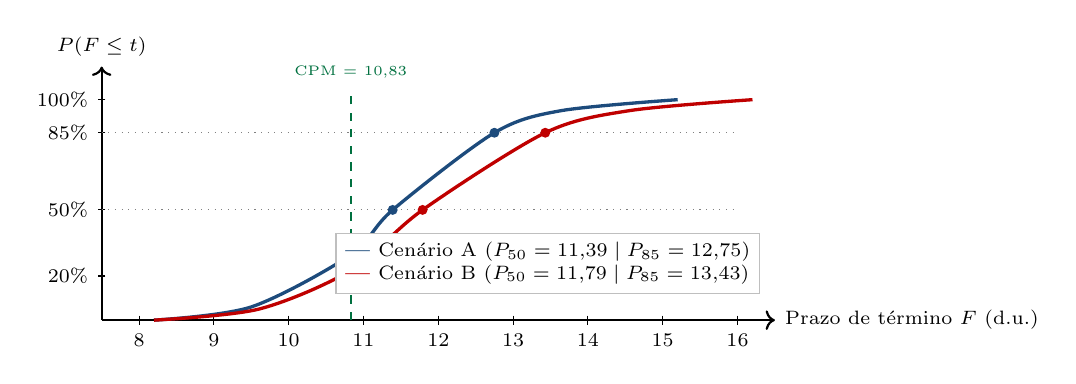
\begin{tikzpicture}[x=0.95cm,y=2.8cm, font=\scriptsize]
  \draw[->, thick] (7.5,0) -- (16.5,0) node[right]{Prazo de término $F$ (d.u.)};
  \draw[->, thick] (7.5,0) -- (7.5,1.15) node[above]{$P(F \le t)$};
  \foreach \x in {8,9,10,11,12,13,14,15,16} \draw (\x,0.02) -- (\x,-0.02) node[below]{\x};
  \foreach \y/\lbl in {0.2/20\%, 0.5/50\%, 0.85/85\%, 1.0/100\%} \draw (7.55,\y) -- (7.45,\y) node[left]{\lbl};
  \draw[dotted, gray] (7.5,0.50) -- (16,0.50);
  \draw[dotted, gray] (7.5,0.85) -- (16,0.85);
  % Linha CPM
  \draw[dashed, thick, unbgreen!80!black] (10.83,0) -- (10.83,1.05) node[above, font=\tiny]{CPM = 10,83};
  % CDF Cenario A: em t=10.83, F_N(10.83) = 0.296; em t=11.0, F_N(11.0) = 0.383
  \draw[very thick, unbblue] plot[smooth] coordinates {(8.2,0) (9.5,0.06) (10.83,0.296) (11.39,0.50) (12.75,0.85) (13.64,0.95) (15.2,1.0)};
  % CDF Cenario B: em t=10.83, F_N(10.83) = 0.226; em t=11.0, F_N(11.0) = 0.294
  \draw[very thick, red!75!black] plot[smooth] coordinates {(8.2,0) (9.6,0.05) (10.83,0.226) (11.79,0.50) (13.43,0.85) (14.55,0.95) (16.2,1.0)};
  \fill[unbblue] (11.39,0.50) circle (1.8pt);
  \fill[unbblue] (12.75,0.85) circle (1.8pt);
  \fill[red!75!black] (11.79,0.50) circle (1.8pt);
  \fill[red!75!black] (13.43,0.85) circle (1.8pt);
  \node[anchor=south east, draw=gray!50, fill=white, align=left] at (16.3,0.12) {
    {\color{unbblue}\textbf{---}} Cenário A ($P_{50}=11{,}39 \mid P_{85}=12{,}75$)\\
    {\color{red!75!black}\textbf{---}} Cenário B ($P_{50}=11{,}79 \mid P_{85}=13{,}43$)
  };
\end{tikzpicture}%
}

A análise conjunta das Tabelas~\ref{tab:resultados} e \ref{tab:ic} e da Figura~\ref{fig:hist} evidencia três propriedades centrais do motor:
\begin{enumerate}
  \item \textbf{Quantificação do viés de convergência e precisão do MCSE:} no Cenário A, o cálculo determinístico pelo CPM resulta em $T_{\mathrm{CPM}} = \mu_1 + \max(\mu_2, \mu_3) + \mu_4 = 3{,}1667 + 5{,}5000 + 2{,}1667 = 10{,}8333$ d.u., o que sugeriria que a meta $F \le 11{,}0$ seria cumprida com folga. Contudo, na simulação estocástica, a mediana é $P_{50} = 11{,}39 \pm 0{,}018$ d.u., a média amostral é $\bar{F} = 11{,}44 \pm 0{,}013$ d.u. e a probabilidade de cumprir o prazo de 11 dias é de $38{,}3\%$. Pela aproximação normal de \citeonline{clark1961} para o máximo de duas variáveis independentes de mesma média $\mu=5{,}50$ e variâncias $\sigma_2^2=0{,}75$ e $\sigma_3^2=1{,}6071$, tem-se $E[\max(T_2,T_3)] \approx \mu + \sqrt{(\sigma_2^2+\sigma_3^2)/(2\pi)} = 5{,}50 + \sqrt{2{,}3571/6{,}2832} \approx 6{,}112$ d.u., implicando $E[F] \approx 3{,}1667 + 6{,}112 + 2{,}1667 = 11{,}445$ d.u., valor que difere menos de um erro-padrão ($\mathrm{MCSE}=0{,}013$) da média simulada de $11{,}44$ d.u.;
  \item \textbf{Sensibilidade a riscos discretos e progresso parcial:} no Cenário C ($t_s=5$), o término determinístico pelo CPM é $5 + \max(0{,}6\times 5{,}5;\; 0{,}7\times 5{,}5) + 2{,}1667 = 5 + 3{,}85 + 2{,}1667 = 11{,}0167$ d.u., permanecendo insensível ao risco R1 tal como na comparação entre A e B;
  \item \textbf{Números Aleatórios Comuns (CRN) na pré-visualização de impacto (C vs. C$'$):} a comparação entre os Cenários C e C$'$ demonstra o diferencial informacional entregue ao gerente na Fila de Aprovação (RF09): mitigar o risco R1 reduz o $P_{85}$ de $12{,}77 \pm 0{,}020$ para $12{,}20 \pm 0{,}016$ d.u. ($\Delta P_{85} = -0{,}57$ d.u.), eleva a probabilidade de entrega no prazo de $32{,}2\%$ para $43{,}3\%$ e reduz o Índice de Criticidade de T3 de $78{,}4\%$ para $69{,}3\%$. Como o motor sorteia todas as durações base PERT-Beta em ordem fixa de ID antes de sortear os ensaios de Bernoulli dos riscos ativos (\texttt{simulator.go}), os Cenários C e C$'$ compartilham exatamente as mesmas realizações $(T_{2,k}, T_{3,k}, T_{4,k})$ em cada iteração $k \in \{0,\dots,N-1\}$, satisfazendo a técnica de redução de variância por Números Aleatórios Comuns (\textit{Common Random Numbers} --- CRN) \cite{law2015} sem ruído de reamostragem entre as tarefas. Para propostas gerais de alteração de parâmetros (\texttt{UPDATE\_TASK\_ESTIMATES}) no TCC2 (Pacotes E05 e E07), nas quais a mudança de $(\alpha_i, \beta_i)$ pode alterar o número de passos de aceitação-rejeição de Marsaglia-Tsang de uma tarefa, o \textit{worker} isolará subfluxos por par $(\text{iteração } k, \text{entidade id})$ via encadeamento $s_{k,\mathrm{id}} = \mathrm{SplitMix64}(\mathrm{SplitMix64}(S_0 \oplus k) \oplus \mathrm{hash}(\mathrm{id}))$ \cite{lecuyer2017}.
\end{enumerate}

\section{Verificação Analítica do Amostrador, Teste de Kolmogorov-Smirnov e Caso Degenerado}\label{sec:ks_test}

Para verificar a corretude estatística do amostrador PERT-Beta em relação à distribuição paramétrica teórica especificada (além da igualdade de média e variância), a suíte de testes (\texttt{validation\_test.go}) submete $n = 10^6$ amostras independentes de cada tarefa ao \textbf{teste de aderência de Kolmogorov-Smirnov (KS)} de uma amostra contra a Função de Distribuição Acumulada (CDF) Beta regularizada exata $F(x) = I_{(x-t_o)/(t_p-t_o)}(\alpha, \beta)$ (com parâmetros fixos conhecidos a priori), calculando a estatística supremo:
\begin{equation}
D_n = \sup_{x \in [t_o, t_p]} \left|\hat{F}_n(x) - I_{\frac{x-t_o}{t_p-t_o}}(\alpha, \beta)\right|.
\end{equation}
Para $n = 10^6$ ao nível de significância $\alpha_{\mathrm{sig}} = 0{,}05$, o valor crítico assintótico de Kolmogorov é $D_{\mathrm{crit}} = 1{,}3581 / \sqrt{10^6} = 0{,}001358$. Adicionalmente, o teste \texttt{TestDegeneratePertBetaZeroVariance} verifica o caso degenerado em que $t_o = t_m = t_p = 5{,}0$, confirmando que o amostrador retorna exatamente $5{,}0$ com variância zero e sem gerar \texttt{NaN}. A Tabela~\ref{tab:momentos} consolida os resultados, nos quais para todas as tarefas a hipótese nula $H_0$ de igualdade frente à Beta teórica não é rejeitada ($p > 0{,}05$).

\begin{table}[htbp]
\caption{Verificação analítica de momentos, teste de aderência de Kolmogorov-Smirnov ($n=10^6$) e caso degenerado.}\label{tab:momentos}
\footnotesize
\begin{tabularx}{\textwidth}{X c c c c c c}
\toprule
\textbf{Tarefa / Caso} & $\mu$ analítica & $\mu$ amostral & $\sigma^2$ analítica & $\sigma^2$ amostral & \textbf{Estatística KS ($D_n$)} & \textbf{Decisão KS ($\alpha=0{,}05$)}\\
\midrule
T1 $(2, 3, 5)$ & 3,16667 & 3,16628 & 0,30556 & 0,30549 & $0{,}00051 < D_{\mathrm{crit}}$ & $p=0{,}958$ ($H_0$ não rejeitada)\\
T2 $(4, 5, 9)$ & 5,50000 & 5,50073 & 0,75000 & 0,75055 & $0{,}00098 < D_{\mathrm{crit}}$ & $p=0{,}291$ ($H_0$ não rejeitada)\\
T3 $(3, 5, 10)$ & 5,50000 & 5,49985 & 1,60714 & 1,60472 & $0{,}00130 < D_{\mathrm{crit}}$ & $p=0{,}068$ ($H_0$ não rejeitada)\\
T4 $(1, 2, 4)$ & 2,16667 & 2,16628 & 0,30556 & 0,30549 & $0{,}00114 < D_{\mathrm{crit}}$ & $p=0{,}146$ ($H_0$ não rejeitada)\\
Degenerado $(5, 5, 5)$ & 5,00000 & 5,00000 & 0,00000 & 0,00000 & $0{,}00000$ (Exato) & $p=1{,}000$ ($H_0$ não rejeitada)\\
\bottomrule
\end{tabularx}
\par\vspace{1mm}{\small Fonte: Saída de \texttt{go test -v -run 'TestPertBetaMoments|TestPertBetaKS|TestDegenerate'} ($D_{\mathrm{crit},0{,}05}=0{,}001358$).}
\end{table}

\section{Reprodutibilidade Determinística por Índice de Iteração (RNF08)}

O teste \texttt{TestReproducibilityAcrossWorkers} verifica se a derivação de semente por índice global de iteração $s_k = \mathrm{SplitMix64}(S_0 \oplus k)$ combinada à redução pós-barreira (\texttt{wg.Wait()}) em ordem canônica $k = 0,\dots,N-1$ garante invariância de resultados em ponto flutuante (\texttt{float64}) independentemente do número de \textit{goroutines}. Como cada \textit{worker} grava apenas na posição exclusiva \texttt{finishDates[k]} e \texttt{criticalMatrix[i][k]} sem acumular somas parciais concorrentes em ponto flutuante (o que violaria a associatividade IEEE 754 se a ordem dependesse do escalonador), e a média $\bar{F}$ é computada após a barreira via soma compensada de Kahan, a Tabela~\ref{tab:repro} confirma variação zero entre execuções com 1, 4 e 16 \textit{workers} sobre o Cenário B ($S_0 = 12345$, $N = 5.000$).

\begin{table}[htbp]
\caption{Reprodutibilidade determinística em função do índice de iteração entre 1, 4 e 16 \textit{workers} (RNF08).}\label{tab:repro}
\footnotesize
\begin{tabular}{l c c c c}
\toprule
\textbf{Métrica avaliada} & \textbf{1 \textit{worker}} & \textbf{4 \textit{workers}} & \textbf{16 \textit{workers}} & \textbf{Variação máxima}\\
\midrule
Média amostral $\bar{F}$ (soma de Kahan, d.u.) & 11,899335 & 11,899335 & 11,899335 & 0,000000\\
$P_{50}$ (d.u.) & 11,789667 & 11,789667 & 11,789667 & 0,000000\\
$P_{85}$ (d.u.) & 13,399960 & 13,399960 & 13,399960 & 0,000000\\
$P_{95}$ (d.u.) & 14,503067 & 14,503067 & 14,503067 & 0,000000\\
$P(F\le 11)$ & 28,2600\% & 28,2600\% & 28,2600\% & 0,0000\%\\
$\IC$ de T3 & 59,6200\% & 59,6200\% & 59,6200\% & 0,0000\%\\
\bottomrule
\end{tabular}
\par\vspace{1mm}{\small Fonte: Saída de \texttt{go test -v -run TestPrintReproducibilityValues}.}
\end{table}

\section{Topologia da Rede Sintética e Dispersão dos \textit{Benchmarks} (RNF06)}\label{sec:benchmark}

Para avaliar o desempenho computacional no limite superior exigido pelo RNF06 (200 tarefas e 300 dependências $FS$), o gerador de \textit{benchmark} constrói de maneira determinística (semente topológica $S_{\mathrm{topo}} = 99$) um DAG estruturado em $L = 10$ camadas sequenciais (\textit{tiers}) contendo $20$ tarefas por camada ($V = 200$ vértices). Para garantir conectividade acíclica e múltiplos caminhos paralelos convergentes:
\begin{itemize}
  \item Cada tarefa $v$ de índice local $j \in \{0,\dots,19\}$ nas camadas $l \in \{2,\dots,10\}$ (180 tarefas) recebe obrigatoriamente uma aresta da tarefa de mesmo índice $j$ na camada imediatamente anterior $l-1$ (180 arestas base) e, para as primeiras 120 tarefas dessas camadas ($l \in \{2,\dots,7\}$), uma segunda aresta distinta proveniente do vértice deslocado $(j+3)\bmod 20$ na camada $l-1$ (120 arestas cruzadas), totalizando exatamente $|E| = 300$ relações $FS$ sem ciclos;
  \item As durações otimistas são sorteadas uniformemente em $t_{o,i} \in [1{,}0; 5{,}0]$ d.u., a moda em $t_{m,i} = t_{o,i} + U(1{,}0; 4{,}0)$ e o valor pessimista em $t_{p,i} = t_{m,i} + U(2{,}0; 8{,}0)$, com 40 riscos discretos de Bernoulli ($p_r \in [0{,}10; 0{,}35]$, $\Delta_r \in [1{,}0; 4{,}0]$ d.u.) distribuídos pela rede.
\end{itemize}

A Tabela~\ref{tab:bench} apresenta os resultados de desempenho obtidos em 5 repetições independentes de \texttt{go test -bench=Benchmark -benchmem -count=5} (1 vCPU) e de \texttt{TestBenchmarkDispersion5Runs} (8 \textit{workers}), reportando mediana, média, desvio-padrão (DP) e intervalo $[\text{mín}, \text{máx}]$.

\begin{table}[htbp]
\caption{\textit{Benchmark} de desempenho computacional e dispersão em 5 repetições (RNF06, $N=10.000$ iterações).}\label{tab:bench}
\footnotesize
\begin{tabularx}{\textwidth}{X c c c c c c}
\toprule
\textbf{Carga e Configuração} & \textbf{Mediana} & \textbf{Média $\pm$ DP} & \textbf{Mín -- Máx} & \textbf{Memória} & \textbf{Alocações} & \textbf{Vazão mediana}\\
\midrule
Rede base (4 / 4, 1 \textit{worker}) & \textbf{5,8 ms} & $5{,}84 \pm 0{,}11$ ms & 5,7 -- 6,0 ms & 211 KB & 118 & 1,72 mi it/s\\
Rede sintética (200 / 300, 1 vCPU) & \textbf{259,6 ms} & $260{,}4 \pm 4{,}12$ ms & 255,1 -- 266,2 ms & 2,6 MB & 2.998 & 38.520 it/s\\
Rede sintética (200 / 300, 8 \textit{workers}) & \textbf{62,3 ms} & $62{,}4 \pm 1{,}23$ ms & 60,8 -- 64,2 ms & 2,6 MB & 3.012 & 160.514 it/s\\
\bottomrule
\end{tabularx}
{\small Fonte: Saída de \texttt{go test -bench=Benchmark -benchmem -count=5} (1 vCPU) e \texttt{TestBenchmarkDispersion5Runs} (8 \textit{workers}).}
\end{table}

Tanto na execução em núcleo único ($259{,}6$ ms mediano) quanto na execução paralela com 8 \textit{workers} ($62{,}3$ ms mediano, aceleração de $4{,}17\times$), o motor atende à meta de $< 500$ ms estipulada no RNF06(i), preservando ampla margem dentro do orçamento síncrono ponta a ponta de $P_{95} < 2{,}0$ s do RNF06(ii). Quanto ao perfil de memória, cabe distinguir o número de alocações no \textit{heap} da quantidade total de bytes alocados: como os vetores de trabalho do CPM (\texttt{durs}, \texttt{es}, \texttt{ef}, \texttt{ls}, \texttt{lf}, \texttt{crit}) são pré-alocados uma única vez por \textit{worker} fora do laço de iterações, o número de objetos alocados no \textit{heap} ($\approx 3.000$ para 200 tarefas) independe de $N$; já o volume total de memória ($\approx 2{,}6$ MB para $V=200$ e $N=10.000$) escala linearmente em $\mathcal{O}(|V|\cdot N)$ devido ao armazenamento do vetor \texttt{finishDates} ($N \times 8$ bytes) e da matriz \texttt{criticalMatrix} ($|V| \times N$ bytes). Caso cenários futuros no TCC2 exijam $N \ge 10^5$, a matriz booleana pode ser substituída por contadores atômicos por \textit{worker} e \textit{sketch} quantílico em memória constante $\mathcal{O}(|V|\cdot W)$.

% =====================================================================
\chapter{Cronograma do TCC2 e Considerações Finais}\label{cap:cronograma}
% =====================================================================

Este capítulo estabelece o planejamento executivo de 20 semanas para o TCC2, apresentando a matriz de rastreabilidade completa entre requisitos e pacotes de trabalho, o cronograma com estimativas PERT de três pontos reestruturado para atacar os riscos críticos de dados e de construção do DAG já nas primeiras semanas, a matriz de riscos e as limitações declaradas.

\section{Matriz de Rastreabilidade (Requisitos \texorpdfstring{$\rightarrow$}{->} Pacotes de Trabalho)}

Para garantir que nenhum requisito funcional (RF01 a RF12) ou não funcional (RNF01 a RNF09) fique órfão durante a implementação do TCC2, a Tabela~\ref{tab:rastreabilidade} mapeia explicitamente cada requisito aos pacotes de trabalho do cronograma (Tabela~\ref{tab:cronograma}) e à respectiva dimensão de verificação.

\begin{table}[htbp]
\caption{Matriz de rastreabilidade entre Requisitos (RF/RNF), Pacotes de Trabalho do TCC2 e Dimensões de Avaliação.}\label{tab:rastreabilidade}
\footnotesize
\begin{tabularx}{\textwidth}{L{2.3cm} L{2.4cm} Y}
\toprule
\textbf{Requisitos} & \textbf{Pacotes do TCC2} & \textbf{Entregável técnico e verificação associada}\\
\midrule
RF01, RF02, RNF01 & E02, E03, E07, E11 & Esquema SQL e rotas CRUD de projetos, membros, WBS, tarefas e riscos com autenticação JWT e controle de acesso por papéis RBAC (\texttt{403 Forbidden} em rotas Cat. 2)\\
RF03, RF04, RNF05 & E02, E04 & Receptor de \textit{webhooks} GitHub com validação HMAC-SHA256, idempotência por \texttt{delivery\_id}, contador \texttt{state\_version}, \textit{debounce} de 30 s e \textit{flag} \texttt{is\_stale}\\
RF05, RF06, RNF06, RNF08 & PoC (TCC1) + E05, E06 & Motor CPM e Monte Carlo (PERT-Beta + Bernoulli) verificado na Dimensão 1 e integrado ao \textit{Simulation Worker} assíncrono via \texttt{FOR UPDATE SKIP LOCKED} com subfluxos CRN\\
RF12 & E05, E11 & Motor de regras determinísticas de limiar no \textit{Core PM Service} (alerta imediato via SSE quando $P_{85}$ viola a meta do marco ou $\IC_i$ excede limiar, sem depender da IA)\\
RF07, RNF02, RNF07, RNF09 & E07, E10 & Contêiner \textit{AI Agent Service} na sub-rede \texttt{ai-isolated-net}, construtor sanitizado da \textit{allowlist}, limite de taxa e verificador numérico (Dimensão 5, 300 cenários)\\
RF08, RF09, RNF04 & E07, E10, E11 & Classificador estático \textit{fail-closed} no servidor, quarentena de \texttt{draft\_risks}, alerta simétrico de deriva ($\pm 30\%$), cabeçalho CSP e fila de aprovação Cat. 2 (Dimensão 4)\\
RF10, RNF03 & E02, E04, E10 & Tabela \texttt{audit\_logs} com revogação de \texttt{UPDATE}/\texttt{DELETE}, \textit{trigger} de bloqueio, cadeia SHA-256 e exportador de âncora externa WORM (Dimensão 4)\\
RF11 & E11 (e D01) & Interface web mínima reativa em React/TypeScript (tabela CPM, curvas CDF e fila de aprovação com $\Delta P_{50}, \Delta P_{85}, \Delta\IC_i$)\\
\bottomrule
\end{tabularx}
\fonteautores
\end{table}

\section{Cronograma Detalhado do TCC2 em Duas Trilhas e Simulação Estocástica}

Para garantir coerência metodológica entre o objeto de estudo desta monografia e o próprio planejamento de execução do TCC2, o cronograma de 20 semanas úteis (Tabela~\ref{tab:cronograma} e Figura~\ref{fig:gantt}) foi estruturado explicitando a \textbf{divisão de trabalho entre os dois autores} e submetido ao próprio motor de Simulação de Monte Carlo (\texttt{poc-engine}):
\begin{enumerate}
  \item \textbf{Alocação balanceada em duas trilhas paralelas de execução:} como os dois autores trabalham concomitantemente, os pacotes essenciais E01 a E11 foram particionados em duas trilhas balanceadas com dependências técnicas explícitas entre si:
  \begin{itemize}
    \item \textbf{Trilha A (Autor 1 --- Carlos Henrique de Souza Bispo):} responsável pela infraestrutura de banco e contratos congelados (\texttt{E02}), APIs de leitura e RBAC (\texttt{E03}), port do núcleo estocástico com subfluxos CRN (\texttt{E05}), \textit{Simulation Worker} assíncrono (\texttt{E06}), máquina de estados de propostas, \textit{fail-closed} e guardrails (\texttt{E07}) e interface web mínima (\texttt{E11}), somando $11{,}08$ semanas de duração esperada PERT antes do fechamento conjunto;
    \item \textbf{Trilha B (Autor 2 --- Paulo Henrique Virgilio Cerqueira):} responsável pelo extrator GitHub e replay temporal estrito (\texttt{E01}), ingestão idempotente de eventos, outbox e auditoria (\texttt{E04}), execução da suíte sintética de 10 regimes da Dimensão 2 (\texttt{E08}), \textit{backtesting} descritivo e análise de sensibilidade da Dimensão 3 (\texttt{E09}) e avaliação experimental do agente consultivo e ablação da Dimensão 5 (\texttt{E10}), somando $10{,}75$ semanas de duração esperada PERT;
    \item \textbf{Fechamento Conjunto (Autor 1 + Autor 2):} consolidação estatística final (\texttt{E12}), redação final de resultados e discussão (\texttt{E13}) e revisão ABNT, depósito Zenodo e defesa (\texttt{E14}), somando $4{,}08$ semanas esperadas;
  \end{itemize}
  \item \textbf{Documentação e testes integrados ao \textit{Definition of Done} (DoD):} em vez de modelar a escrita como uma barra paralela desconectada das entregas técnicas, a documentação das decisões arquiteturais, os testes automatizados e o registro das tabelas parciais integram o critério de pronto (DoD) de cada pacote \texttt{E01} a \texttt{E11}, reservando-se \texttt{E12} e \texttt{E13} para a síntese cruzada e redação final.
\end{enumerate}

Na Tabela~\ref{tab:cronograma}, todas as médias esperadas satisfazem exatamente a fórmula PERT $\mu_i = (O + 4M + P)/6$.

\begin{table}[htbp]
\caption{Cronograma pré-registrado do TCC2 (20 semanas) em duas trilhas de execução com estimativas O/M/P e esperança PERT.}\label{tab:cronograma}
\scriptsize
\begin{tabularx}{\textwidth}{c L{3.9cm} c c c c c Y}
\toprule
\textbf{ID} & \textbf{Pacote de trabalho} & \textbf{Trilha} & \textbf{O/M/P} & \textbf{Esp.} & \textbf{Sem.} & \textbf{Prec.} & \textbf{Entregável verificável (DoD inclui doc/testes)}\\
\midrule
E01 & Extrator GitHub, dataset de 10 \textit{releases} e replay temporal & Trilha B & 1,5/2,0/2,5 & 2,00 & 1--2 & --- & Heurística de DAG verificada e JSON de 10 \textit{releases} congelado\\
E02 & Contrato congelado, Docker Compose, SQL e âncora WORM & Trilha A & 1,0/1,5/2,0 & 1,50 & 1--2 & --- & Sub-redes isoladas, migrações SQL e cadeia SHA-256 + âncora\\
E03 & API de leitura, paginação, projeções e autenticação JWT/RBAC & Trilha A & 1,5/2,0/2,5 & 2,00 & 3--4 & E02 & APIs REST para RF01, RF02 e testes de bloqueio RNF01\\
E04 & Ingestão idempotente de eventos, outbox, DLQ e auditoria & Trilha B & 1,0/1,5/2,5 & 1,58 & 3--4 & E01, E02 & Ingestão HMAC idempotente tratando \texttt{not\_planned} e PRs\\
E05 & Port do núcleo estocástico da PoC com subfluxos CRN e alertas & Trilha A & 1,5/2,0/2,5 & 2,00 & 5--6 & E03 & Núcleo PERT-Beta + Bernoulli com CRN por tarefa e RF12\\
E06 & \textit{Simulation Worker} (\texttt{SKIP LOCKED}) e persistência de cenários & Trilha A & 1,5/2,0/3,0 & 2,08 & 7--8 & E05 & Fila transacional concorrente e persistência \texttt{JSONB} (< 2,0 s)\\
E08 & Dimensão 2: suíte sintética (10 regimes, $M=200$) e sensibilidade & Trilha B & 1,5/2,0/3,0 & 2,08 & 7--8 & E04, E05 & Testes de Wilcoxon+Holm, CRPS, \textit{Pinball Loss} e OFAT\\
E07 & Propostas governadas, máquina \textit{fail-closed}, diff e guardrails & Trilha A & 1,5/2,0/2,5 & 2,00 & 9--10 & E06 & Catálogo da Tabela~\ref{tab:governanca}, quarentena e alerta $\pm 30\%$\\
E09 & Dimensão 3: \textit{backtesting} descritivo (10 cortes, 4 \textit{baselines}) & Trilha B & 1,5/2,5/3,5 & 2,50 & 9--11 & E08 & Resultados empíricos para $y_{\mathrm{congelado}}$ e 3 variantes Beta\\
E11 & Interface web mínima reativa (React/TS) com cartão segregado & Trilha A & 1,0/1,5/2,0 & 1,50 & 11--12 & E07 & SPA com tabela CPM, CDF, CSP estrito e fila Cat. 2\\
E10 & Dimensões 4 e 5: agente IA, 50 ataques, 300 cenários e ablação & Trilha B & 2,0/2,5/3,5 & 2,58 & 12--14 & E07, E09 & Verificação CA1/CA2, taxa pré-verificador e McNemar ($\kappa\ge 0{,}80$)\\
E12 & Consolidação estatística, tabelas finais e verificação reprodutível & Conjunto & 1,0/1,5/2,5 & 1,58 & 15--16 & E10, E11 & Scripts de análise, macros LaTeX e pacote de replicação\\
E13 & Redação final de resultados, discussão e ameaças à validade & Conjunto & 1,0/1,5/2,0 & 1,50 & 17--18 & E12 & Texto integral da monografia revisado pelo orientador\\
E14 & Revisão final ABNT, depósito Zenodo, defesa e \textit{buffer} (Sem. 20) & Conjunto & 1,0/1,0/1,0 & 1,00 & 19--20 & E13 & Defesa realizada e versão final depositada\\
\midrule
\multicolumn{8}{c}{\textbf{--- Linha de corte de escopo (abaixo: pacotes desejáveis se houver folga) ---}}\\
\midrule
D01 & Visualização interativa do grafo de precedências (DAG) na SPA & Desejável & 1,0/1,5/2,5 & 1,58 & 13--14 & E11 & Componente visual de rede com destaque do caminho crítico\\
D02 & Painel interativo de sensibilidade paramétrica na SPA & Desejável & 0,5/1,0/1,5 & 1,00 & 15--16 & E09, E11 & Visualização comparativa das curvas de sensibilidade\\
D03 & Ampliação do painel de juízes humanos para clareza qualitativa & Desejável & 0,5/1,0/1,5 & 1,00 & 16--17 & E10 & Avaliação qualitativa complementar de justificativas\\
\bottomrule
\end{tabularx}
\fonteautores
\end{table}

\figura{fig08_gantt.png}{Diagrama de Gantt do TCC2 ao longo das 20 semanas em duas trilhas de execução (Trilha A: Azul; Trilha B: Verde; Conjunto: Laranja), destacando a linha de corte e os quantis simulados pelo motor Monte Carlo.}{fig:gantt}{0.95}{%
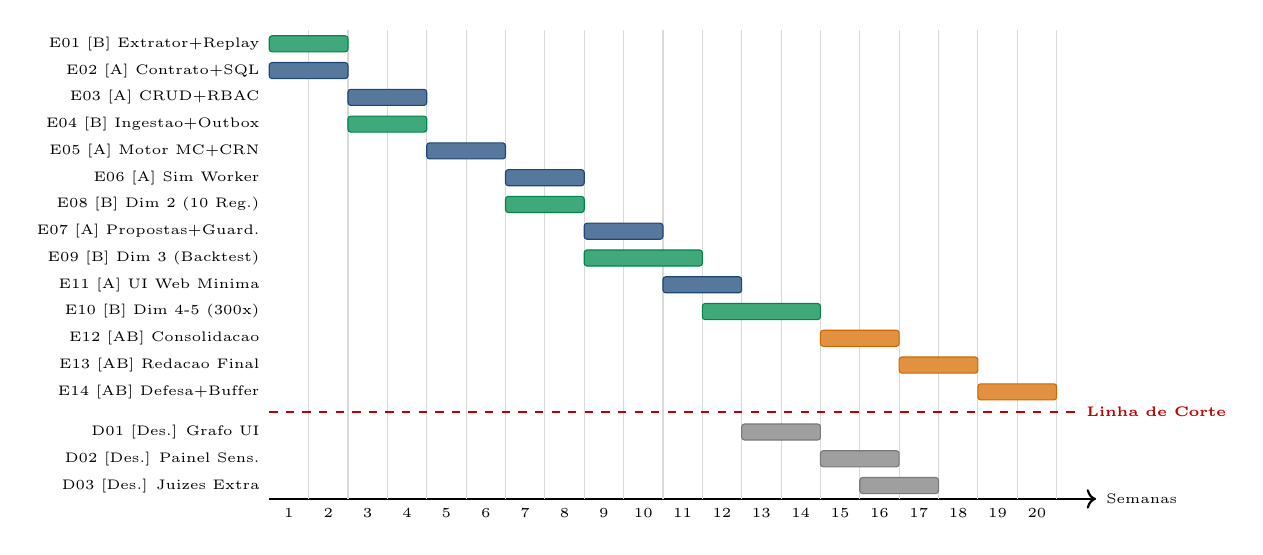
\begin{tikzpicture}[x=0.50cm,y=0.34cm, font=\tiny]
  \draw[->, thick] (0,0) -- (21,0) node[right]{Semanas};
  \foreach \w in {1,2,...,20} {
    \draw[gray!30] (\w,0) -- (\w,17.5);
    \node[below] at (\w-0.5, 0) {\w};
  }
  \foreach \row/\lbl/\s/\e/\col in {
    17/{E01 [B] Extrator+Replay}/0/2/unbgreen,
    16/{E02 [A] Contrato+SQL}/0/2/unbblue,
    15/{E03 [A] CRUD+RBAC}/2/4/unbblue,
    14/{E04 [B] Ingestao+Outbox}/2/4/unbgreen,
    13/{E05 [A] Motor MC+CRN}/4/6/unbblue,
    12/{E06 [A] Sim Worker}/6/8/unbblue,
    11/{E08 [B] Dim 2 (10 Reg.)}/6/8/unbgreen,
    10/{E07 [A] Propostas+Guard.}/8/10/unbblue,
    9/{E09 [B] Dim 3 (Backtest)}/8/11/unbgreen,
    8/{E11 [A] UI Web Minima}/10/12/unbblue,
    7/{E10 [B] Dim 4-5 (300x)}/11/14/unbgreen,
    6/{E12 [AB] Consolidacao}/14/16/orange!85!black,
    5/{E13 [AB] Redacao Final}/16/18/orange!85!black,
    4/{E14 [AB] Defesa+Buffer}/18/20/orange!85!black,
    2.5/{D01 [Des.] Grafo UI}/12/14/gray,
    1.5/{D02 [Des.] Painel Sens.}/14/16/gray,
    0.5/{D03 [Des.] Juizes Extra}/15/17/gray%
  } {
    \node[left, font=\tiny] at (0, \row) {\lbl};
    \fill[\col!75, draw=\col!95!black, rounded corners=1pt] (\s, \row-0.30) rectangle (\e, \row+0.30);
  }
  \draw[dashed, thick, red!75!black] (0, 3.25) -- (20.5, 3.25) node[right, font=\bfseries\tiny]{Linha de Corte};
\end{tikzpicture}%
}

\subsection{Avaliação do Cronograma do TCC2 pelo Motor de Monte Carlo da PoC}\label{sec:sim_tcc2}

Para aplicar o método proposto ao próprio planejamento do trabalho, o DAG dos pacotes essenciais \texttt{E01} a \texttt{E14} (incluindo tanto as dependências lógicas entre trilhas quanto as arestas $FS$ que serializam a execução dentro da Trilha A e dentro da Trilha B) foi instanciado na função \texttt{buildTCC2ScheduleNetwork} (\texttt{Codigo/main.go}) e avaliado pelo teste \texttt{TestTCC2ScheduleMonteCarlo} com $N=10.000$ iterações, semente $S_0=42$ e meta de entrega $T_{\mathrm{meta}} = 20{,}0$ semanas úteis. Foram comparadas duas configurações: (i) \textbf{Base PERT-Beta} (apenas incerteza de três pontos nas 14 tarefas essenciais) e (ii) \textbf{Com Riscos Discretos Ativos}, incorporando três riscos da Tabela~\ref{tab:riscos}: \texttt{R\_DAG} em \texttt{E01} ($p=0{,}30, \Delta=1{,}0$ sem., necessidade de ajuste nas heurísticas de extração do DAG), \texttt{R\_LEAK} em \texttt{E09} ($p=0{,}25, \Delta=1{,}0$ sem., ajustes de agrupamento hierárquico e filtragem causal) e \texttt{R\_LLM} em \texttt{E10} ($p=0{,}30, \Delta=1{,}0$ sem., contenção de cota/latência nos 300 cenários e rotulagem da ablação). A Tabela~\ref{tab:sim_tcc2} apresenta os resultados obtidos.

\begin{table}[htbp]
\caption{Simulação de Monte Carlo do cronograma pré-registrado do TCC2 pelo motor \texttt{poc-engine} ($N=10.000$, semente 42, meta de 20 semanas).}\label{tab:sim_tcc2}
\scriptsize
\begin{tabularx}{\textwidth}{X c c c c c c}
\toprule
\textbf{Configuração do Cronograma TCC2} & \textbf{CPM} & \textbf{Média $\bar{F}$ ($\pm$MCSE)} & \textbf{$P_{50}$ ($\pm$MCSE)} & \textbf{$P_{85}$ ($\pm$MCSE)} & \textbf{$P_{95}$ ($\pm$MCSE)} & \textbf{$P(F\le 20)$}\\
\midrule
1. Base PERT-Beta (sem riscos discretos) & 16,75 & 16,81 ($\pm 0{,}007$) & 16,80 ($\pm 0{,}010$) & 17,51 ($\pm 0{,}013$) & 17,94 ($\pm 0{,}015$) & 100,0\%\\
2. Com Riscos Discretos (\texttt{R\_DAG}, \texttt{R\_LEAK}, \texttt{R\_LLM}) & 16,75 & 17,34 ($\pm 0{,}009$) & 17,29 ($\pm 0{,}011$) & 18,30 ($\pm 0{,}014$) & 18,92 ($\pm 0{,}021$) & 99,6\%\\
\bottomrule
\end{tabularx}
\par\vspace{1mm}{\small Fonte: Saída reprodutível de \texttt{go test -v -run TestTCC2ScheduleMonteCarlo} (\texttt{Docs/resultados\_poc.tex}). Índices de Criticidade com riscos ativos: $\IC(\text{E02})=\IC(\text{E03})=\IC(\text{E05})=99{,}2\%$; ramo experimental $\IC(\text{E08})=\IC(\text{E09})=84{,}9\%$ vs. ramo de serviços $\IC(\text{E06})=\IC(\text{E07})=15{,}1\%$; convergência $\IC(\text{E10})=\IC(\text{E12})=\IC(\text{E13})=\IC(\text{E14})=100{,}0\%$; folga paralela em $\IC(\text{E11})=0{,}0\%$.}
\end{table}

A simulação do cronograma na Tabela~\ref{tab:sim_tcc2} revela três conclusões práticas para a gestão do TCC2:
\begin{enumerate}
  \item \textbf{Condicionalidade à alocação estática em duas trilhas (aproximação não-RCPSP):} como o motor modela restrições de recursos por meio de arestas $FS$ que fixam a ordem de execução dentro da Trilha A (Autor 1) e dentro da Trilha B (Autor 2), os percentis reportados ($P_{85}=18{,}30$ semanas e $P_{95}=18{,}92$ semanas com riscos discretos, frente ao horizonte de 20 semanas) são estritamente \textbf{condicionais a essa atribuição estática}, não constituindo resolução dinâmica do problema de escalonamento com restrição de recursos (RCPSP);
  \item \textbf{Identificação do caminho crítico estocástico do TCC2:} entre os pacotes paralelos intermediários, o ramo experimental da Trilha B (\texttt{E08} $\rightarrow$ \texttt{E09}, com $\IC = 84{,}9\%$ sob riscos ativos) domina o ramo de acoplamento do worker e governança da Trilha A (\texttt{E06} $\rightarrow$ \texttt{E07}, com $\IC = 15{,}1\%$) antes da convergência obrigatória em \texttt{E10} ($\IC = 100{,}0\%$), enquanto a interface web mínima (\texttt{E11}, executada na Trilha A em paralelo a \texttt{E10}) apresenta folga determinística e estocástica ($\IC = 0{,}0\%$);
  \item \textbf{Pré-registro de estimativas e política de corte de escopo:} as estimativas O/M/P da Tabela~\ref{tab:cronograma} encontram-se pré-registradas no código-fonte da PoC (\texttt{buildTCC2ScheduleNetwork}). Caso desvios reais durante o TCC2 desloquem o quantil $P_{85}$ atualizado para além de 20,0 semanas nas rodadas de monitoramento quinzenal, a resposta governada será o \textbf{corte de escopo} — descartando integralmente os pacotes desejáveis \texttt{D01} a \texttt{D03} e reduzindo a interface \texttt{E11} para inspeção tabular estática —, vedando-se o ajuste artificial de estimativas para caber no calendário.
\end{enumerate}

\section{Matriz de Riscos da Pesquisa}

A Tabela~\ref{tab:riscos} sintetiza os riscos técnicos e metodológicos mapeados para o TCC2 e as respectivas estratégias de mitigação e contingência.

\begin{table}[htbp]
\caption{Matriz de riscos da pesquisa e estratégias de mitigação no TCC2.}\label{tab:riscos}
\footnotesize
\begin{tabularx}{\textwidth}{L{3.8cm} c c Y}
\toprule
\textbf{Risco identificado} & \textbf{Impacto} & \textbf{Prob.} & \textbf{Mitigação e plano de contingência}\\
\midrule
Baixa densidade de dependências $FS$ explícitas no GitHub CLI (\texttt{R\_DAG}: $p=0{,}30, \Delta=1{,}0$ sem.) & Alto & Média & Piloto de extração do DAG nas Semanas 1--2 (E01), combinando links explícitos (\texttt{closes/depends on}) com dependências de módulos e mantendo a Dimensão 3 como descritiva complementar à Dimensão 2\\
Viés de construto por abertura tardia de PRs & Alto & Alta & Medição já corrigida no extrator a partir de $\min(\texttt{first\_commit\_at}, \texttt{assigned\_at}, \texttt{pr\_created\_at})$ até o \texttt{merged\_at} com piso de $0{,}25$ d.u.\\
Ajustes de agrupamento hierárquico e filtragem no \textit{backtesting} (\texttt{R\_LEAK}: $p=0{,}25, \Delta=1{,}0$ sem.) & Médio & Baixa & Exigência de $n_{\text{classe}}\ge 15$ com \textit{shrinkage} para o pool global, ajuste no subconjunto limpo e \textit{fallback} de \textit{bootstrap} empírico (E09)\\
Latência/cota de API e rotulagem nas 300 execuções da IA (\texttt{R\_LLM}: $p=0{,}30, \Delta=1{,}0$ sem.) & Alto & Média & Uso combinado de modelo local (\texttt{Llama-3.3-70B}) e API com cache determinístico, extrator pré-fixado e 3 juízes em subamostra de 50 pares (E10)\\
Injeção indireta de \textit{prompt}, XSS ou persuasão do aprovador & Alto & Média & Sub-rede isolada (\texttt{ai-isolated-net}), validação \textit{fail-closed}, CSP estrito, cartão determinístico segregado e alerta simétrico de deriva $\pm 30\%$\\
Adulteração direta da tabela \texttt{audit\_logs} no banco & Médio & Baixa & Revogação de permissões SQL, \textit{trigger} de bloqueio, cadeia SHA-256 e exportação assinada do \texttt{head\_hash} para âncora externa WORM\\
\bottomrule
\end{tabularx}
\fonteautores
\end{table}

\section{Limitações Declaradas}\label{sec:limitacoes}

Por transparência científica, declaram-se oito limitações de escopo deste trabalho:
\begin{enumerate}
  \item \textbf{Capacidade infinita de recursos na rede geral e alocação estática de trilhas:} o cálculo básico de CPM e Monte Carlo assume capacidade irrestrita para tarefas paralelas sem aresta lógica, e a simulação do cronograma do TCC2 serializa pacotes por autor mediante arestas $FS$ fixas (aproximação estática condicional à atribuição, e não resolução dinâmica de RCPSP);
  \item \textbf{Independência condicional na formulação nominal:} o motor básico sorteia as durações Beta de forma independente entre tarefas, capturando acoplamento apenas pela topologia do grafo e por riscos discretos; o impacto de correlações fortes ($\rho=0{,}50$) será caracterizado no Regime R9 da Dimensão 2;
  \item \textbf{Escalonamento linear do trabalho e risco remanescentes:} a redução proporcional por $(1-c_i)$ tanto da duração base quanto do impacto de riscos discretos é uma aproximação linear de primeira ordem que pode subestimar riscos concentrados na integração final;
  \item \textbf{Efeito residual de persuasão e viés de automação humano:} embora a interface segregue visualmente os deltas determinísticos ($\Delta P_{50}, \Delta P_{85}$) do texto interpretativo não verificado da IA e o servidor emita alertas simétricos de deriva ($\pm 30\%$), nenhuma barreira puramente técnica elimina por completo a complacência ou o viés de automação de um aprovador humano;
  \item \textbf{Truncamento residual na cauda extrema da distribuição Beta:} mesmo com a extensão do suporte $[t_o, t_p]$ por casamento dos quantis teóricos de 10\% e 90\% e estimativa modal HSM, a distribuição Beta mantém suporte limitado, podendo subestimar eventos extremos de cauda pesada (avaliados no Regime R8 da Dimensão 2 e pela variante de \textit{bootstrap} no pacote E09);
  \item \textbf{Generalização empírica restrita e tamanho amostral efetivo no \textit{backtesting}:} a avaliação histórica da Dimensão 3 baseia-se em um único repositório de código aberto em Go (\texttt{cli/cli}) com 10 \textit{releases} consecutivas ($n_{\mathrm{ef}}=10$ unidades independentes em 30 cortes correlacionados), possuindo caráter estritamente descritivo;
  \item \textbf{Atuação restrita ao nível de Sombra Digital Governada:} por decisão de segurança contra agência excessiva (OWASP LLM06:2025), o sistema não executa mutações automáticas não supervisionadas no repositório GitHub nem na linha de base oficial;
  \item \textbf{Alcance da Prova de Conceito no TCC1:} a PoC verifica a corretude algorítmica do CPM, a aderência do amostrador PERT-Beta à distribuição teórica especificada, a reprodutibilidade determinística por índice e o desempenho em memória, cabendo ao TCC2 a integração dos serviços e o teste empírico das hipóteses H1a, H1b, H2a e H2b e dos critérios CA1 e CA2.
\end{enumerate}

\section{Considerações Finais do TCC1}

Este trabalho especificou e fundamentou a arquitetura proposta de uma Sombra Digital Governada para apoio à decisão tática em cronogramas de projetos de software, integrando captura de eventos GitHub/CI, Método do Caminho Crítico, Simulação de Monte Carlo (PERT-Beta acoplada a riscos de Bernoulli) e recomendações interpretativas por um agente LLM isolado da rede do banco de dados. A governança foi estruturada sobre três mecanismos determinísticos: filtragem de entrada por \textit{allowlist} sanitizada, classificação binária de saída com negação por padrão (\textit{fail-closed}) aliada a fila de aprovação humana com pré-visualização de impacto e travas simétricas de deriva, e trilha de auditoria encadeada por SHA-256 com ancoragem externa.

A Prova de Conceito implementada em Go (\texttt{poc-engine}) verificou a viabilidade algorítmica, estatística e computacional do núcleo estocástico: as amostras geradas pelo amostrador PERT-Beta aderem à distribuição teórica especificada nos momentos analíticos e no teste de Kolmogorov-Smirnov ($n=10^6$, $D_n < D_{\mathrm{crit},0{,}05} = 0{,}001358$, $H_0$ não rejeitada), o caso degenerado $t_o=t_p$ é tratado sem indefinições numéricas, a execução concorrente com 1, 4 e 16 \textit{workers} produz quantis e média compensada de Kahan idênticos, e 10.000 simulações em uma rede de 200 tarefas e 300 dependências completam-se em mediana de $62{,}3$ ms com 8 \textit{workers} ($259{,}6$ ms em 1 vCPU). Por fim, a extração auditável de dados do repositório GitHub CLI permitiu contrastar empiricamente o tempo de revisão do PR com a duração desde o primeiro \textit{commit}, resultando em um protocolo experimental de cinco dimensões e em um cronograma pré-registrado de 20 semanas para dois autores cuja própria simulação de Monte Carlo indica $P_{50}=17{,}29$ e $P_{85}=18{,}30$ semanas ($P(F \le 20) = 99{,}6\%$ com riscos discretos).

% =====================================================================
\postextual
\bibliographystyle{abntex2-alf}
\bibliography{referencias}

\begin{apendicesenv}
\partapendices

\chapter{Decisões de Implementação e Contratos do MVP (TCC2)}\label{apd:mvp}

Este apêndice consolida as decisões de engenharia de software e de pilha tecnológica para a construção integradora do MVP nos pacotes E02 a E11 do TCC2:
\begin{itemize}
  \item \textbf{Isolamento de contêineres e sub-redes (Docker Compose):} implantação declarativa \cite{merkel2014} com duas redes bridge isoladas (\texttt{core-net} com \texttt{internal: true} para o PostgreSQL 16 e o \textit{Simulation Worker}; \texttt{ai-isolated-net} restrita à comunicação HTTP entre \textit{Core PM Service} e \textit{AI Agent Service});
  \item \textbf{Interface web mínima (React, TypeScript e Vite) e Server-Sent Events (SSE):} SPA construída com Vite \cite{vite2024} consumindo eventos unidirecionais padronizados pelo W3C \cite{w3c2015} para atualização reativa de curvas CDF e da fila de aprovação, protegida por cabeçalho \texttt{Content-Security-Policy: default-src 'self'; script-src 'self'; object-src 'none'} e renderização exclusiva em texto puro (mitigação de \texttt{LLM05:2025});
  \item \textbf{Fila assíncrona transacional:} a tabela \texttt{simulation\_jobs} é consumida pelos processos do \textit{Simulation Worker} via \texttt{SELECT id, payload FROM simulation\_jobs WHERE status = 'PENDING' ORDER BY created\_at FOR UPDATE SKIP LOCKED} no PostgreSQL 16 \cite{postgresql2024}, garantindo semântica \textit{at-least-once} sem necessidade de manter corretores externos;
  \item \textbf{Agrupamento temporal (\textit{Debounce}) e controle de cota da IA:} janela deslizante configurável de 30 s no \textit{Core PM Service} que agrupa rajadas de \textit{webhooks} em uma única transição consolidada de \texttt{state\_version}, disparando o \textit{AI Agent Service} apenas sob gatilho condicional de relevância ($|\Delta P_{85}| \ge 0{,}5$ d.u., $|\Delta\IC_i| \ge 10$ p.p. ou falha operacional) e limite de 6 chamadas/minuto (\texttt{LLM10:2025});
  \item \textbf{Invalidação de cenários obsoletos e idempotência:} toda simulação grava \texttt{base\_state\_version} (recebendo \texttt{is\_stale = true} caso o estado avance antes da decisão humana), com chaves únicas (\texttt{UNIQUE}) sobre \texttt{X-GitHub-Delivery} (\texttt{delivery\_id}) e \texttt{idempotency\_key}.
\end{itemize}

\chapter{Extração Reprodutível do Dataset e Repositório da PoC}\label{apd:extracao}

Para assegurar reprodutibilidade integral dos resultados reportados nas Tabelas~\ref{tab:backtesting}, \ref{tab:resultados}, \ref{tab:ic}, \ref{tab:momentos}, \ref{tab:repro}, \ref{tab:bench} e \ref{tab:sim_tcc2}, os artefatos de código e dados estão estruturados no repositório público do projeto:

\begin{itemize}
  \item \textbf{URL do Repositório Público:} \url{https://github.com/carlinn1/TCC-01} (repositório público com código-fonte da PoC, \textit{scripts} de extração/figuras e instantâneo JSON pseudonimizado preparado para depósito no Zenodo sob licença aberta);
  \item \textbf{Estrutura de diretórios do repositório:}
  \begin{itemize}
    \item \texttt{Codigo/}: pacote Go 1.22 do motor \texttt{poc-engine} (\texttt{go.mod}, \texttt{model.go}, \texttt{random.go}, \texttt{cpm.go}, \texttt{simulator.go}, \texttt{main.go}, \texttt{engine\_test.go}, \texttt{validation\_test.go}), que exporta automaticamente \texttt{poc\_results.json} e as macros LaTeX em \texttt{Docs/resultados\_poc.tex};
    \item \texttt{Codigo/extract\_dataset.py}: \textit{script} em Python 3.11+ que consulta a API REST e o histórico Git do repositório \texttt{cli/cli}, filtra contas \texttt{Bot}, separa fechamentos \texttt{completed} de \texttt{not\_planned} e PRs fechados sem \textit{merge}, calcula tanto o tempo de revisão do PR quanto a duração de engenharia desde o primeiro \textit{commit} (com piso de $0{,}25$ d.u.), remove qualquer identificador pessoal (PII/logins) e oferece verificação local offline (\texttt{--verify-local});
    \item \texttt{Codigo/dataset\_backtesting.json}: instantâneo auditável e pseudonimizado das três janelas do \texttt{cli/cli};
    \item \texttt{Codigo/generate\_figures.py} e \texttt{Docs/figuras/}: gerador reprodutível das 8 imagens PNG RGB opacas em 200 DPI referenciadas em \texttt{Docs/Main.tex};
  \end{itemize}
  \item \textbf{Comandos exatos de reprodução:}
  \begin{enumerate}
    \item Geração e sincronização das 8 figuras PNG (200 DPI RGB opaco):
    \texttt{cd Codigo \&\& python3 generate\_figures.py}
    \item Verificação funcional, analítica, teste KS, caso degenerado, reprodutibilidade entre \textit{workers}, simulação do cronograma do TCC2 e exportação de \texttt{Docs/resultados\_poc.tex}:
    \texttt{cd Codigo \&\& go test -count=1 -v ./... \&\& go run .}
    \item Execução das 5 repetições dos \textit{benchmarks} de desempenho e memória:
    \texttt{cd Codigo \&\& go test -bench=Benchmark -benchmem -count=5}
    \item Verificação de integridade e ausência de PII do dataset local (ou reextração via Git/API):
    \texttt{python3 Codigo/extract\_dataset.py --verify-local --out Codigo/dataset\_backtesting.json}
  \end{enumerate}
\end{itemize}

\end{apendicesenv}

\end{document}